\documentclass[12pt,a4paper,final,twoside]{book}
\usepackage[utf8]{inputenc}
\usepackage[spanish]{babel}
\usepackage{url}
\usepackage{graphicx}
\usepackage{hyperref}
\usepackage{amsmath,amssymb,amsthm,amscd}
\usepackage{setspace}
\onehalfspacing
\usepackage{multirow}

\usepackage{eurosym}

\usepackage{caption}
\usepackage{subcaption}
\usepackage{framed}

%plots
\usepackage{tikz}
\usepackage{pgfplots}
\usepgfplotslibrary{statistics}
\usetikzlibrary{patterns}

\usepackage[ampersand]{easylist} 
%\usepackage{epstopdf}
\usepackage{array}
\usepackage{tabulary}

\usepackage{float}

\usepackage[left=2.5cm,right=2.5cm,top=2.5cm,bottom=2.5cm]{geometry}

\usepackage{appendix}
\renewcommand{\appendixname}{Anexos}
\renewcommand{\appendixtocname}{Anexos}
\renewcommand{\appendixpagename}{Anexos}
\makeindex

\usepackage{wrapfig}

\usepackage{pgfgantt}

\usepackage{fancyhdr}
\pagestyle{fancy}
\fancyhead{}
\fancyhead[RO,LE]{\thepage}
\fancyhead[RE,LO]{Integración de la plataforma AIBO con ROS }
\fancyfoot{}
\fancyfoot[RO,LE]{
\includegraphics[scale=0.18]{images/etseib.pdf}}
\headheight = 15pt 
\textheight = 690pt 
\footskip = 2 cm

\usepackage{anysize} 
\marginsize{3cm}{2cm}{2cm}{2cm} 

\usepackage[numbers]{natbib}
\usepackage{listings}
\usepackage{color}

\definecolor{mygreen}{rgb}{0,0.6,0}
\definecolor{mygray}{rgb}{0.5,0.5,0.5}
\definecolor{mymauve}{rgb}{0.58,0,0.82}
\definecolor{barblue}{RGB}{0,119,255}
\lstset{ %
  backgroundcolor=\color{white},   % choose the background color; you must add \usepackage{color} or \usepackage{xcolor}
  basicstyle=\footnotesize,        % the size of the fonts that are used for the code
  breakatwhitespace=false,         % sets if automatic breaks should only happen at whitespace
  breaklines=true,                 % sets automatic line breaking
  captionpos=b,                    % sets the caption-position to bottom
  commentstyle=\color{mygreen},    % comment style
  deletekeywords={...},            % if you want to delete keywords from the given language
  escapeinside={\%*}{*)},          % if you want to add LaTeX within your code
  extendedchars=true,              % lets you use non-ASCII characters; for 8-bits encodings only, does not work with UTF-8
  frame=single,                    % adds a frame around the code
  keepspaces=true,                 % keeps spaces in text, useful for keeping indentation of code (possibly needs columns=flexible)
  keywordstyle=\color{black},       % keyword style
  language=Octave,                 % the language of the code
  morekeywords={*,...},            % if you want to add more keywords to the set
  numbers=left,                    % where to put the line-numbers; possible values are (none, left, right)
  numbersep=5pt,                   % how far the line-numbers are from the code
  numberstyle=\tiny\color{mygray}, % the style that is used for the line-numbers
  rulecolor=\color{black},         % if not set, the frame-color may be changed on line-breaks within not-black text (e.g. comments (green here))
  showspaces=false,                % show spaces everywhere adding particular underscores; it overrides 'showstringspaces'
  showstringspaces=false,          % underline spaces within strings only
  showtabs=false,                  % show tabs within strings adding particular underscores
  stepnumber=2,                    % the step between two line-numbers. If it's 1, each line will be numbered
  stringstyle=\color{black},     % string literal style
  tabsize=2,                       % sets default tabsize to 2 spaces
  title=\lstname                   % show the filename of files included with \lstinputlisting; also try caption instead of title
}
\bibliographystyle{plainnat} 
\title{Implementación de }
\author{Diego Muñoz Galan}

\begin{document}

\maketitle
\thispagestyle{empty}

\newpage
\paragraph{}
\thispagestyle{empty}
\cleardoublepage

\setcounter{page}{1}
\begin{center}
\section*{Resumen}
\end{center}

\addcontentsline{toc}{section}{Resumen}
El proyecto persigue el objetivo de implementar un driver para integrar la plataforma robótica AIBO con el marco de trabajo ROS. A lo largo de esta memoria se narra el procedimiento seguido para llegar a un resultado que cumpla con los requisitos. 
Se puede dividir el trabajo realizado y documentado en ésta memoria en tres partes.

Consta de una primera parte de documentación e investigación de la plataforma objeto en la que se describe tanto el hardware como los posibles softwares con los que trabajar.

Sigue una segunda parte en la que se comparan varios métodos de programación con los que se podría implementar el modulo de ROS deseado. En ésta se incluye un primer análisis cualitativo en el que se contemplan gran parte de las posibilidades de programación y un segundo análisis más exhaustivo de los métodos que han pasado la primera selección para finalmente decidir el método a usar.

Para concluir se explica como se han implementado los módulos que facilitan la integración con ROS. Por un lado el modulo de control al que se le han aplicado unos criterios de valoración y se ha puesto a prueba y por otro el modulo que facilita la integración de un modelo de visualización 3D.




\newpage
\thispagestyle{empty}
\cleardoublepage

\tableofcontents
\newpage
\listoffigures
\newpage
\listoftables
\newpage


\section{Prefacio}
\subsection{Motivación}
Hace ya ocho años que la empresa SONY dejó de producir la mascota robótica por excelencia, el perro robot AIBO \cite{aibo}. Des de su desaparición del mercado, en 2006, éste ha caído en una espiral de desuso hasta el punto que hoy en día se pueden encontrar gran cantidad de ellos guardados en armarios de todo el mundo.

Este proyecto partió de la idea de volver a aprovechar los AIBO para realizar tareas de cooperación y sincronización partiendo de un nivel de programación elevado. Debido a la incomodidad que proporcionaban los actuales lenguajes de programación para dicha plataforma, dado que ya no están siendo mantenidos y sus curvas de aprendizaje son realmente duras,   se planteó la posibilidad de programar al AIBO mediante ROS\cite{ros}.
Siendo ROS uno de los marcos de trabajo para la robótica que actualmente está teniendo más acogida, su uso sobre AIBO haría posible que volvieran a ser una plataforma a tener en cuenta para la investigación en estos momentos en que la universidad no cuenta con demasiados fondos. Por el otro lado la implementación de un driver para AIBO facilitará enormemente la programación, dando la posibilidad de usar el gran abanico de paquetes y herramientas existentes para ROS.

Por estos motivos participar en la integración del AIBO con ROS es un proyecto que dado su posible utilidad en el futuro lo hace irresistible.

Además el propio aprendizaje intrínseco del proyecto como es la oportunidad de conocer y entender ROS implementando ciertos paquetes resulta algo realmente interesante y útil para cualquier estudiante apasionado por la robótica.


\subsection{Requerimientos previos}
Para la realización de este proyecto es necesario un cierto bagaje y experiencia en programación, concretamente en los lenguajes C++ y python orientados a objetos, además de un conocimiento básico del funcionamiento de ROS y su estructura.
Son necesarios también conocimientos de estadística y el uso de software de apoyo para la realización de algunos testes estadísticos.
Por ultimo para la realización del proyecto se ha hecho uso de la herramienta \LaTeX. 
\newpage
\clearpage

\section{Introducción}
En este apartado se definirá tanto el punto de partida del proyecto, el punto final al que se pretende llegar y el camino que se pretende realizar. 
 
\subsection{Estado del arte}\label{estatdelart}
Se pretende dar una visión general del estado actual de la robótica y el compromiso entre software y hardware que ésta conlleva para seguidamente ir concretando y acotando sobre este gran universo hacia el punto que ocupa éste proyecto. 

\subsubsection{Robótica}

Desde la primera definición de robot o de la idea que exporto Isaac Asimov ha pasado más de medio siglo y aún así se puede decir que la robótica se encuentra dando sus primeros pasos. Si bien no es sencillo ubicar el origen de esta ciencia se puede afirmar con total seguridad que esta rama hizo grandes avances a raíz de la revolución industrial de mano de otras especialidades como la electrónica, la informática o la inteligencia artificial.

En un primer momento los robots fueron máquinas automatizadas o teleoperadas con el fin de realizar tareas dentro de la industria que tuvieran un cierto riesgo, requiriesen de alta precisión o una eficiencia tal que la mano de obra humana no pudiera ofrecer. En este contexto actualmente se encuentran gran variedad de brazos manipuladores en la mayoría de las fabricas que a la vez que aumentan su grado automatización, la eficiencia y rentabilidad económica lo hacen con el\cite{libroblanco}. Un ejemplo de este tipo de robots son los de KUKA\footnote{\url{http://www.kuka-robotics.com/en/}} mostrado en la Figura \ref{fig:kuka}.
 
\begin{figure}[h!]
	\centering
    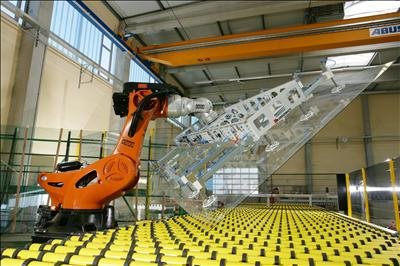
\includegraphics[scale=3]	{images/kuka.jpg}
	 \caption{Robot manipulador de KUKA.}
  \label{fig:kuka}
\end{figure}

Otros sectores, aparte de la industria, han impulsado la robótica dando pie a otro tipo de robots, los robots móviles. Éste es el caso de la exploración espacial que dio sus primeros pasos con el automóvil teleoperado lunokjod\footnote{\url{http://en.wikipedia.org/wiki/Lunokhod_1}} y actualmente tiene su máximo exponente con el robot Curiosityenviado a Marte en la última misión de la NASA\footnote{\url{http://www.nasa.gov/mission_pages/msl/}}. Las plataformas anteriormente descritas tienen la sencillez de moverse sobre ruedas, a diferencia de otro tipo de robots móviles que usan varias extremidades, bípedos, cuadrúpedos, hexápedos y otros con gran cantidad de ellas. Si bien el uso de extremidades dificulta el control dinámico, la estabilidad y los algoritmos de  navegación, ofrecen la posibilidad de andar por gran variedad de terrenos y producen una mayor aceptación social debido a su morfología familiar para el hombre . Un ejemplo es el robot cuadrúpedo de DARPA\footnote{\url{http://www.darpa.mil}} y Boston Dynamics \footnote{\url{http://www.bostondynamics.com/}} Wildcat mostrado a en la Figura \ref{fig:wildcat}.

\begin{figure}[h!]
	\centering
    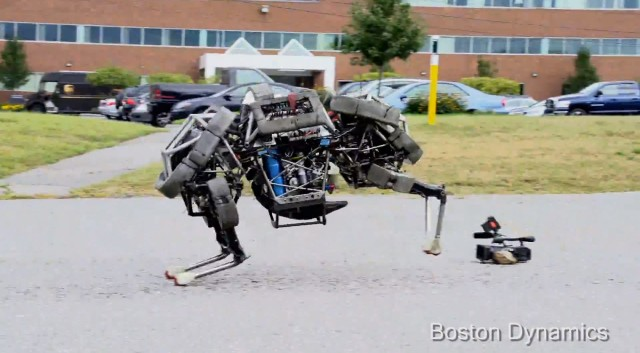
\includegraphics[scale=0.6]	{images/Wildcat.jpg}
	 \caption{Robot cuadrúpedo WildCat.}
  \label{fig:wildcat}
\end{figure}

\subsubsection{Robótica en la educación}

Las plataformas anteriormente descritas forman parte de proyectos millonarios que no forman parte de el grueso de la investigación con robótica.
Son las plataformas como la usada en este proyecto las que han permitido tanto a universidades como a un público mucho más general investigar y han dado la oportunidad de crear una gran variedad de aplicaciones.

Algunos de los robots que han acercado las herramientas necesarias a un mayor número de usuarios son los siguientes: 

\begin{itemize}
\item WIFIBOT: Se trata de una serie de robots movidos por cuatro ruedas, sensores de distancia , camera y punto de acceso WiFi. Permite ser controlado por varios sistemas operativos y lenguajes\footnote{\url{http://www.wifibot.com/}}.
\item Lego NXT: Es un producto modular que permite una infinidad de combinaciones construcitvas partiendo siempre de un módulo de procesador. Tiene su própio marco de trabajo\footnote{\url{http://www.lego.com/en-us/mindstorms/?domainredir=mindstorms.lego.com}}.
\item NAO: Es un robot humanoide de dimensiones reducidas y con prestaciones de alta gama comercializado por Aldebaran Robotics \footnote{\url{http://www.aldebaran.com/en}}.
\item ARDrone: Se trata de un vehículo no tripulado con cuatro hélices, o quadcoptero,  que se respalda tanto la navegación autónoma como el radiocontrol.
\end{itemize}

Habiendo hablado un poco del hardware se pasa a comentar los sistemas más usados para crear la inteligencia artificial.

La gran mayoría de robots, dado que son comercializados por empresas, proporcionan un marco de trabajo propio e incluso su propio lenguaje algorítmico de alto nivel. Facilitando el acceso de forma sencilla a actuadores, sensores y sistemas de comunicación, permitiendo a un amplio público la iniciación en la robótica.
Por otra parte existen ciertos softwares libres que se están estableciendo como una alternativa a los propios de cada plataforma.
Ésto facilita enormemente del trabajo del programador puesto que no tiene que invertir tiempo en el aprendizaje propio de cada software. 
Cabe destacar dos de ellos:

\begin{itemize}
\item URBI\cite{urbiref}: Del cual se pude encontrar información en la Sección \ref{urbi}.
\item ROS: Es el marco de trabajo más extendido actualmente y abasta una gran cantidad de plataformas. En la Sección \ref{ros} se puede encontrar más información.
\end{itemize} 

Por lo que respeta a la implementación de drivers para pasar de un lenguaje propio a ROS Existen varios ejemplos que se pueden encontrar actualmente en la web de ROS este es el caso de ARDrone o Bioloid. 

\subsubsection{AIBO}

Con la plataforma de estudio AIBO Sección \ref{secaibo} se han realizado diversos proyectos de índoles muy diferentes dada su versatilidad. Sobretodo se han llevado a cabo proyectos relacionados con visión \cite{xavi} o comportamientos e inteligencia artificial \cite{riki}.
Un punto esencial en el desarrollo del AIBO fue que durante el período comprendido entre 1999 y 2008 fue la plataforma elegida para realizar la competición RoboCup Estandard Plataform League, posteriormente sustituido por la plataforma NAO. La RoboCup es una competición internacional destinada a promover la robótica y donde se realizan pruebas como la comentada anteriormente que forma parte de la sección de fútbol con robots autónomos. La prueba de simulacros de rescate fue otra donde el AIBO tubo una gran acogida y fue muy usado \cite{robocup}.
La RoboCup fue fuente de inspiración para muchos investigaciones que se pueden clasificar en tres grupos según su finalidad:
\begin{itemize}
\item Visión i reconocimiento de marcas para la posterior ubicación dentro del campo \cite{morales}.
\item Comunicaciones y control sobre los movimientos \cite{jesus}.
\item Definición de roles dentro del campo \cite{metod}.
\end{itemize}

Actualmente el AIBO no se usa como se hacia antes, en parte porque ya no es la plataforma estándar de la RoboCup y en parte porque des de que en 2006 SONY dejo de producirlo su lenguaje base OPEN-R\cite{OPEN-R PG} dejó de ser mantenido.
A medida que ha caído en desuso los softwares que los soportaban ha dejado hacerlo, incluso aquellos que nacieron especialmente para el AIBO. Es el caso de URBI que des de la version 1.5 de su librería, liburbi, no es compatible.
Además la recerca de éste proyecto se ha visto dificultada por la desaparición de la red de gran parte de la documentación de estos lenguajes.

Ha habido otros intentos de recuperación de la plataforma AIBO es el caso de de un proyecto que trataba de hacer compatible la version 2.3 de liburbi para AIBO \cite{kecsap}.
Otro proyecto del que solo se ha conseguido encontrar un articulo que lo mencione y nada de documentación  trataba de realizar la integración mediante EusLisp de a ROS varias plataformas, entre ellas AIBO \cite{euslisp}.


\subsection{Objetivos}
EL objetivo de este proyecto es recuperar al AIBO como plataforma educativa aportándole una capa superior de programación que permita la integración de la plataforma con ROS.
Con este fin  se compararan diversos caminos con tal conseguir el mejor resultado.

Como objetivos concretos se marcan:
\begin{itemize}
\item Buscar la mejor opción de comunicación, entendiendo como mejor un equilibrio entre sencillez y calidad de la comunicación. Ésto conllevará por un lado  un análisis cualitativo de los posibles métodos y un análisis mas exhaustivo de los posibles caminos que hayan pasado la primera selección.

\item La creación de un paquete de ROS que permita extraer todos los valores de los sensores y articulaciones y a su vez permita controlar al AIBO de forma remota.

\item La creación de los paquetes necesarios para demostrar el buen funcionamiento del paquete anteriormente mencionado.

\item La creación de un paquete que incluya un modelo del AIBO que pueda ser integrado dentro de los simuladores y visores del marco de trabajo ROS. 
\end{itemize}

\subsection{Alcance}
El proyecto incluirá:
\begin{itemize}
\item Creación de un paquete de ROS que permita extraer los valores de los sensores y articulaciones así como actuar sobre las últimas y poder controlar el AIBO.
\item Implementación de las pruebas necesarias para fundamentar el resultado de cualquier comparación.
\item Creación de un modelo 3D del AIBO y su descripción en formato URDF (Unified Robots Description Format).
\item Implementación del driver que permita interaccionar el modelo visualizado con rviz y el AIBO real.
\end{itemize} 

No incluirá:
\begin{itemize}
\item La adquisición de los datos obtenidos por la camera o los micrófonos del AIBO.
\item El renderizado del modelo.
\item La dinámica del modelo.
\item La definición de los sensores para el modelo.
\item La descripción del modelo adaptada completamente para el simulador Gazebo\footnote{Es el simulador de licencia libre mas usado en el marco de trabajo de ROS.}
\item La creación de un mapa físico para el uso del modelo.
\end{itemize}


\subsection{Planificación}
El proyecto se llevará a cabo en 17 semanas  distribuyendo las tareas programadas como muestra el diagrama de Gantt de la Figura \ref{fig:diagramagantt}.
\begin{figure}[H]
\begin{center}
%\noindent\resizebox{\textwidth}{21cm}{
\begin{tikzpicture}[x=.5cm, y=0.01cm]

\begin{ganttchart}[
vgrid={*6{draw=none}, dotted},
hgrid,
y unit chart=0.5cm,
bar/.append style={fill=barblue, rounded corners=3pt},
x unit=0.7mm,
bar height=0.35,
]{0}{125}
\gantttitle{2014}{126} \\
\gantttitle{Febrero}{19}
\gantttitle{Marzo}{31}
\gantttitle{Abril}{30}
\gantttitle{Mayo}{31}
\gantttitle{Junio}{15} \\
\gantttitle{semanas}{126}\\
\gantttitlelist{1,...,18}{7}\\
\ganttgroup{Estudio preliminar}{0}{27} \\
\ganttbar{Estudio de la plataforma}{0}{13} \\
\ganttbar{Estudio de los marcos de trabajo}{6}{27} \\

\ganttgroup{Comparación de alternativas}{27}{48} \\
\ganttbar{Diseño de experimentos}{27}{41} \\
\ganttbar{Adquisición de datos}{34}{48} \\
\ganttbar{Análisis de los resultados}{41}{48} \\

\ganttgroup{módulo aibo{\_}server}{48}{97} \\

\ganttbar{Diseño}{48}{62} \\
\ganttbar{Programación}{55}{90} \\
\ganttbar{Depuración}{62}{90} \\
\ganttbar{Programación de tests}{69}{83} \\
\ganttbar{Pruebas y tests}{76}{97} \\

\ganttgroup{módulo aibo{\_}description}{97}{118} \\
\ganttbar{Programación del XML}{97}{111} \\
\ganttbar{Modelado 3D }{104}{111} \\
\ganttbar{Programación del driver}{111}{118} \\

\end{ganttchart}
\end{tikzpicture}
%}

\end{center}
\caption{Diagrama de Gantt}
\label{fig:diagramagantt}
\end{figure}



\newpage
\clearpage

\section{AIBO ERS-7}\label{secaibo}
En 1999 SONY lanzo al mercado la mascota robótica AIBO (Artificial Intelligence roBOt, amigo en japonés). AIBO es un robot conforma de perro 
que fue ideado para interaccionar con su dueño como una mascota real, es capaz de percibir estímulos del exterior mediante una serie de sensores. Lleva incorporado de serie un software llamad AIBO MIND dentro de una tarjeta de memoria que le permite comportarse como un perro real, reconocer a su dueño, reconocer objetos, jugar con una pelota y aprender, entre muchas otras cosas.


\subsection{Hardware}
Sony ha desarrollado varios modelos y versiones del AIBO como del software AIBO MIND, mejorando tanto actuadores y sensores como la inteligencia.

Entre los diferentes modelos existentes se trabajará con el modelo ERS-7, que se caracteriza por tener una camera de mayor resolución y un procesador más potente.

\begin{figure}[h!]
	\centering
    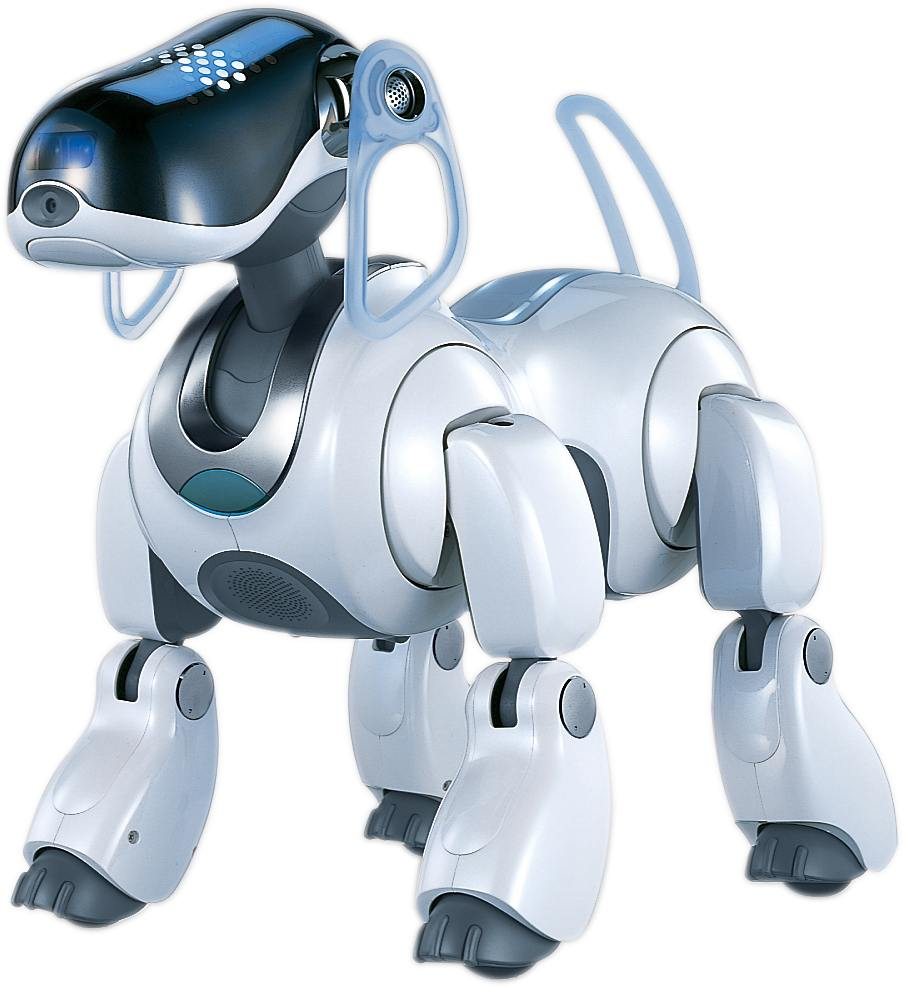
\includegraphics[scale=0.1]	{images/ers7lrg}
	 \caption{AIBO ERS-7.}
  \label{fig:ers7}
\end{figure}	

El AIBO ERS-7 tiene las siguientes características: 

\begin{itemize}
\item Audio:
\begin{itemize}
\item Entrada de audio: Micrófono estéreo.
\item Salida de audio: Altavoces de 20.8 mm i 500 mW.
\end{itemize}
\item Sensores integrados:
\begin{itemize}
\item Sensores de presión:
\begin{itemize}
\item 1 sobre la cabeza.
\item 3 en la espalda.
\end{itemize}
\item 1 sensor de contacto en cada pata. 
\item 1 sensor booleano bajo la boca.
\item Acelerometros en x,y i z.
\item 2 sensores de proximidad de infrarrojos situados en el morro y en el pecho.
\item Sensor de vibración.
\end{itemize}
\item Grados de libertad: Están controlados con motores de continua seguido de una reductora y un encoder absoluto.
\begin{itemize}
\item 3 grados de libertad a cada una de les 4 potes.
\item 3 grados de libertad al cuello..
\item 1 grado de libertad a cada oreja.
\item 1 grado de libertad a la boca.
\item 2 grados de libertad a la cola. 
\end{itemize}
\item Entrada de imagen.
\begin{itemize}
\item Sensor de imagen CMOS de 350000 pixels.
\item Ángulos: 56.9º horizontal i 45.2º vertical.
\item Resoluciones: 208x160, 104x80, 52x40.
\item 30 frames por segundo.
\end{itemize}
\item Dimensiones:
\begin{itemize}
\item Altura: 278 mm.
\item Largo: 319 mm.
\item Ancho: 180 mm.
\item Peso con batería: 1.65 Kg. 
\end{itemize}
\item CPU:
\begin{itemize}
\item Procesador: MIPS R7000 @ 576 MHz.
\item RAM: 64 MB.
\item Memoria flash: 4 MB.
\end{itemize}
\end{itemize}
\begin{itemize}
\item Conectividad:
\begin{itemize}
\item LAN inalámbrico IEEE 802.11b.
\item Xifrat: WEP.
\end{itemize}
\end{itemize}

\subsection{El software}
APERIOS es el sistema operativo en tiempo real que usan los AIBO. Está destinado y diseñado para poder trabajar con grandes flujos de datos de audio e imagen simultaneamente en tiempo real.
En un principio AIBO iba a ser comercializado con una finalidad puramente lúdica, pero debido a su atractivo diseño y su robustez atrajo la atención de programadores que vieron el potencial para convertirse en una herramienta de investigación y aprendizaje. Ésto llevo a SONY a desarrollar un software de desarrollo llamado OPEN-R SDK y que usaba un lenguaje propio, OPEN-R. A raíz de este modulo salieron otros lenguajes e interfaces que trabajaban en una capa superior, sobre OPEN-R y APERIOS, como son \textit{URBI}\footnote{\url{www.urbiforge.org}} o \textit{Tekkotsu}\footnote{\url{tekkotsu.org}}.

\subsubsection{OPEN-R}
OPEN-R es un API en C++ que corre sobre el sistema operativo APERIOS \ref{fig:openrarch}. OPEN-R diferencia entre dos niveles, la capa de sistema por donde se accede al hardware del robot y la capa de aplicación que se trata de los programas hechos por el usuario.

\begin{figure}[h!]
	\centering
    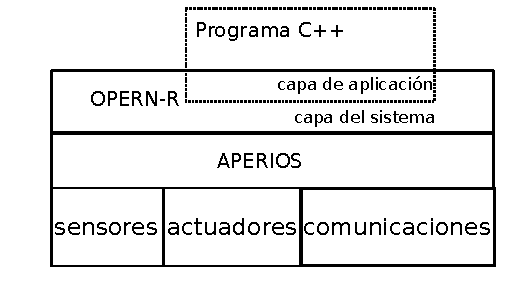
\includegraphics[scale=1]{images/openrarch.pdf}
	 \caption{Arquitectura de AIBO con OPEN-R}
  \label{fig:openrarch}
\end{figure}

Al tratarse de un lenguaje de bajo nivel su estructura es inherente al sistema operativo que se basa en objetos que interaccionan entre si mediante mensajes o meta-objetos. El concepro de objeto es parecido al utilizado en los sistemas \textit{UNIX}\footnote{\url{www.unix.org}} y \textit{Windows}\footnote{\url{http://windows.microsoft.com/en-us/windows/home}}, con la diferencia de que son monohilo y que la comunicación se realiza mediante mensajes que y incluyen datos y un identificador el método en el que se ejecutará en el objeto destino.
Esto implica que cada objetos tiene varios puntos de entrada   y salida que son los métodos:  DoInit(), DoStart(), DoStop(), DoDestroy(). En el paso de mensajes uno se de los objetos se define como sujeto (el que envía) y el otro como observador (el que recibe) que inicia su ejecución después de que el mensaje haga saltar el evento del método correspondiente.

\begin{table}[h]
\begin{center}
\begin{tabulary}{\textwidth}{|C|C|}
\hline
\multirow{1}{*}{\textbf{SUJETO}}
& \textbf{OBSERVADOR} \\ \hline
\multirow{1}{*}{envío de datos}
& \\ \hline
\multirow{1}{*}{notificación del evento}
&  \\ \hline
\multirow{1}{*}{}
& recepción de datos \\ \hline
\multirow{1}{*}{}
& evento preparado \\ \hline
\end{tabulary}
\end{center}
\caption{Estructura del paso de mensajes en OPEN-R\label{msgOR}}
\end{table}
	
\begin{figure}[h!]
	\centering
    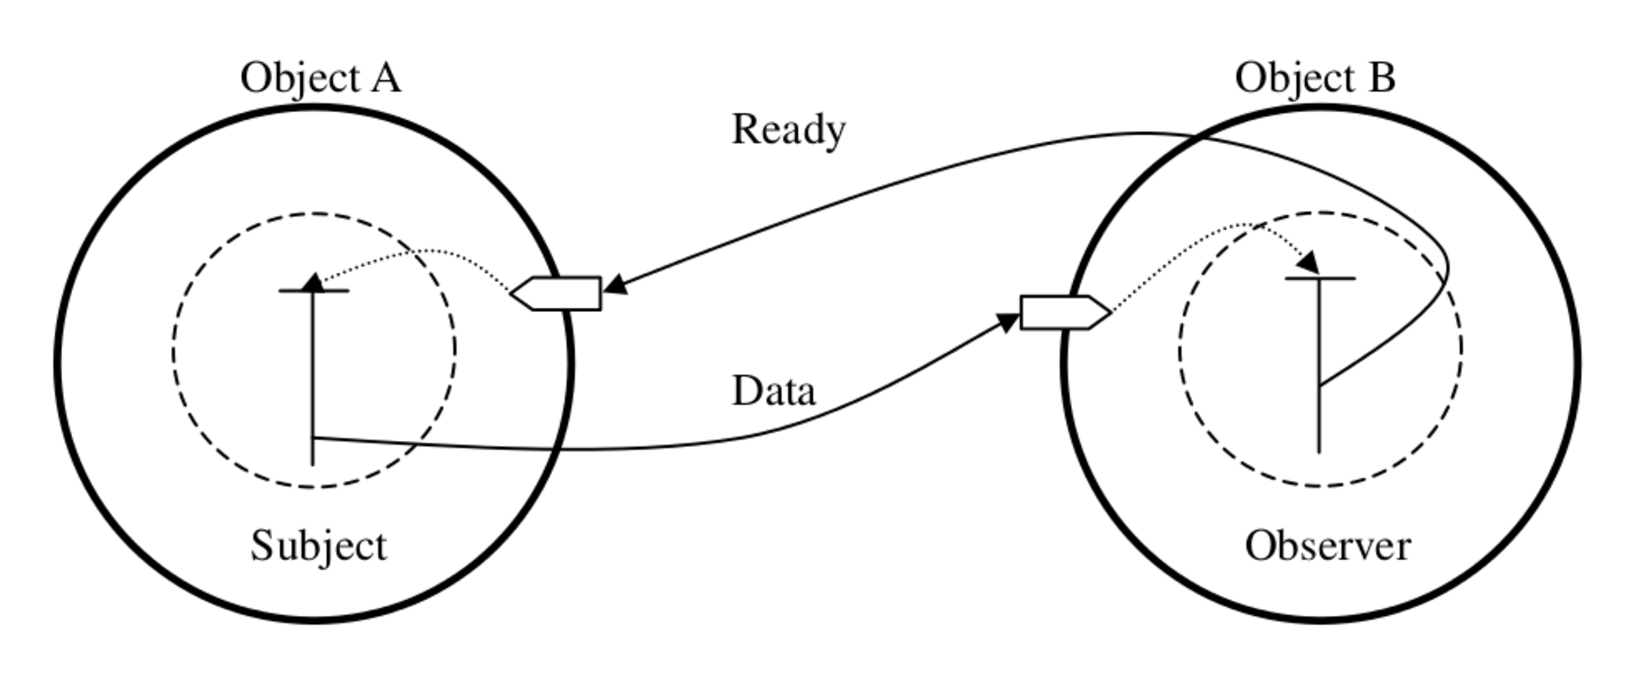
\includegraphics[scale=0.5]{images/ObjectCom.pdf}
	 \caption{Comunicación entre objetos.}
  \label{fig:objectcom}
\end{figure}

Una de las mayores complicaciones que acarrea trabajar con OPEN-R es que usa una gran variedad de archivos que deben ser modificados para poder configurar el programa de aplicación que se realice. Por ello es importante conocer bien los archivos con los que trabaja, los más importantes están listados a continuación: 
:
\begin{itemize}
\item Archivos .h i .cc: Son los archivos de programación de C++.
\item STUB.config: Son archivos de configuración donde se define como un objeto se comunica con los demás.
\item Archivos .ocf: Definen el comportamiento en cuanto a tiempos de ejecución, memória y prioridad de ejecución.
\item Makefile: Archivo para la configuración global de la compilación.
\item OBJECT.cfg: Listado de objetos que se ejecutarán.
\item CONECT.cfg: Se determinan las conexiones entre objetos que se ejecutarán.
\item WLANCONFIG.txt\footnote{Éste ultimo archivo es necesario configurarlo para cualquier método de programación, URBI, Tekkotsu o OPEN-R. Ver APENDIX}: Donde se definen las características de la conexión inalámbrica del AIBO.
\end{itemize}

\subsubsection{Tekkotsu}
Tekkotsu es un software de desarrollo para robots móviles. Orginalmente fue creado para AIBO, pero actualmente permite programar otros plataformas com el Chiara\footnote{\url{http://chiara-robot.org}}, iRobot Create\footnote{\url{http://chiara-robot.org/Create/}}, HandEye\footnote{\url{http://chiara-robot.org/HandEye/}} o Lynxmotion Arms\footnote{\url{http://www.lynxmotion.com/}}.


Mantiene la arquitectura semejante a OPEN-R, basada en objetos y paso de eventos y mantiene la herencia de C++. Proporciona una capa de mayor nivel que OPEN-R pero permite llamar a OPEN-R para acceder de forma rápida a sensores, actuadores y sistemas de comunicación, lo que significa que la capacidad de control sobre el robot se encuentre limitada por el propio hardware y no por el Tekkotsu. Por otro lado permite al usuario trabajar en alto nivel con herramientas de procesamiento visual básico, interfaces de monitorización, modelos de cinemática inversa y soporte para la administración de redes inalámbricas.
 
\begin{figure}[h!]
	\centering
    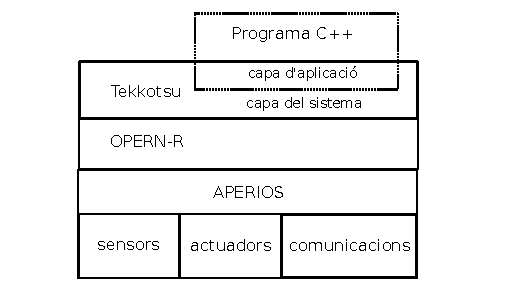
\includegraphics[scale=1.2]{images/tekk.pdf}
	 \caption{Arquitectura del AIBO con Tekkotsu.}
  \label{fig:tekk}
\end{figure}

Además Tekkotsu proporciona una interfaz de usuario, ControllerGUI, que permite acceder al AIBO remotamente y ejecutar los comportamientos que estén programados en la targeta de memoria. Estas funciones se pueden realizar mediante la interfaz gráfica basada en Java como por una conexión telnet\footnote{\url{http://es.wikipedia.org/wiki/Telnet}} al puerto 10020 \cite{TekkQuickRef}.

Tekkots se organiza como un conjunto de comportamientos o \textit{behaviors} y clases llamadas MotionComand. Sus funciones se ejecutan en dos procesos, el \textit{Main} y el \textit{Motion}. El primero se encarga de la percepción i toma de decisiones y el segundo hace referencia al control en tiempo real de los actuadores. Existe un tercer proceso que se encarga de la salida de audio \cite{tekkTut}. 

Los comportamientos, como se llama a todo programa de realizado en Tekkotsu, igual que sus análogos en OPEN-R, tienen una estructura basada en unos métodos que hay que respetar: doStart() y doStop(). Éstos simplifican los cuatro métodos de OPEN-R, pero permiten mantener la estructura y hacen más sencilla y rapida la comunicación.
  
 
\begin{figure}[h!]
	\centering
    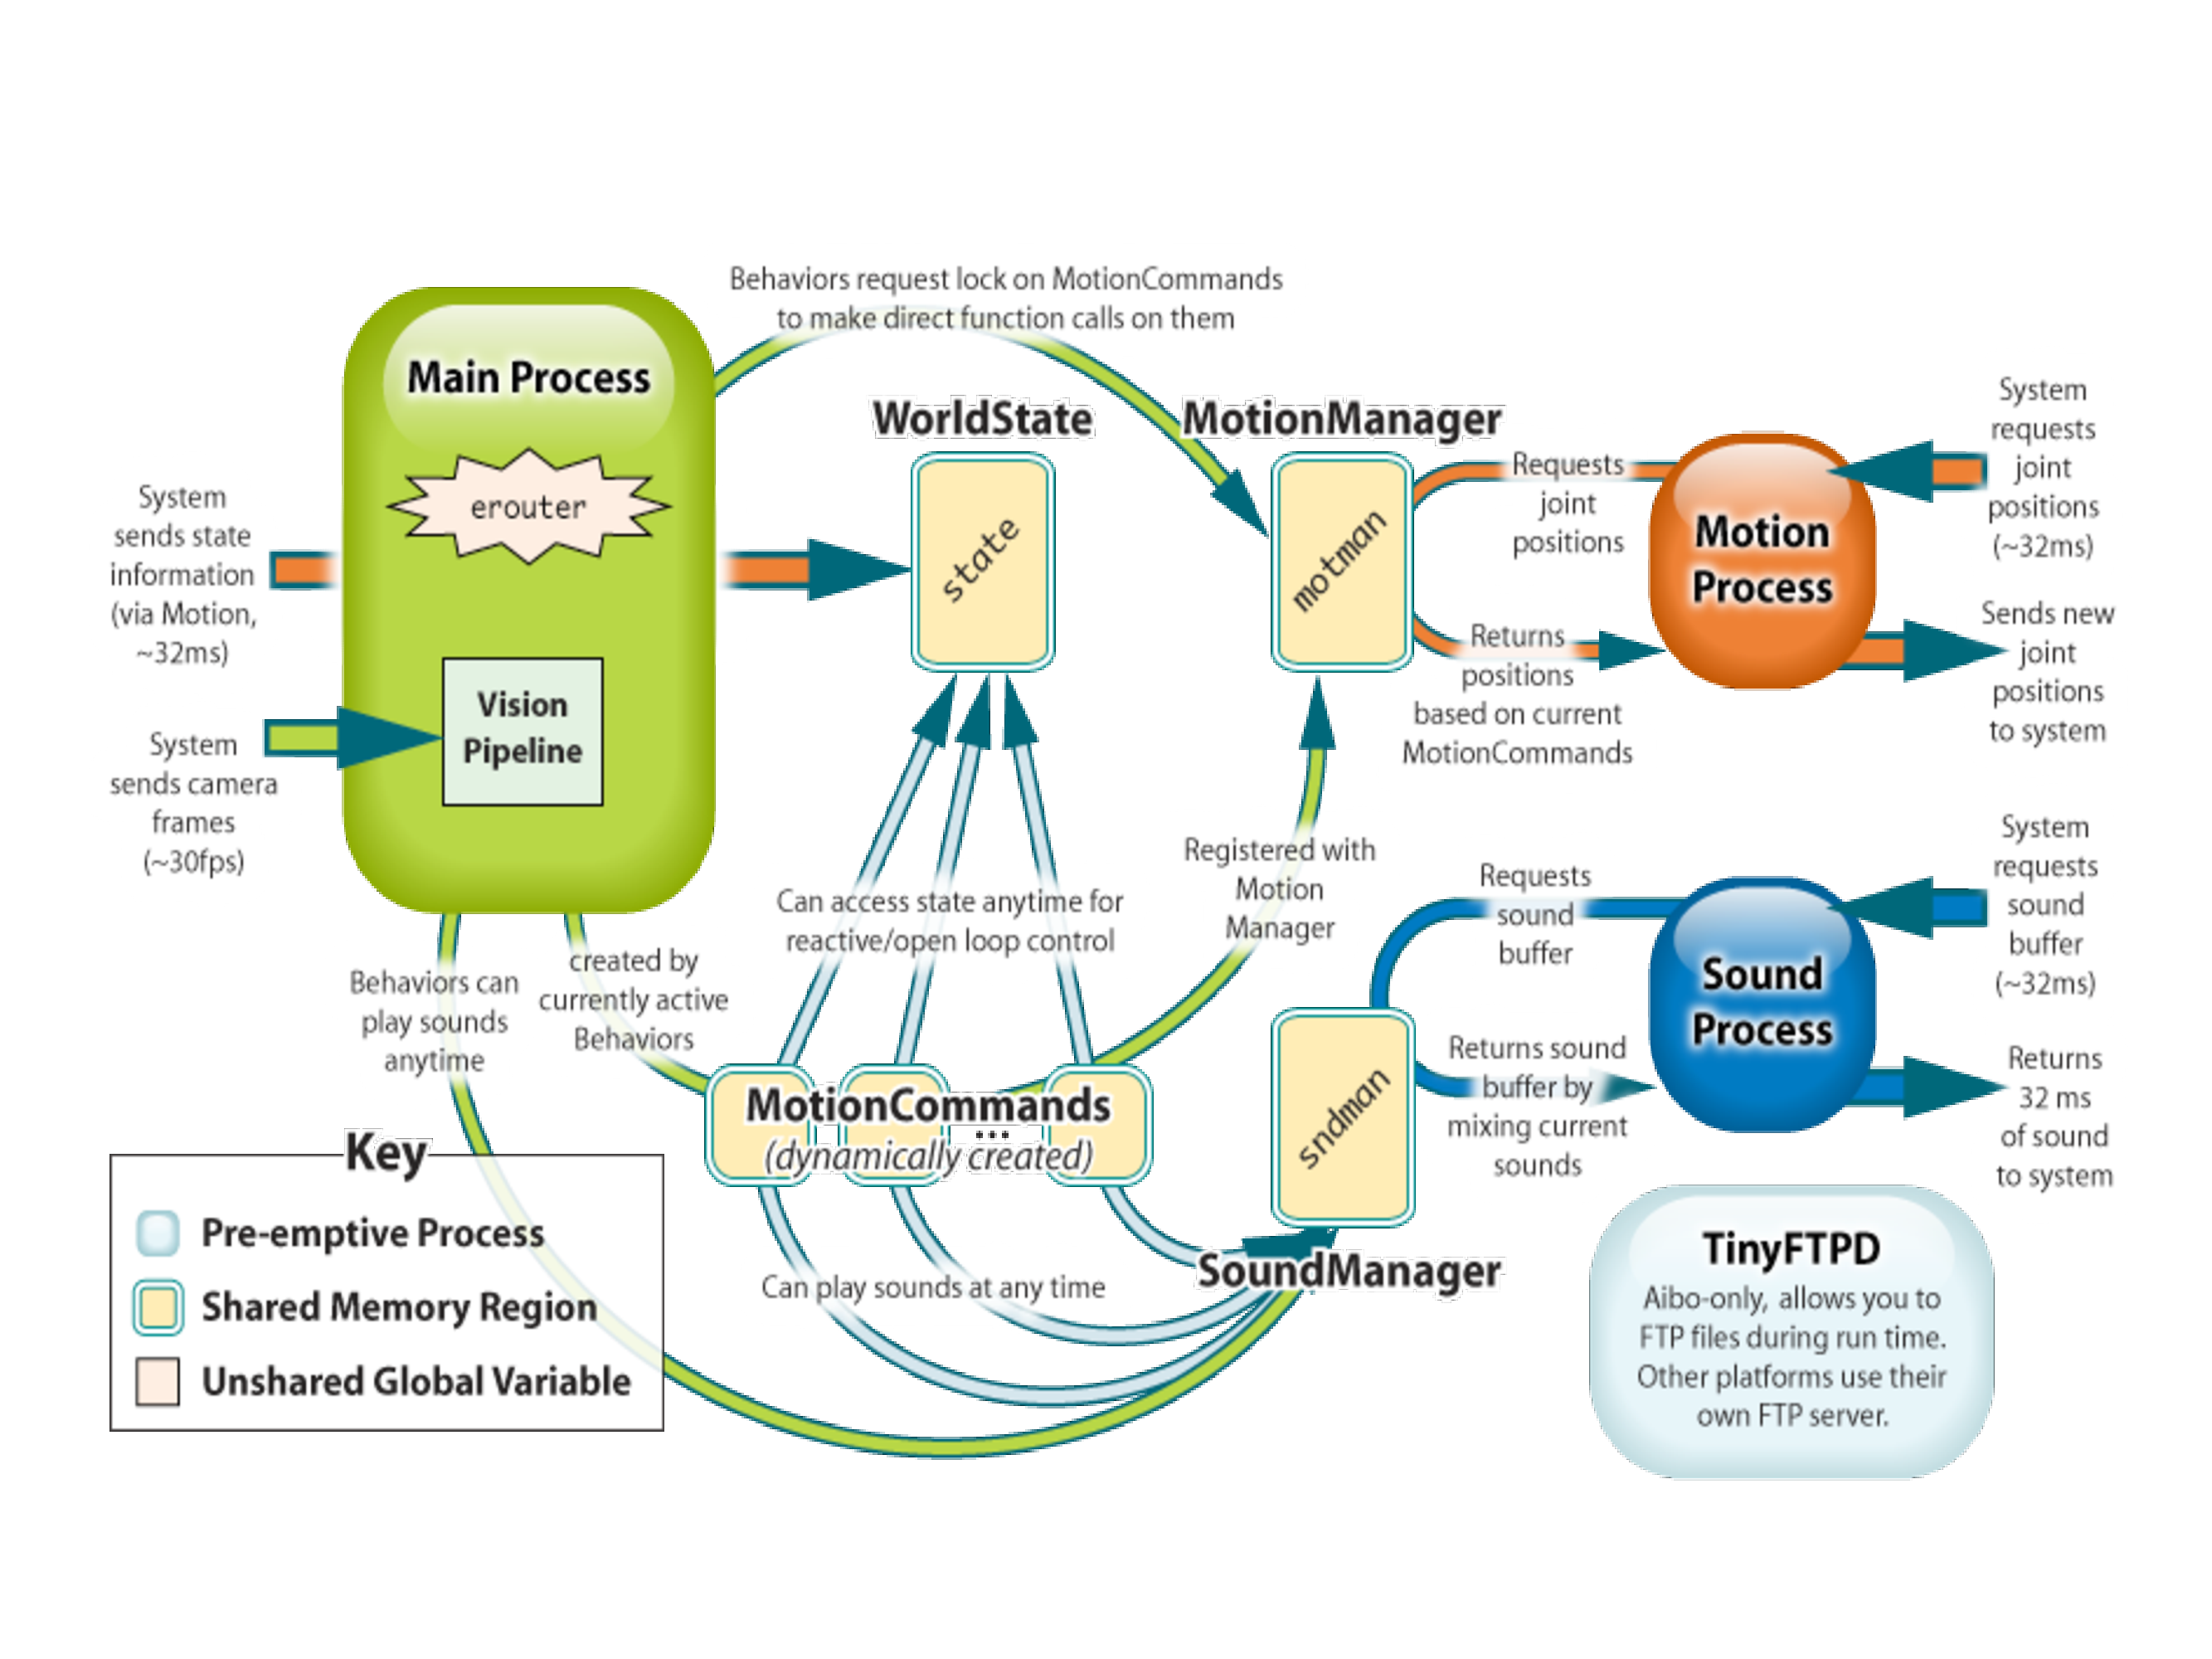
\includegraphics[scale=0.3]{images/tekkotsuarch.pdf}
	 \caption{Proceso de ejecución de un comportamiento en Tekkotsu.}
  \label{fig:tekkarch}
\end{figure}

\subsubsection{URBI}
\label{urbi}
URBI es el acrónimo de Universal Real-Time Behavior Interface y se trata de una plataforma de software libre para controlar y programar robots y sistemas automatizados en general. Algunos de los robots móviles que soporta URBI son AIBO, Bioloid, Mindstorm NXT, Pioneer, Wifibot o ARDrone \cite{urbi}.

URBI es un lenguaje basado en scripts de alto nivel con la ventaja que permite ejecutar comandos en paralelo. Existen dos formas de trabajar con URBI: La primera  se trata de usar el lenguaje de script con la intención de que este sea interpretado como un objeto de OPEN-R dentro de la tarjeta de memoria. La segunda consiste en una arquitectura cliente/servidor, donde el servidor es el AIBO, que permite enviar los scripts a través del terminal de URBI o bien enviar macros o ordenes concretas usando la libreria liburbi, Figura \ref{fig:urbiarc}. 

\begin{figure}[h!]
	\centering
    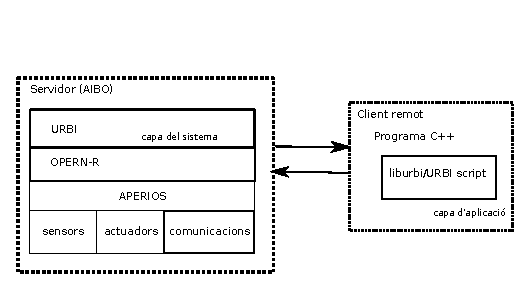
\includegraphics[scale=1.4]{images/urbiarc.pdf}
	 \caption{Arquitectura del AIBO con URBI.}
  \label{fig:urbiarc}
\end{figure}

La segunda opción abre varias vías de programación. Por un lado permite comunicarse por telnet y enviar comandos y por otro usar la librería liburbi que permite trabajar con C++, Java y Matlab

URBI permite y facilita el acceso a cada una de las articulaciones y sensores remotamente sin necesidad de implementar un servidor. Por ejemplo para consultar el valor de la articulación superior de la pierna izquierda se puede enviar el comando \texttt{legLF1.val;} y para asignarle un valor \texttt{legLF1.val=20;}\cite{urbicmd}.

\clearpage



\section{Comparación de alternativas para la programación}\label{seccomp}
Teniendo en cuenta la pretensión y objetivo final es poder programar AIBO con ROS se ha buscado la forma de atacar el problema desde todos los flancos. 
Una de ellas y completamente diferente a las demás ha sido buscar un punto de acceso al hardware con la intención de poder instalar alguna distribución de linux, lo que permitiría implementar el modulo de ROS de como un sistema embebido. Pero tras desmontar gran parte de las piezas solo se encontró un puerto que no coincidía con ningún estándar y se abandonó dicho camino.  

Solo queda usar una arquitectura cliente/servidor de forma que el modulo de ROS se ejecute en el cliente remoto, pero sea capaz adquirir de forma sencilla y rápida el estado del AIBO y a la vez actuar sobre el.


Se plantean tres posibilidades de programación: OPEN-R, Tekkotsu y URBI.
En los tres casos es imprescindible programar el cliente en el correspondiente lenguaje. Pero respeto al servidor URBI ahorraría tener que desarrollarlo puesto que el sistema operativo nos permite interactuar de forma remota. Tekkotsu permite interactuar de forma remota pero no hay ningun comportamiento que permita enviar ordenes a los actuadores y habría qu implementarlo. Por último con OPEN-R habría que implementar el servidor entero tanto el envió como la recepción. 
De todos modos se ha probado de instalar y establecer los tres marcos de trabajo y probado los tres lenguajes para comprobar su dificultad y su funcionamiento. Respeto a OPEN-R se ha encontrado muy poca documentación y el comienzo de su aprendizaje ha sido realmente duro tanto el lenguaje en si como la configuración de todos los archivos. Tekkotsu parece un lenguaje más sencillo y no necesita apenas configurar archivos pero la única documentación encontrada ha sido para la ultima versión que no se ha conseguido compilar dentro de la tarjeta de memoria. En cambio si se ha logrado con una versión más antigua, la nueva parece no ser compatible con el compilador de OPEN-R, y se han podido hacer algunas pruebas aunque sin documentación de la versión y habiendo cambiado bastante las funciones, ha implicado un gran esfuerzo. 
Por lo que URBI se refiere su uso es realmente sencillo des del terminal , se ha encontrado bastante documentación para el uso en modo script y algo menos para el uso de liburbi. El único problema que hay que tener en cuenta es que la librería liburbi 1.5, la más reciente que es compatible con  AIBO, no es compatible con un sistema linux de 64 bits. 

\begin{table}[H]
\begin{center}
\begin{tabulary}{\textwidth}{|p{5cm}|p{2.5cm}|p{2.5cm}|p{2.5cm}|}
\hline

& \textbf{OPEN-R}
& \textbf{Urbi} 
& \textbf{Tekkotsu} \\\hline
Necesidad de programar un servidor.
& Si
& No
& Si \\ \hline
Necesidad de programar un cliente.
& Si
& Si
& Si\\ \hline
Permite la consulta del estado por telnet.
& No
& Si
& Si\\ \hline
Permite accionar las articulaciones por telnet.
& No
& Si
& No\\ \hline
Dificultad de programación (0-5)
& 5
& 2 
& 3\\ \hline
Documentación (0-5)
& 2
& 3
& 1\\ \hline
Plataforma del PC.
& Windows/ Linux/ OS
& Windows/ Linux 32bits/ OS
& Linux\\ \hline
\end{tabulary}
\end{center}
\caption{Comparación entre lenguajes usados sobre AIBO\label{complleng}}
\end{table}

En vista de la Tabla \ref{complleng} y de lo anteriormente comentado se descarta usar Tekkotsu por haber encontrado muy poca documentación de la versión que ha podido ser compilada. Si bien seria OPEN-R sería una buena opción ya que es la capa mas baja de programación que se permite tocar su aprendizaje es realmente duro y posiblemente no habría tiempo de implementar el modulo deseado. Por lo tanto se partirá de URBI como lenguaje dado su fácil uso y que proporciona unas buenas herramientas para alcanzar el objetivo.


Partiendo del lenguaje URBI se plantean dos opciones de desarrollo:
\begin{itemize}
\item Usar liburbi con C++.
\item Usar un script de python que use la terminal de URBI bajo una conexión telnet.
\end{itemize}

Con tal de encontrar cual es la mejor opción se realizarán una serie de experimentos antes de implementar el paquete. 

\subsection{Lectura de datos}\label{compenvio}
En el primer experimento se valorará la velocidad de lectura de una sola variable del sistema y se cuantificará su frecuencia de refresco. Se ha usado para este experimento el valor de una articulación.

El procedimiento para adquirir los datos será el mostrado en la Figura \ref{fig:readleg}.


\begin{figure}[h!]
	\centering
    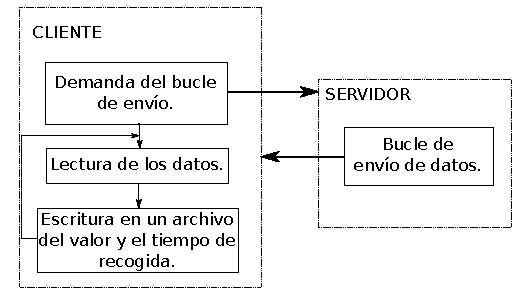
\includegraphics[scale=1.4]{images/lectdata.pdf}
	 \caption{Estructura de la lectura de una variable.}
  \label{fig:readleg}
\end{figure}

La escritura de los valores de la articulación y el tiempo se escriben en un archivo de texto para su posterior tratamiento.

El experimento consistirá en realizar la adquisición de datos durante 10 segundos y repetir el experimento 15 veces por método. La velocidad de envío estará limitada por el servidor ya que se le pide que envíe el refresco continuo de la variable.

\subsubsection{Método con liburbi y C++}

La estructura del programa es la que sigue\footnote{El script se puede encontrar en el Anexo \ref{getDataOneLegC++}}. 

\begin{itemize}
\item Inicialización del cliente URBI.
\item Inicialización del callback: Éste es llamado cada vez que se reciba un dato con la etiqueta asignada. 
\begin{itemize}
\item Se toma el valor de la variable (aunque no se necesaria para este experimento).
\item Se consulta el tiempo en que ha sido recibido el dato.
\item Se guarda el dato y el tiempo.
\end{itemize}
\item Demanda del bucle y asignación de una etiqueta.
\item Inicialización del archivo donde se guardarán los datos.
\item Ejecución del bucle de URBI: Se trata de una función que crea un bucle de comunicación cliente/servidor. 
\end{itemize}

\subsubsection{Método con telnet y python}
La idea de este script\footnote{Se puede consultar el scrript en el Anexo \ref{getDataOneLegPy}} es trabajar con la terminal de URBI, Figura \ref{fig:telnet},  mediante una conexión telnet.

\begin{figure}[h!]
	\centering
    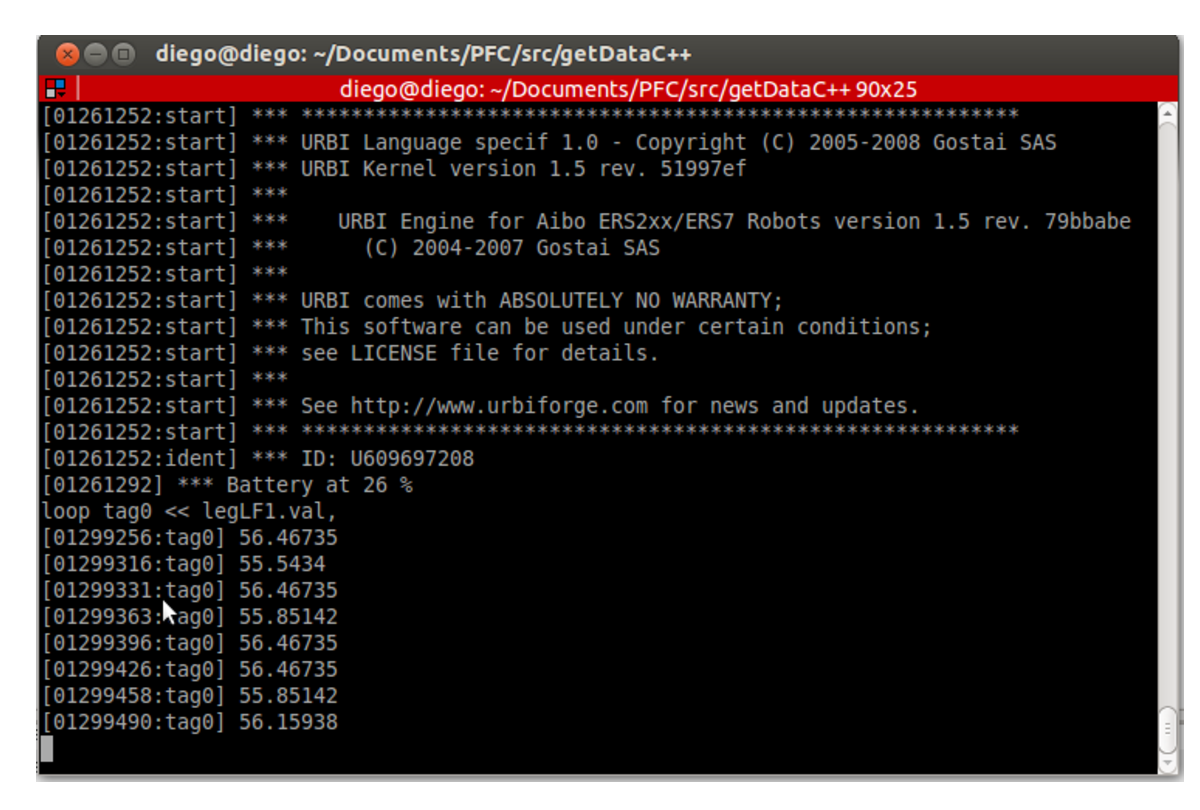
\includegraphics[scale=0.65]{images/telnet.pdf}
	 \caption{Terminal URBI consultando un dato.}
  \label{fig:telnet}
\end{figure}

La estructura del programa será parecida a la anterior:

\begin{itemize}
\item Inicialización del objeto telnet.
\item Lectura de la terminal y eliminación de la cabecera de URBI.
\item Escritura de la comanda para recibir el bucle  de envío. Para facilitar la lectura de los datos y diferenciar entre uno i el anterior se hace enviar una marca después de cada dato.
\item Bucle de lectura y escritura.
\begin{itemize}
\item Tratamiento de la lectura:
\begin{itemize}
\item Lectura hasta encontrar la marca la marca.
\item Eliminación de las cadenas cortadas por el envío de la información de la batería\footnote{Cada vez que la batería baja la carga se escribe el porcentaje restante por la terminal de URBI.}
\item Segmentación de la cadena para finalmente guardar sólo el valor.
\end{itemize}
\item Adquisición del tiempo.
\item Escritura del tiempo y el valor en el archivo de texto.
\end{itemize} 
\end{itemize}

\subsubsection{Comparación de los resultados}
%De los datos obtenidos de las 15 replicas de cada método se han hecho las diferencias de tiempos entre un dato y el siguiente y se ha echo el inverso de este intervalo con tal de obtener la frecuencia entre datos, se prefiere trabajar con el inverso debido a la comodidad de la escala.
De los datos obtenidos de las 15 replicas de cada método se han hecho las diferencias de tiempos entre un dato y el siguiente y se ha echo el inverso de este intervalo con tal de obtener la frecuencia entre datos.
\begin{figure}[H]
	\centering
\begin{tikzpicture}
\pgfplotsset{width=15cm,compat=1.10}
\begin{axis}[
enlargelimits=0.02,
xlabel={$Hz$},
y=0.6cm,
ytick={1,2,3,4,5,6,7,8,9,10,11,12,13,14,15,16,17,18,19,20,21,22,23,24,25,26,27,28,29,30},
yticklabels={Python 1, Python 2, Python 3,Python 4, Python 5,Python 6, Python 7, Python 8, Python 9, Python 10,Python 11,Python 12,Python 13,Python 14,Python 15,luburbi 1,luburbi 2,luburbi 3,luburbi 4,luburbi 5,luburbi 6,luburbi 7,luburbi 8,luburbi 9,luburbi 10,luburbi 11,luburbi 12,luburbi 13,luburbi 14,luburbi 15},
boxplot/variable width,
boxplot/draw direction=x,
]
\addplot [blue, mark=*, boxplot prepared={
lower whisker=0.68, lower quartile=31.34,
median=223.06,
upper quartile=3705.215, upper whisker=16710.37,}]
table[row sep=\\,y index=0] {
data\\ 2593.6 \\ 
};
coordinates {};
\addplot [blue,mark=*, boxplot prepared={
lower whisker=1.56, lower quartile=30.4,
median=33.07, upper quartile=3226.39,
upper whisker=12483}]
table[row sep=\\,y index=0] {
data\\ 1349.34 \\ 
};
coordinates {};
\addplot [blue,mark=*, boxplot prepared={
lower whisker=0.72, lower quartile=31.17,
median=78.39, upper quartile=3844.5,
upper whisker=14266.34}]
table[row sep=\\,y index=0] {
data\\ 2049.26 \\ 
};
coordinates {};
\addplot [blue,mark=*, boxplot prepared={
lower whisker=1.08, lower quartile=31.3,
median=83.9, upper quartile=3572.7,
upper whisker=8322}]
table[row sep=\\,y index=0] {
data\\ 1813.9 \\ 
};
coordinates {};
\addplot [blue,mark=*, boxplot prepared={
lower whisker=0.22, lower quartile=32.35,
median=3844.5, upper quartile=5882.6,
upper whisker=20068.4}]
table[row sep=\\,y index=0] {
data\\ 3371.85 \\ 
};
coordinates {};
\addplot [blue,mark=*, boxplot prepared={
lower whisker=0.28, lower quartile=31.24,
median=73.7, upper quartile=5555,
upper whisker=7145}]
table[row sep=\\,y index=0] {
data\\ 2473.14 \\ 
};
coordinates {};
\addplot [blue,mark=*, boxplot prepared={
lower whisker=1.67, lower quartile=30.46,
median=31.92, upper quartile=83.4,
upper whisker=11125.5}]
table[row sep=\\,y index=0] {
data\\ 871.16 \\ 
};
coordinates {};
\addplot [blue,mark=*, boxplot prepared={
lower whisker=0.71, lower quartile=2857.15,
median=3844.5, upper quartile=4346.5,
upper whisker=14266}]
table[row sep=\\,y index=0] {
data\\ 3253 \\ 
};
coordinates {};
\addplot [blue,mark=*, boxplot prepared={
lower whisker=1.06, lower quartile=35.83,
median=3449.3, upper quartile=4213.6,
upper whisker=16644}]
table[row sep=\\,y index=0] {
data\\ 3027 \\ 
};
coordinates {};
\addplot [blue,mark=*, boxplot prepared={
lower whisker=0.26, lower quartile=3332.1,
median=4549, upper quartile=9098,
upper whisker=14266}]
table[row sep=\\,y index=0] {
data\\ 5609 \\ 
};
coordinates {};
\addplot [blue,mark=*, boxplot prepared={
lower whisker=0.69, lower quartile=33,
median=3332.78, upper quartile=7696,
upper whisker=24966}]
table[row sep=\\,y index=0] {
data\\ 4460 \\ 
};
coordinates {};
\addplot [blue,mark=*, boxplot prepared={
lower whisker=0.8, lower quartile=31.7,
median=3334.1, upper quartile=4544.4,
upper whisker=16710}]
table[row sep=\\,y index=0] {
data\\ 3128.23 \\ 
};
coordinates {};
\addplot [blue,mark=*, boxplot prepared={
lower whisker=1.61, lower quartile=30.85,
median=32.6, upper quartile=3125,
upper whisker=14266}]
table[row sep=\\,y index=0] {
data\\ 1373.76 \\ 
};
coordinates {};
\addplot [blue,mark=*, boxplot prepared={
lower whisker=0.7, lower quartile=31.2,
median=64.25, upper quartile=3449.3,
upper whisker=14315}]
table[row sep=\\,y index=0] {
data\\ 1973.5 \\ 
};
coordinates {};
\addplot [blue,mark=*, boxplot prepared={
lower whisker=0.14, lower quartile=4346.4,
median=7695, upper quartile=11096,
upper whisker=12520.31}]
table[row sep=\\,y index=0] {
data\\ 2473.14 \\ 
};
coordinates {};
\addplot [mark=*, boxplot prepared={
lower whisker=0.8,
lower quartile=7696,
median=12520.3,
upper quartile=24966,
upper whisker=99864.38}]
table[row sep=\\,y index=0] {
data\\ 17220.7 \\ 
};
coordinates {};
\addplot [mark=*, boxplot prepared={
lower whisker=0.07,
lower quartile=7696,
median=24966,
upper quartile=33288.1,
upper whisker=33554.4}]
table[row sep=\\,y index=0] {
data\\ 19751.08 \\ 
};
coordinates {};
\addplot [mark=*, boxplot prepared={
lower whisker=0.9,
lower quartile=31.2,
median=34.59,
upper quartile=12492.4,
upper whisker=33554.4}]
table[row sep=\\,y index=0] {
data\\ 5478.22 \\ 
};
coordinates {};
\addplot [mark=*, boxplot prepared={
lower whisker=0.23,
lower quartile=9088,
median=24966,
upper quartile=12492.4,
upper whisker=33554.4}]
table[row sep=\\,y index=0] {
data\\ 20500 \\ 
};
coordinates {};
\addplot [mark=*, boxplot prepared={
lower whisker=0.16,
lower quartile=24966,
median=25115.6,
upper quartile=33288.1,
upper whisker=33554.4}]
table[row sep=\\,y index=0] {
data\\ 26177.7 \\ 
};
coordinates {};
\addplot [mark=*, boxplot prepared={
lower whisker=0.06,
lower quartile=24966,
median=24966,
upper quartile=33288.1,
upper whisker=33554.4}]
table[row sep=\\,y index=0] {
data\\ 25822.2 \\ 
};
coordinates {};
\addplot [mark=*, boxplot prepared={
lower whisker=0.88,
lower quartile=32.66,
median=14266,
upper quartile=19972.8,
upper whisker=50533.8}]
table[row sep=\\,y index=0] {
data\\ 15288.8 \\ 
};
coordinates {};
\addplot [mark=*, boxplot prepared={
lower whisker=4.2,
lower quartile=30.4,
median=31.7,
upper quartile=38.77,
upper whisker=16710.4}]
table[row sep=\\,y index=0] {
data\\ 1827 \\ 
};
coordinates {};
\addplot [mark=*, boxplot prepared={
lower whisker=1.2,
lower quartile=31.7,
median=9098.3,
upper quartile=20068.4,
upper whisker=99864.38}]
table[row sep=\\,y index=0] {
data\\ 11732.4 \\ 
};
coordinates {};
\addplot [mark=*, boxplot prepared={
lower whisker=1.2,
lower quartile=31.35,
median=7413.6,
upper quartile=24966,
upper whisker=33554.4}]
table[row sep=\\,y index=0] {
data\\ 11941.8 \\ 
};
coordinates {};
\addplot [mark=*, boxplot prepared={
lower whisker=0.8,
lower quartile=31.2,
median=44.9,
upper quartile=33288,
upper whisker=102300}]
table[row sep=\\,y index=0] {
data\\ 20545 \\ 
};
coordinates {};
\addplot [mark=*, boxplot prepared={
lower whisker=0.9,
lower quartile=30.9,
median=31.86,
upper quartile=5882.6,
upper whisker=33554.4}]
table[row sep=\\,y index=0] {
data\\ 4640 \\ 
};
coordinates {};
\addplot [mark=*, boxplot prepared={
lower whisker=1.13,
lower quartile=30.9,
median=31.8,
upper quartile=139.47,
upper whisker=99864.4}]
table[row sep=\\,y index=0] {
data\\ 4520.6 \\ 
};
coordinates {};
\addplot [mark=*, boxplot prepared={
lower whisker=1.65,
lower quartile=31.8,
median=31.94,
upper quartile=8111.9,
upper whisker=102300}]
table[row sep=\\,y index=0] {
data\\ 10729 \\ 
};
coordinates {};
\addplot [mark=*, boxplot prepared={
lower whisker=1.64,
lower quartile=31.11,
median=33.44,
upper quartile=24966,
upper whisker=33554.4}]
table[row sep=\\,y index=0] {
data\\ 8990 \\ 
};
coordinates {};
\end{axis}
\end{tikzpicture}
 \caption{Diagrama de cajas de la frecuencia de datos para las 15 replicas de cada método.}
  \label{fig:OneLegBox}
\end{figure}


El gráfico de la Figura \ref{fig:OneLegBox} muestra como claramente al trabajar con liburbi se obtienen medias más altas en la mayoría de replicas y de la misma manera gran parte de los datos se envían más rápido. Aun así los valores mínimos parecen muy similares y la variabilidad es mucho mayor con liburbi, echo que no interesa.

Es interesante observar los mínimos de cada serie en más detalle pues nos indican cuan largos son los bloqueos que se producen y si existe alguna diferencia entre ambos programas, Figura \ref{fig:MinOneLeg}.
Si bien parece que liburbi tiene una tendencia a tener unos mínimos más bajos se ha realizado un análisis sobre la varianza (ANOVA) de los mínimos. Los resultados han sido que con intervalo de confianza del 95\% no se puede afirmar con un p-valor de 0.4 que los valores provengan de distintas poblaciones.
 

\begin{figure}[H]
	\centering
    \begin{tikzpicture}
    \usetikzlibrary{patterns}
    \pgfplotsset{width=15cm,compat=1.10}

\begin{axis}[
x tick label style={
/pgf/number format/1000 sep=},
xlabel=replicas,
ylabel=Hz,
enlargelimits=0.08,
legend style={at={(0.5,-0.15)},
anchor=north,legend columns=-1},
ybar=0.1pt,% configures `bar shift'
bar width=10pt,
]
\addplot [draw=black,pattern=horizontal lines dark blue]
coordinates {(1,0.675) (2,1.561)
(3,0.72) (4,1.079 ) (5,0.217 ) (6,0.276) (7,1.67) (8,0.714) (9,1.064 ) (10,0.264 ) (11,0.696 ) (12,1.618 ) (13,0.8 ) (14,0.7 ) (15,0.135 ) };
\addplot [draw=blue,pattern=horizontal lines light blue]
coordinates {(1,0.8) (2,0.074)
(3,0.9) (4,0.234 ) (5,0.155 ) (6,0.06 ) (7,0.883 ) (8,4.239 ) (9,1.2 ) (10,1.2 ) (11,0.8 ) (12,1.133 ) (13,1.659 ) (14,1.636 ) (15,0.933 )};
\legend{python,liburbi}
\end{axis}
\end{tikzpicture}
	 \caption{Mínimos de la frecuencia en les 15 repliques de los dos métodos.}
  \label{fig:MinOneLeg}
\end{figure}
Por otro lado se ha observado, no la durada de estos pequeños bloqueos sino la cuantos se producen en cada caso. Para ello se ha realizado un gráfico donde se clasifican unos intervalos de frecuencias. 
\begin{itemize}
\item Menor que 0.5 Hz: Este intervalos se consideran bloqueos y son los menos deseados.
\item De 0.5 a 5 Hz: No se consideran bloqueos pero es una frecuencia demasiado baja para trabajar de forma remota con un robot móvil.
\item De 5 a 10Hz: Se trata de una velocidad aceptable.
\item Mayor que 10: Se considera la frecuencia de trabajo ideal.
\end{itemize}

\begin{figure}[H]
	\centering
    \begin{tikzpicture}
    \usetikzlibrary{patterns}
    \pgfplotsset{width=15cm,compat=1.10}

\begin{axis}[
ybar,
ylabel=Hz,
bar width=30pt,
enlargelimits=0.15,
legend style={at={(0.5,-0.15)},
anchor=north,legend columns=-1},
symbolic x coords={menor que 0.5,entre 0.5 y 5,entre 5 y 10,mayor que 10},
xtick=data,
]

\addplot [draw=blue,pattern=horizontal lines light blue] coordinates {(menor que 0.5, 4) (entre 0.5 y 5, 126) (entre 5 y 10, 152) (mayor que 10,4511)};
\addplot [draw=black,pattern=horizontal lines dark blue] coordinates {(menor que 0.5,5) (entre 0.5 y 5,99) (entre 5 y 10,217) (mayor que 10,4132)};
\legend{python, liburbi}
\end{axis}
\end{tikzpicture}
	 \caption{Histograma de la frecuencia en les 15 repliques de los dos métodos.}
  \label{fig:histLeg}
\end{figure}

La gran mayoría de los datos, según la Figura \ref{fig:histLeg}, se encuentran en la zona de frecuencias deseadas y ambos métodos tienen un comportamiento muy parecido. En la franja considerada como bloqueos, en las 15 replicas que equivaldrían a unos 150 segundos de funcionamiento, se han dado 4 casos en liburbi y 5 en python.   



A la vista de los resultados obtenidos se a querido comprobar como afecta la cantidad de datos a enviar en el tiempo de recepción. Para ello se a realizado el mismo experimento pero leyendo todas las articulaciones en vez de solo una.

\begin{figure}[H]
	\centering
   	\begin{tikzpicture}
\pgfplotsset{width=15cm,compat=1.10}
\begin{axis}[
enlargelimits=0.02,
xlabel={$Hz$},
y=0.6cm,
ytick={1,2,3,4,5,6,7,8,9,10,11,12,13,14,15,16,17,18,19,20,21,22,23,24,25,26,27,28,29,30},
yticklabels={Python 1, Python 2, Python 3,Python 4, Python 5,Python 6, Python 7, Python 8, Python 9, Python 10,Python 11,Python 12,Python 13,Python 14,Python 15,luburbi 1,luburbi 2,luburbi 3,luburbi 4,luburbi 5,luburbi 6,luburbi 7,luburbi 8,luburbi 9,luburbi 10,luburbi 11,luburbi 12,luburbi 13,luburbi 14,luburbi 15},
boxplot/variable width,
boxplot/draw direction=x,
]
\addplot [blue, mark=*, boxplot prepared={
lower whisker=8.29, lower quartile=10010.3,
median=11125,
upper quartile=12483, upper whisker=50533.8,}]
table[row sep=\\,y index=0] {
data\\ 11570.5 \\ 
};
coordinates {};
\addplot [blue,mark=*, boxplot prepared={
lower whisker=3.88, lower quartile=9986,
median=11125, upper quartile=12520.3,
upper whisker=99864.4}]
table[row sep=\\,y index=0] {
data\\ 14287.8 \\ 
};
coordinates {};
\addplot [blue,mark=*, boxplot prepared={
lower whisker=0.8, lower quartile=11096,
median=12483, upper quartile=25115.6,
upper whisker=99864.4}]
table[row sep=\\,y index=0] {
data\\ 17289.2 \\ 
};
coordinates {};
\addplot [blue,mark=*, boxplot prepared={
lower whisker=0.74, lower quartile=11096,
median=11125.5, upper quartile=24966,
upper whisker=50533.8}]
table[row sep=\\,y index=0] {
data\\ 16558.8 \\ 
};
coordinates {};
\addplot [blue,mark=*, boxplot prepared={
lower whisker=0.48, lower quartile=10010.3,
median=11125, upper quartile=33288,
upper whisker=99864}]
table[row sep=\\,y index=0] {
data\\ 17471 \\ 
};
coordinates {};
\addplot [blue,mark=*, boxplot prepared={
lower whisker=0.7, lower quartile=11096,
median=12520, upper quartile=33288,
upper whisker=102300}]
table[row sep=\\,y index=0] {
data\\ 19609 \\ 
};
coordinates {};
\addplot [blue,mark=*, boxplot prepared={
lower whisker=0.69, lower quartile=11096,
median=12520, upper quartile=33288,
upper whisker=99864}]
table[row sep=\\,y index=0] {
data\\ 19857 \\ 
};
coordinates {};
\addplot [blue,mark=*, boxplot prepared={
lower whisker=0.74, lower quartile=11096,
median=12483, upper quartile=33288,
upper whisker=99864}]
table[row sep=\\,y index=0] {
data\\ 18635 \\ 
};
coordinates {};
\addplot [blue,mark=*, boxplot prepared={
lower whisker=7.45, lower quartile=9986,
median=11125, upper quartile=12520,
upper whisker=102300}]
table[row sep=\\,y index=0] {
data\\ 13574 \\ 
};
coordinates {};
\addplot [blue,mark=*, boxplot prepared={
lower whisker=0.99, lower quartile=10010,
median=11125, upper quartile=16644,
upper whisker=50533}]
table[row sep=\\,y index=0] {
data\\ 15703 \\ 
};
coordinates {};
\addplot [blue,mark=*, boxplot prepared={
lower whisker=0.73, lower quartile=10010,
median=11125, upper quartile=25115,
upper whisker=50533}]
table[row sep=\\,y index=0] {
data\\ 17033 \\ 
};
coordinates {};
\addplot [blue,mark=*, boxplot prepared={
lower whisker=0.71, lower quartile=11096,
median=12483, upper quartile=33288,
upper whisker=50533}]
table[row sep=\\,y index=0] {
data\\ 17844 \\ 
};
coordinates {};
\addplot [blue,mark=*, boxplot prepared={
lower whisker=0.66, lower quartile=11096,
median=12483, upper quartile=33288,
upper whisker=50533}]
table[row sep=\\,y index=0] {
data\\ 17976 \\ 
};
coordinates {};
\addplot [blue,mark=*, boxplot prepared={
lower whisker=0.79, lower quartile=11096,
median=11125, upper quartile=25115,
upper whisker=50533}]
table[row sep=\\,y index=0] {
data\\ 16835 \\ 
};
coordinates {};
\addplot [blue,mark=*, boxplot prepared={
lower whisker=0.65, lower quartile=11096,
median=11125, upper quartile=24966,
upper whisker=50353}]
table[row sep=\\,y index=0] {
data\\ 16723 \\ 
};
coordinates {};
\addplot [mark=*, boxplot prepared={
lower whisker=0.77,
lower quartile=16710,
median=24966,
upper quartile=33288,
upper whisker=99864.38}]
table[row sep=\\,y index=0] {
data\\ 25651 \\ 
};
coordinates {};
\addplot [mark=*, boxplot prepared={
lower whisker=0.63,
lower quartile=19972,
median=24966,
upper quartile=33288,
upper whisker=102300}]
table[row sep=\\,y index=0] {
data\\ 31444 \\ 
};
coordinates {};
\addplot [mark=*, boxplot prepared={
lower whisker=24.9,
lower quartile=19972,
median=24966,
upper quartile=33288,
upper whisker=33554}]
table[row sep=\\,y index=0] {
data\\ 22681 \\ 
};
coordinates {};
\addplot [mark=*, boxplot prepared={
lower whisker=0.74,
lower quartile=16644,
median=24966,
upper quartile=24966,
upper whisker=50533}]
table[row sep=\\,y index=0] {
data\\ 21260 \\ 
};
coordinates {};
\addplot [mark=*, boxplot prepared={
lower whisker=0.75,
lower quartile=16644,
median=24966,
upper quartile=33288,
upper whisker=99864.38}]
table[row sep=\\,y index=0] {
data\\ 24103 \\ 
};
coordinates {};
\addplot [mark=*, boxplot prepared={
lower whisker=0.74,
lower quartile=16644,
median=24966,
upper quartile=25115,
upper whisker=102300}]
table[row sep=\\,y index=0] {
data\\ 23236 \\ 
};
coordinates {};
\addplot [mark=*, boxplot prepared={
lower whisker=0.74,
lower quartile=16644,
median=24966,
upper quartile=25115,
upper whisker=50533}]
table[row sep=\\,y index=0] {
data\\ 22662 \\ 
};
coordinates {};
\addplot [mark=*, boxplot prepared={
lower whisker=10.22,
lower quartile=19972,
median=24966,
upper quartile=25115,
upper whisker=102300}]
table[row sep=\\,y index=0] {
data\\ 22105 \\ 
};
coordinates {};
\addplot [mark=*, boxplot prepared={
lower whisker=3.95,
lower quartile=19972,
median=24966,
upper quartile=25115,
upper whisker=33554}]
table[row sep=\\,y index=0] {
data\\ 22263 \\ 
};
%TOCA EL 10
coordinates {};
\addplot [mark=*, boxplot prepared={
lower whisker=0.75,
lower quartile=19972,
median=24966,
upper quartile=25115.6,
upper whisker=50533.8}]
table[row sep=\\,y index=0] {
data\\ 22365 \\ 
};
coordinates {};
\addplot [mark=*, boxplot prepared={
lower whisker=0.75,
lower quartile=16710,
median=24966,
upper quartile=33288,
upper whisker=99864}]
table[row sep=\\,y index=0] {
data\\ 24890 \\ 
};
coordinates {};
\addplot [mark=*, boxplot prepared={
lower whisker=0.74,
lower quartile=16644,
median=24966,
upper quartile=25115.6,
upper whisker=50533}]
table[row sep=\\,y index=0] {
data\\ 21865.6 \\ 
};
coordinates {};
\addplot [mark=*, boxplot prepared={
lower whisker=8.17,
lower quartile=20068,
median=24966,
upper quartile=25115,
upper whisker=99864.4}]
table[row sep=\\,y index=0] {
data\\ 23023.8 \\ 
};
coordinates {};
\addplot [mark=*, boxplot prepared={
lower whisker=0.78,
lower quartile=16644,
median=24966,
upper quartile=25115.6,
upper whisker=99864}]
table[row sep=\\,y index=0] {
data\\ 21991 \\ 
};
coordinates {};
\addplot [mark=*, boxplot prepared={
lower whisker=1.16,
lower quartile=16644,
median=24966,
upper quartile=33288,
upper whisker=102300}]
table[row sep=\\,y index=0] {
data\\ 23439 \\ 
};
coordinates {};
\end{axis}
\end{tikzpicture}
	 \caption{Diagrama de cajas de la frecuencia de datos para las 15 replicas de cada método con todas las articulaciones.}
  \label{fig:JointsBox}
\end{figure}

Bajo este experimento, Figura \ref{fig:JointsBox}, ambas distribuciones son más parecidas aunque se puede distinguir la tendencia a obtener valores más altos del método con liburbi.

\begin{figure}[H]
	\centering
\begin{tikzpicture}[baseline]
\pgfplotsset{width=8cm,compat=1.10}
\begin{axis}[
title=Python,
xlabel={$replicas$},
ylabel={$Hz$},
minor y tick num=1,
legend style={at={(0.5,-0.25)},
anchor=north,legend columns=-1},
]
\addplot[blue, only marks] table {data/mediaPyOne.dat};
\addplot[black, only marks] table {data/mediaPyAll.dat};
\addplot[black,sharp plot,update limits=false]
coordinates {(0,16731.4) (16,16731.4)};

\addplot[blue,sharp plot,update limits=false]
coordinates {(0,2999.5) (16,2999.5)};

\legend{un valor, todos los valores}
\end{axis}
\end{tikzpicture}
\begin{tikzpicture}[baseline]
\pgfplotsset{width=8cm,compat=1.10}
\begin{axis}[
title=liburbi,
xlabel={$replicas$},
ylabel={$Hz$},
minor y tick num=1,
]
\addplot[blue, only marks] table {data/mediaC++One.dat};
\addplot[black, only marks] table {data/mediaC++All.dat};
\addplot[black,sharp plot,update limits=false]
coordinates {(0,23532.4) (16,23532.4)};

\addplot[blue,sharp plot,update limits=false]
coordinates {(0,13611) (16,13611)};


\end{axis}
\end{tikzpicture}
	 \caption{Medias de las frecuencias de envío, comparando una el obtener el valor de una articulación con obtener el valor de todas las articulaciones.}
  \label{fig:compAllOne}
\end{figure}
La velocidad de envío es significativamente más alta en ambos casos aunque en el caso de python se muestra mas evidente Figura \ref{fig:compAllOne}. Una explicación es que el conjunto de valores se envíe como un solo paquete, en ese caso se está midiendo la frecuencia a la que las variables están disponibles, que a fin de cuentas es lo que realmente importa dado que se va a trabajar con ellas. Al parecer ante este echo responde mejor la lectura del terminal con python que no la adquisición mediante el callback de liuburbi. De todos modos se ha podido comprobar que la cantidad de variables a enviar no tiene un efecto negativo en las frecuencias medias.

Poniendo la atención en los bloqueos, Figuras \ref{fig:MinAllLeg} y \ref{fig:histAllLeg}, se puede asegurar el mismo comportamiento que en el experimento anterior. 
\newpage
    \begin{figure}[H]
	\centering
    \begin{tikzpicture}
\usetikzlibrary{patterns}
\pgfplotsset{width=11cm,compat=1.10}

\begin{axis}[
x tick label style={
/pgf/number format/1000 sep=},
xlabel=replicas,
ylabel=Hz,
enlargelimits=0.08,
legend style={at={(0.5,-0.15)},
anchor=north,legend columns=-1},
ybar=0.1pt,% configures `bar shift'
bar width=6pt,
]
\addplot [draw=black,pattern=horizontal lines dark blue]
coordinates {(1,8.29) (2,3.88)
(3,0.88) (4,0.74 ) (5,0.46 ) (6,0.69) (7,0.62) (8,0.744) (9,7.455 ) (10,0.995 ) (11,0.738 ) (12,0.713 ) (13,0.66 ) (14,0.792 ) (15,0.658 ) };
\addplot [draw=blue,pattern=horizontal lines light blue]
coordinates {(1,0.77) (2,0.63)
(3,24.98) (4,0.745 ) (5,0.759 ) (6,0.737 ) (7,0.745 ) (8,10.23 ) (9,3.953 ) (10,0.751 ) (11,0.753 ) (12,0.742 ) (13,8.173 ) (14,1.161 ) (15,0.933 )};
\legend{python,liburbi}
\end{axis}
\end{tikzpicture}

	 \caption{Mínimos de la frecuencia en les 15 repliques de los dos métodos.}
  \label{fig:MinAllLeg}
\end{figure}
\begin{figure}[H]
	\centering
\begin{tikzpicture}
    \usetikzlibrary{patterns}
    \pgfplotsset{width=11cm,compat=1.10}

\begin{axis}[
ybar,
ylabel=Hz,
bar width=30pt,
enlargelimits=0.15,
legend style={at={(0.5,-0.15)},
anchor=north,legend columns=-1},
symbolic x coords={menor que 0.5,entre 0.5 y 5,entre 5 y 10,mayor que 10},
xtick=data,
]

\addplot [draw=blue,pattern=horizontal lines light blue] coordinates {(menor que 0.5, 1) (entre 0.5 y 5, 38) (entre 5 y 10, 157) (mayor que 10,84283)};
\addplot [draw=black,pattern=horizontal lines dark blue] coordinates {(menor que 0.5,0) (entre 0.5 y 5,35) (entre 5 y 10,37) (mayor que 10,79348)};
\legend{python, liburbi}
\end{axis}
\end{tikzpicture}
 \caption{Histograma de la frecuencia en les 15 repliques de los dos métodos.}
  \label{fig:histAllLeg}
\end{figure}


\subsection{Envío de datos}\label{secenvdades}
Vista una de los sentidos de comunicación el siguiente experimento se va a fijar en el otro, el envió de los valores de las articulaciones del cliente al servidor con tal de controlar al AIBO.
El experimento consiste en enviar una trayectoria punto a punto a una articulación y comprobar que tal responde. La trayectoria será sinusoidal sin importar el periodo. Para valorar los resultados se leerá la respuesta de la articulación usando los módulos de lectura del experimento anterior, que condicionaran el resultado por sus errores y limitaciones. 

En este caso se ha contado con 3 opciones a comparar. Dado que por la terminal de URBI usando el cliente telnet no se ha permitió hacer la lectura y la escritura a la vez se ha tenido que hacer con dos clientes telnet. Esto ha planteado la duda si en liburbi tenia algún efecto el hecho de escribir y leer a la vez por el mismo cliente aunque este lo permita. Por este motivo se han planteado los siguientes programas:
\begin{itemize}
\item Python con un cliente telnet para lectura y otro para escritura.
\item C++ con un cliente URBI tanto para lectura como para escritura.
\item C++ con un cliente URBI para lectura y otro para escritura
\end{itemize}

En el desarrollo de los tres programas ha habido dos hechos a tener en cuenta y de destacada importancia.
Ha sido necesario la creación de un hilo de ejecución en paralelo con tal de tener dos bucles independientes dentro del cliente, el bucle de URBI y el de envío.
Por otro lado se ha investigado y experimentado con los modos de tratamiento  de ordenes que tiene URBI:
\begin{itemize}
\item \texttt{normal}: Es el modo por defecto. En caso de conflicto la ultima asignación tiene prioridad, pero en caso de que la ultima acabe la anterior toma el relevo.
\item \texttt{mix}: En caso de conflicto el valor asignado es una media de los valores en conflicto.
\item \texttt{add}: El valor asignado es la suma de los valores en conflicto.
\item \texttt{queue}: se forma un cola de entrada que se resuelve con un sistema FIFO (First In First Out).
\item \texttt{discard}: En caso de conflicto el valor de la variable no se modifica.
\item \texttt{cancel}: La ultima asignación toma prioridad y las anteriores son canceladas. 
\end{itemize}

Tras varias pruebas se ha decidido que el modo más conveniente para la implementación del modulo es el modo \texttt{cancel}.

El experimento\footnote{Los codigos se puede encontrar en los Anexos \ref{sinC} y \ref{sinP}} se ha realizado varias veces cambiando la frecuencia a la que se envían los puntos de la trayectoria. Se ha realizado a 1, 2, 5 y 10 Hz, no se ha enviado a mas velocidad ya que el movimiento a una frecuencia de mas de 10 Hz era inconstante y poco suave.
Se han descartado los experimentos en que se ha producido un bloqueo.
 
\begin{figure}[H]
	\centering
    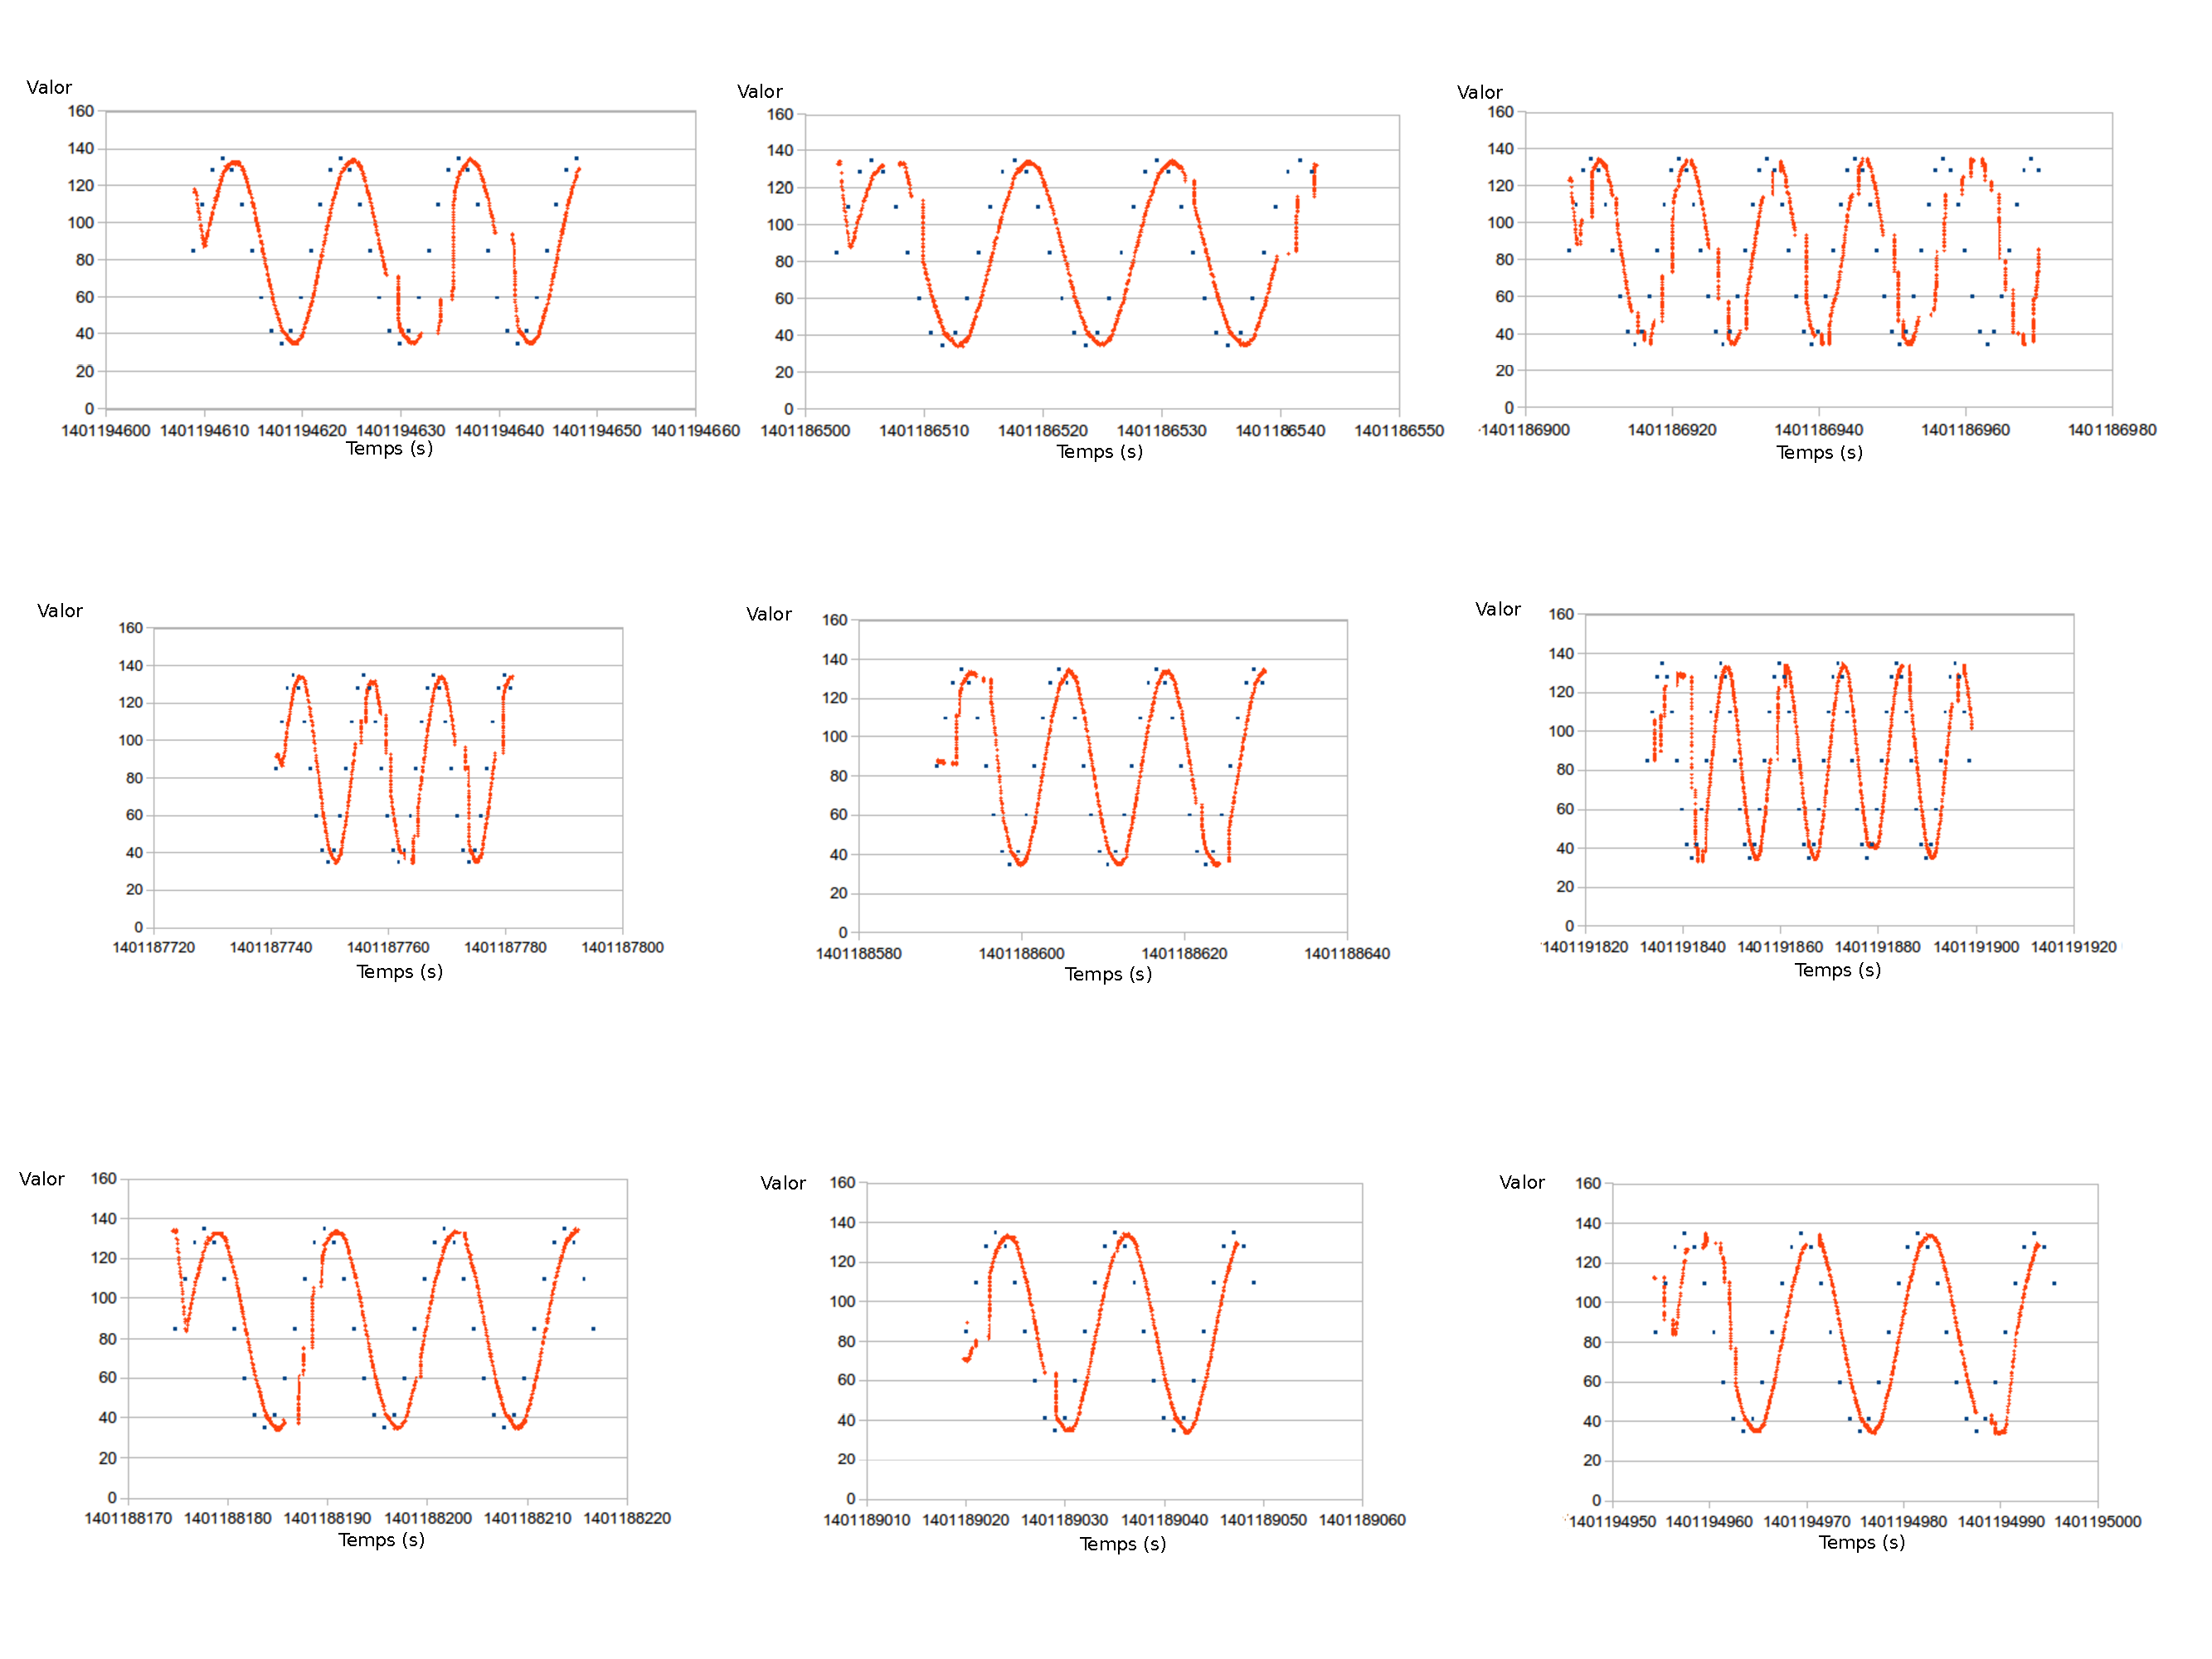
\includegraphics[scale=0.37]{images/sin1H.pdf}
	 \caption{En azul está graficado las posiciones enviadas a 1Hz y en rojo las lecturas. En columnas se encuentran las replicas del mismo método y por filas los tres métodos usados, en orden descendente son liburbi con un cliente, liburbi con dos cliente y python.}
  \label{fig:sin1H}
\end{figure}
\begin{figure}[H]
	\centering
    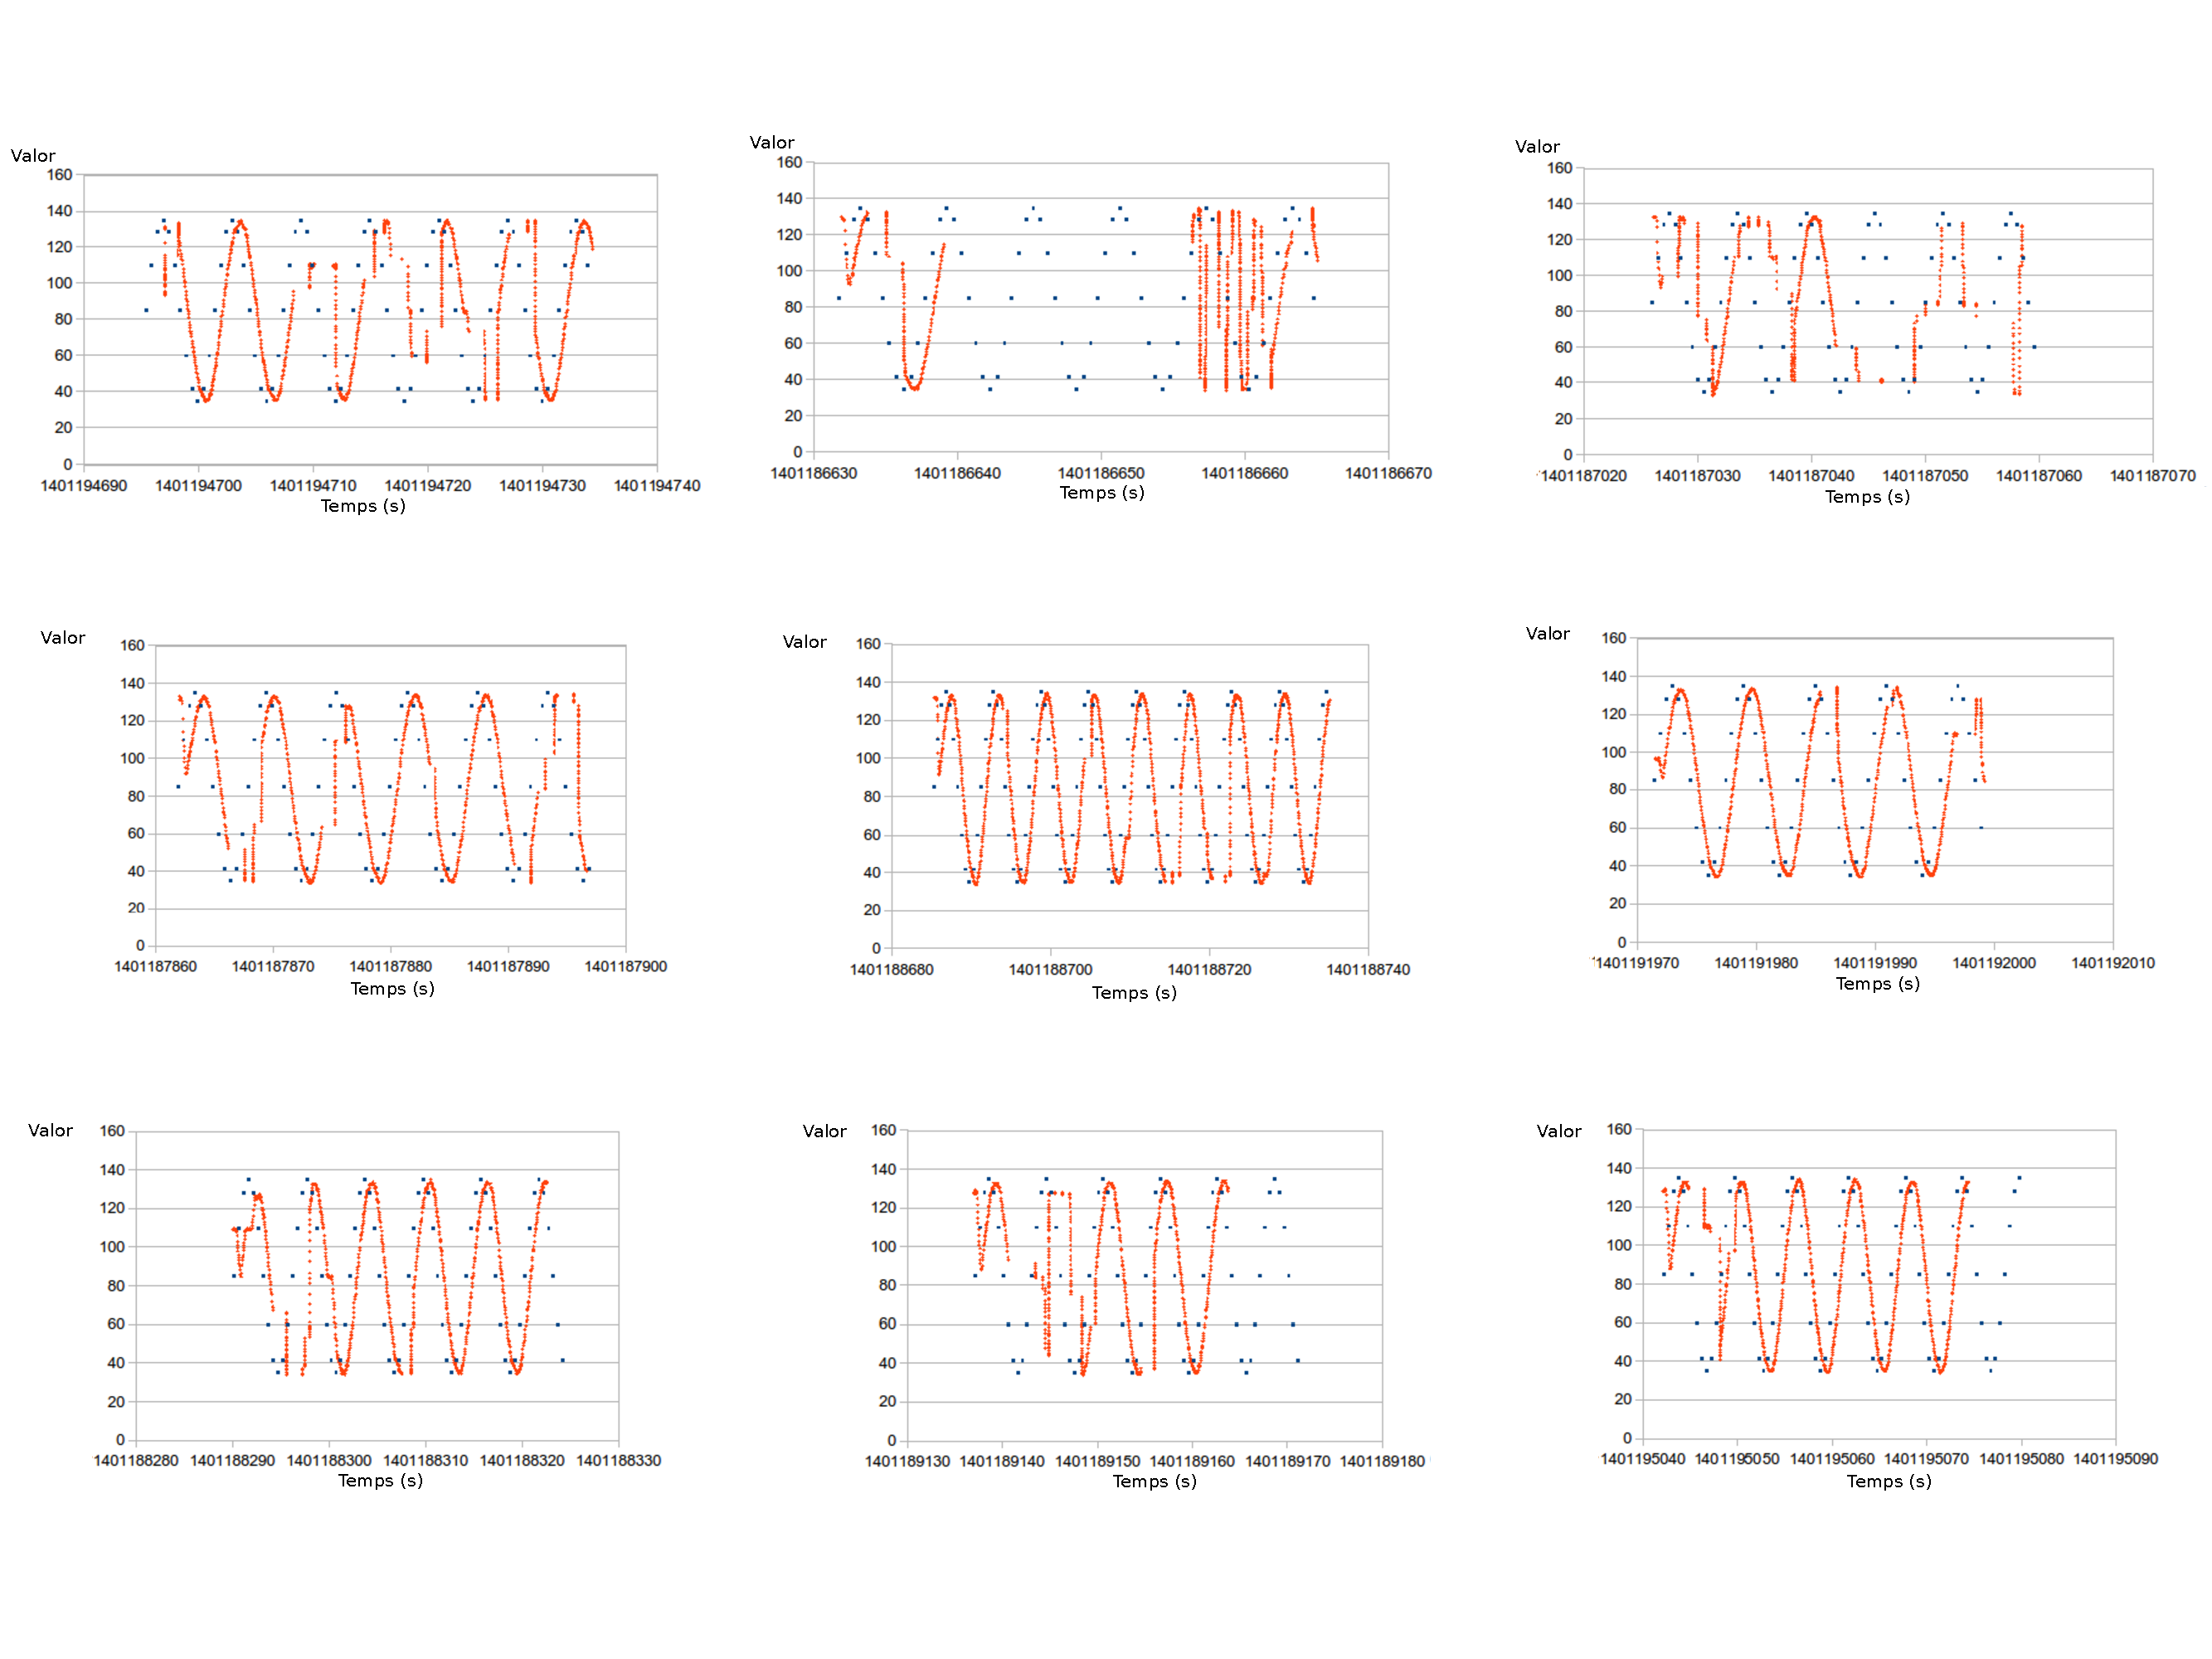
\includegraphics[scale=0.37]{images/sin2H.pdf}
	 \caption{En azul está graficado las posiciones enviadas a 2Hz y en rojo las lecturas. En columnas se encuentran las replicas del mismo método y por filas los tres métodos usados, en orden descendente son liburbi con un cliente, liburbi con dos cliente y python.5}
  \label{fig:sin2H}
\end{figure}
\begin{figure}[H]
	\centering
    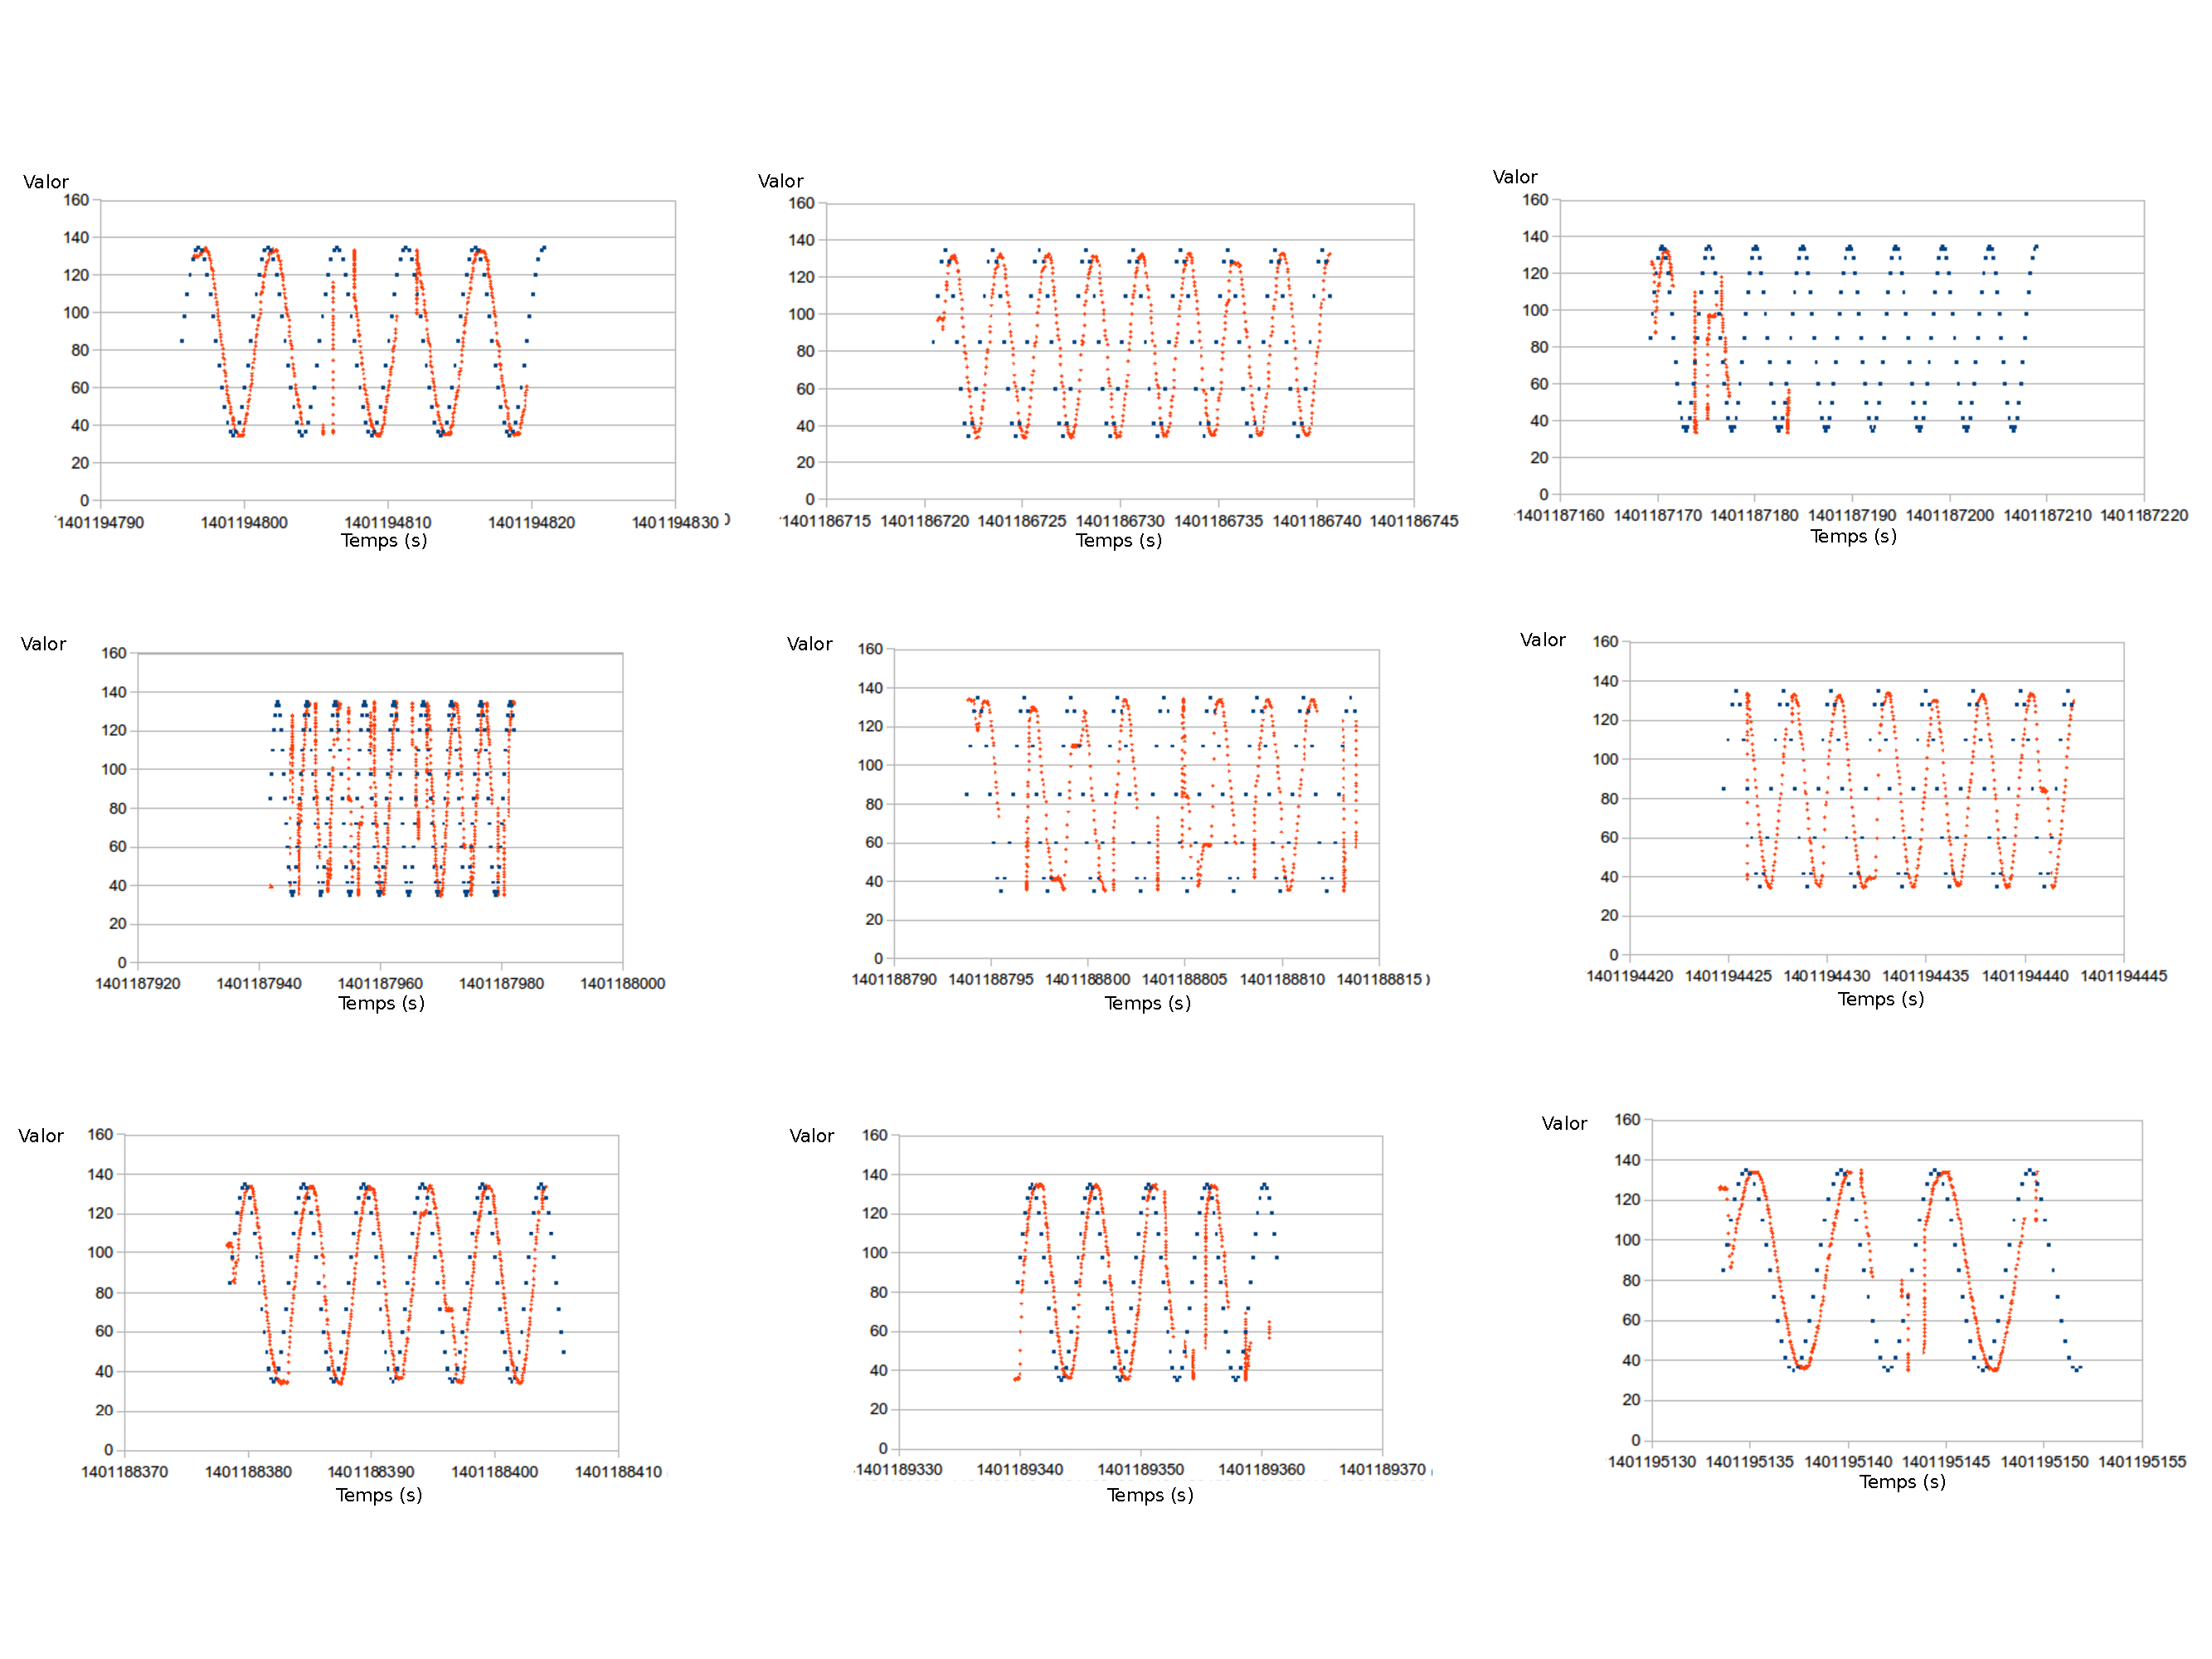
\includegraphics[scale=0.37]{images/sin5H.pdf}
	 \caption{En azul está graficado las posiciones enviadas a 5Hz y en rojo las lecturas. En columnas se encuentran las replicas del mismo método y por filas los tres métodos usados, en orden descendente son liburbi con un cliente, liburbi con dos cliente y python.}
  \label{fig:sin5H}
\end{figure}
\begin{figure}[H]
	\centering
    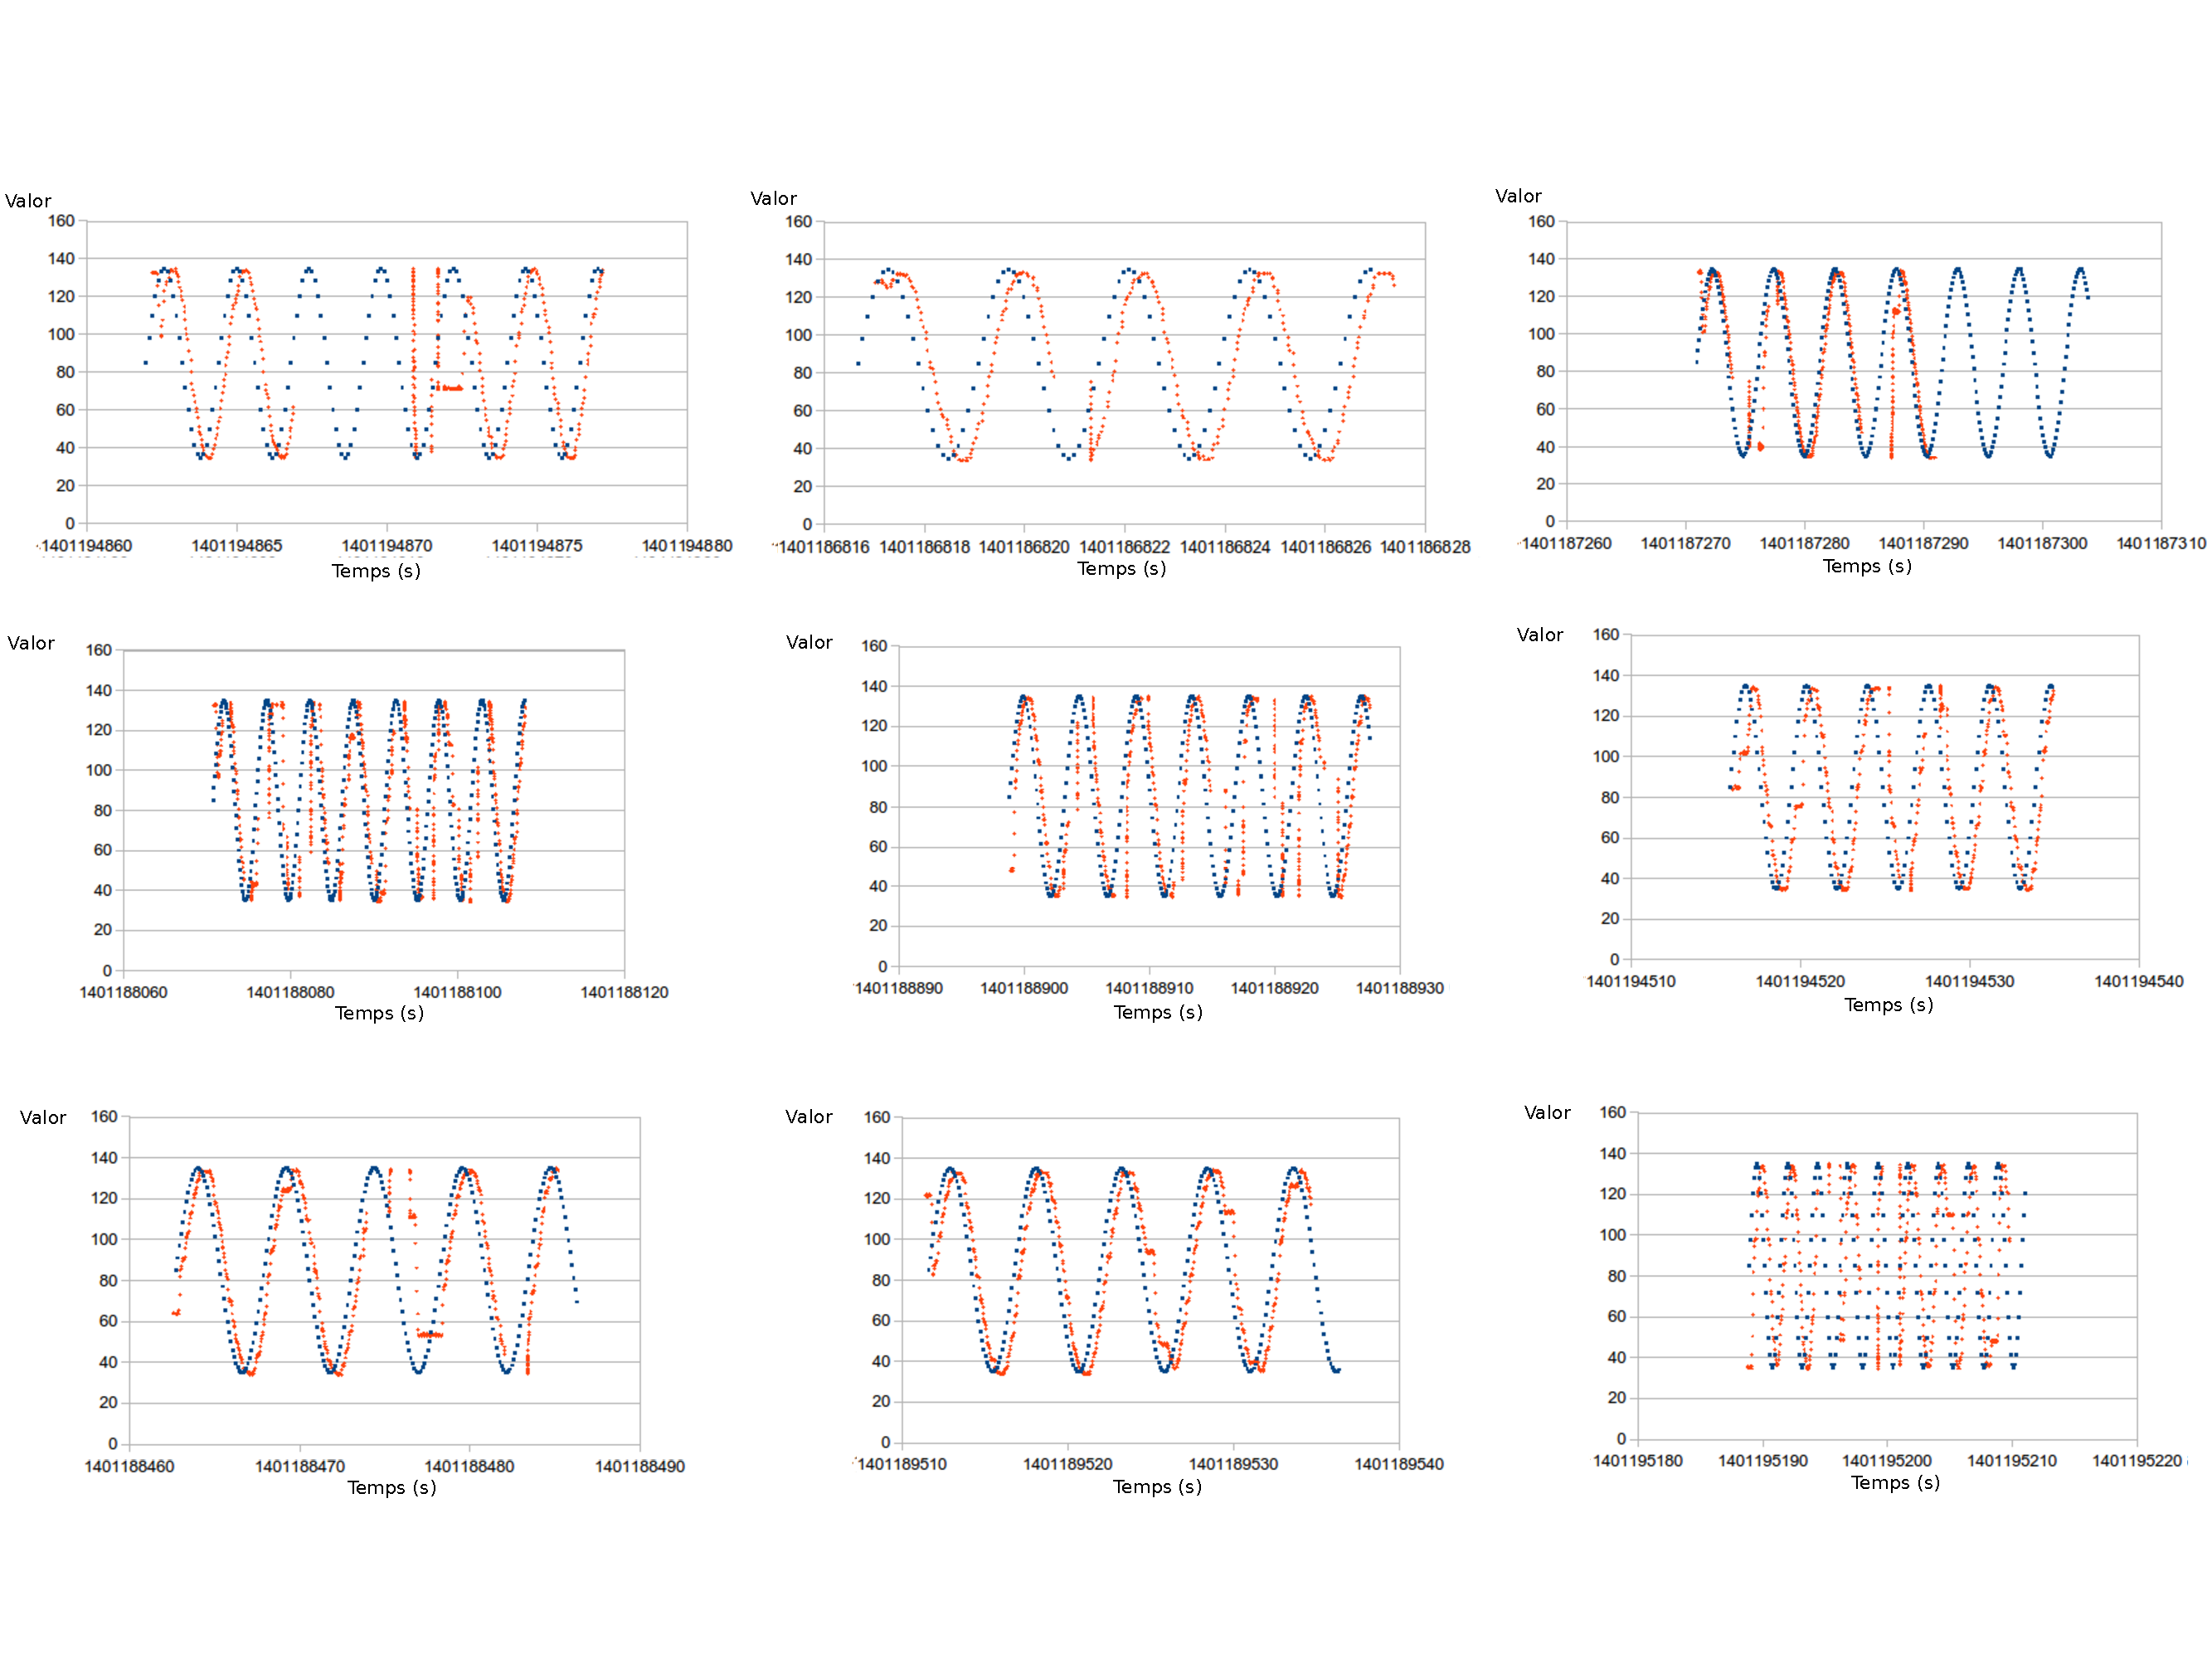
\includegraphics[scale=0.37]{images/sin10H.pdf}
	 \caption{En azul está graficado las posiciones enviadas a 10Hz y en rojo las lecturas. En columnas se encuentran las replicas del mismo método y por filas los tres métodos usados, en orden descendente son liburbi con un cliente, liburbi con dos cliente y python.}
  \label{fig:sin10H}
\end{figure}

En los gráficos de las Figuras \ref{fig:sin1H}, \ref{fig:sin2H}, \ref{fig:sin5H} y \ref{fig:sin10H} se pueden distinguir  dos tipos de errores por los cuales no se sigue bien la trayectoria:

\begin{itemize}
\item La articulación no se mueve:Queda reflejado como una recta roja horizontal y el modulo responsable es el de escritura.
\item No se recibe la posición actual: Queda reflejado como un periodo sin datos. en este caso no se puede saber si la articulación se movía o no\footnote{Por inspección visual se ha comprobado que ambos errores son independientes.}.
\end{itemize}
El caso en el que sólo se usa un solo cliente con liburbi tiene grandes bloqueos en la recepción de y muestra un movimiento más brusco e inconstante.
Entre los dos otros no se puede determinar cual de los dos tiene un mejor seguimiento. Con el fin de marcar la diferencia se ha evaluado bajo otro criterio.
Se han hecho las diferencias de entre el tiempo en que se envía la orden de los picos de la sinusoide y el momento en que se recibe que ha llegado a tal posición. Para comprobar si existe una diferencia se realiza una ANOVA sobre los datos de la Figura \ref{fig:retras} y resuelve con un intervalo de confianza del 95\% y un p-valor del 0.43  se acepta la hipótesis nula y que por tanto el retraso con C++ no es significativamente mayor. 
 
\begin{figure}[H]
	\centering
\begin{tikzpicture}[baseline]
\pgfplotsset{width=13cm,compat=1.10}
\begin{axis}[
xlabel={$replicas$},
ylabel={$tiempo(s)$},
minor y tick num=1,
legend style={at={(0.5,-0.25)},
anchor=north,legend columns=-1},
]
\addplot[blue, only marks] table {data/retrasoPy.dat};
\addplot[black, only marks] table {data/retrasoC++.dat};
\addplot[blue,sharp plot,update limits=false]
coordinates {(0,0.511) (20,0.511)}
node[above] at (axis cs:9,0.511) {0.511};
\addplot[black,sharp plot,update limits=false]
coordinates {(0,0.737) (20,0.737)}
node[above] at (axis cs:9,0.737) {0.737};
\legend{python, liburbi}
\end{axis}
\end{tikzpicture}
	 \caption{Retrasos entre la orden enviada y la acción para los métodos liburbi con dos clientes y python.}
  \label{fig:retras}
\end{figure}

\subsection{Elección del método}
A partir de los resultados anteriores se procede a elegir el caso que garantizará un mejor funcionamiento del paquete a implementar. En la Tabla \ref{comp} se encuentran resumidos los criterios de evaluación.


\begin{table}[H]
\begin{center}
\begin{tabulary}{\textwidth}{|p{4cm}|p{3cm}|p{3cm}|p{3cm}|}
\hline

&\textbf{Python con telnet} & \textbf{C++ con liburbi y 1 cliente} & \textbf{C++ con liburbi y 2 clientes} \\ \hline
Frecuencia máxima de lectura & menor & Mayor & Mayor \\ \hline
Frecuencia media de lectura & Menor& Mayor & Mayor  \\ \hline
Congelaciones en la lectura & Si & Si &Si \\ \hline
Frecuencia de envío& = & = & = \\ \hline
Seguimiento de trayectorias & Bueno & Malo & Bueno \\ \hline
Efecto negativo del envío en la lectura& No & Si & No \\ \hline
Retraso de la respuesta & Menor & Mayor & \\ \hline
Bloqueos de en el envío & Si & Si & Si \\ \hline
\end{tabulary}
\end{center}
\caption{Comparación de los métodos usados y sus resultados en los experimentos.\label{comp}}
\end{table}

En cuanto a recepción de datos se refiere es mas rápido el usando liburbi aunque sufra las mismas congelaciones que usando python y a efectos prácticos para la implementación del paquete es lo mismo que transmita a 10KHz que a 20KHz. Y respecto al envió el seguimiento de la trayectoria és parecido en ambos metodos, python y liburbi con dos clientes, pero parece que tenga un retraso superior el segundo. De todos modos no se considera concluyente el experimento echo pues dada la variabilidad de los resultados es posible que se haya trabajado con pocos datos el análisis sobre el retraso. Finalmente se elige usar la librería liburbi dado que se cree más convincente la ventaja en la adquisición de los datos que el retraso en la respuesta. Por otra parte se ha tenido en consideración que el paquete será más complejo que los experimentos y puede ser útil que la velocidad de ejecución de un programa enn C++ sea mayor que en python.

\newpage
\section{Implementación del paquete de ROS}
\subsection{ROS}
\label{ros}
ROS es el acrónimo de Robot Operating System que lejos de ser un sistema operativo es más bien un marco de trabajo que proporciona unas herramientas y librerías para ayudar a desarrollar software para aplicaciones en robótica. Proporciona entre otros abstracciones de hardware, controladores para dispositivos, herramientas de visualización, comunicación por mensajes, administración de paquetes y todo bajo licencia de software libre.
La principal característica sobre la que se basa ROS es el sistema de comunicación que proporciona. A bajo nivel está basada en el paso de mensajes que pueden ser leídos por diversos procesos simultaneamente. Dichos mensajes se escriben sobre unos canales de comunicación llamados \textit{tópicos} a los que se puede acceder mediante métodos de publicación y suscripción. Sobre los tópicos se puede publicar o se puede suscribir desde un terminal o bien cualquier objeto de ROS a los que se les llama \textit{nodos}. Todos los nodos que se pretendan tener comunicados entre si deben estar creados sobre el mismo núcleo o \textit{roscore}.


Todos los programas que se pretendan ejecutar sobre ROS son creados dentro de un paquete i todo paquete de ROS contiene una serie de archivos necesarios para su compilación:
\begin{itemize}
\item manifest.xml: Se incluye información sobre el nombre del paquete, el autor, tipo de licencia y paquetes externos necesarios.
\item CMakelists.txt: Se indica el uso de librerías, el uso de mensajes propios del paquete y se declaran los ejecutables.
\item mainpage.dox: Permite hacer un resumen explicativo del paquete.
\item archivos ejecutables: ROS permite usar su API con C++ i python.
\item carpeta msg: Contiene los archivos *.msg donde se definen los mensajes propios del paquete.
\item carpeta srv: contiene los archivos *.srv donde se definen los servicios propios del paquete.
\item Carpeta launch: Contiene los archivos *.launch que permiten lanzar varios nodos de diferentes paquetes y tipos con los parámetros convenientes.

\end{itemize}
\subsection{Paquet aibo{\_}server }
Se pretende implementar una paquete que en lanzarse se conecte al AIBO indicado por la dirección IP. Una vez conectado debe recoger los datos enviados por el servidor URBI del AIBO y publicarlos sobre una serie de tópicos. De forma inversa debe tratar los valores de las articulaciones publicados en un tópico al que esta suscrito y enviarlos al servidor con el fin de actuar sobre la plataforma.

\begin{figure}[H]
	\centering
    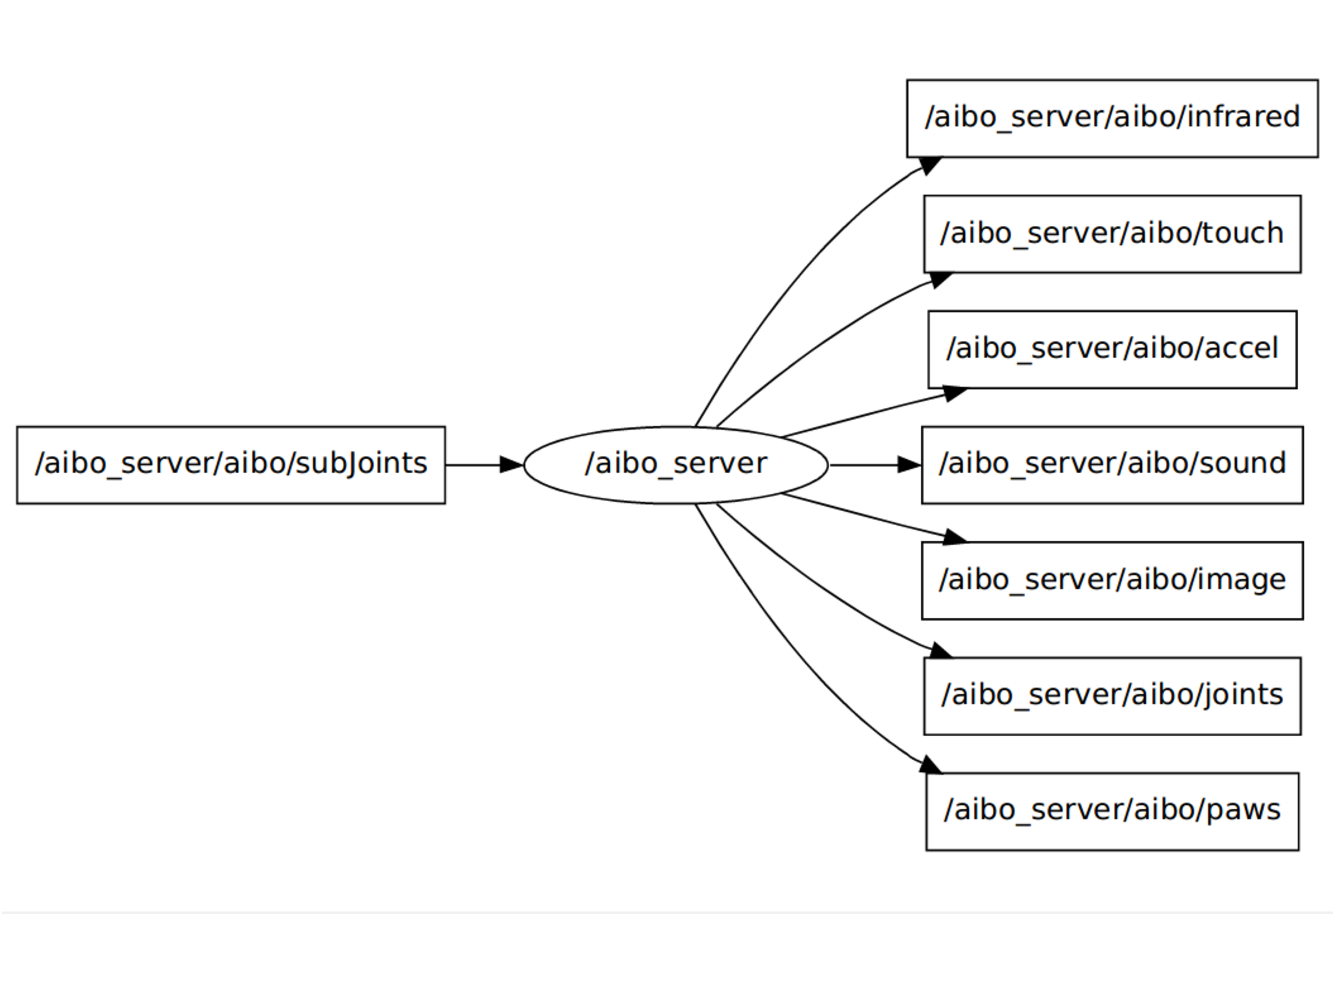
\includegraphics[scale=0.7]{images/aiboserverNodo.pdf}
	 \caption{Nodo aibo{\_}server.}
  \label{fig:aiboserv}
\end{figure}

Para la realización de este paquete de ROS se han tenido en cuenta las siguientes consideraciones:
\begin{itemize}
\item Incluir en el manifest.xml los paquetes de ROS necesarios para su implementación:
\begin{itemize}
\item roscpp: permite utilizar la API ROS para C++.
\item std{\_}msgs: permite el uso de unos mensajes estándar.
\item sensor{\_}msgs: permite el uso de mensajes especialmente destinados a ciertos tipos de sensores.
\end{itemize}
\item Implementación de los archivos necesarios para el ejecutable:
\begin{itemize}
\item AiboNode.cpp: Archivo a partir del que se crea el ejecutable del paquete. En el se encuentra toda la estructura del programa.
\item AiboServer.cpp y AiboServer.h: Se define la clase aibo en la que se basa AiboNode.cpp.
\item AiboParams.h: se definen las constantes.
\end{itemize} 
\item Definición de los mensajes propios:
\begin{itemize}
\item Accel.msg: Mensaje destinado al acelerómetro.
\item Bumper.msg y BumperArray.msg: Mensaje destinado a los sensores de contacto de las patas.
\item IRArray.msg: Mensaje destinado a los tres infrarojos.
\item Jointes.msg: Mensaje destinado a las articulaciones.
\item Sound.msg: Mensaje destinado al envío de sonido.
\item TouchArray.msg: mensaje destinado a los sensores de tacto de la espalda y la cabeza.
\end{itemize}
\item Modificación del CMakeList.txt para incluir los mensajes y los archivos C++ descritos además de la librería liburbi.
\end{itemize}

\subsubsection{Estructura del programa}
Basándose en los resultados de la sección anterior, Sección \ref{seccomp}, se ha procedido a la implementación del paquete de ros usando liburbi i dos clientes, uno para la recepción  y otro para el envío.

La estructura del programa que se ha implementado se puede ver en la Figura \ref{fig:aiboserver}.
\begin{figure}[H]
	\centering
    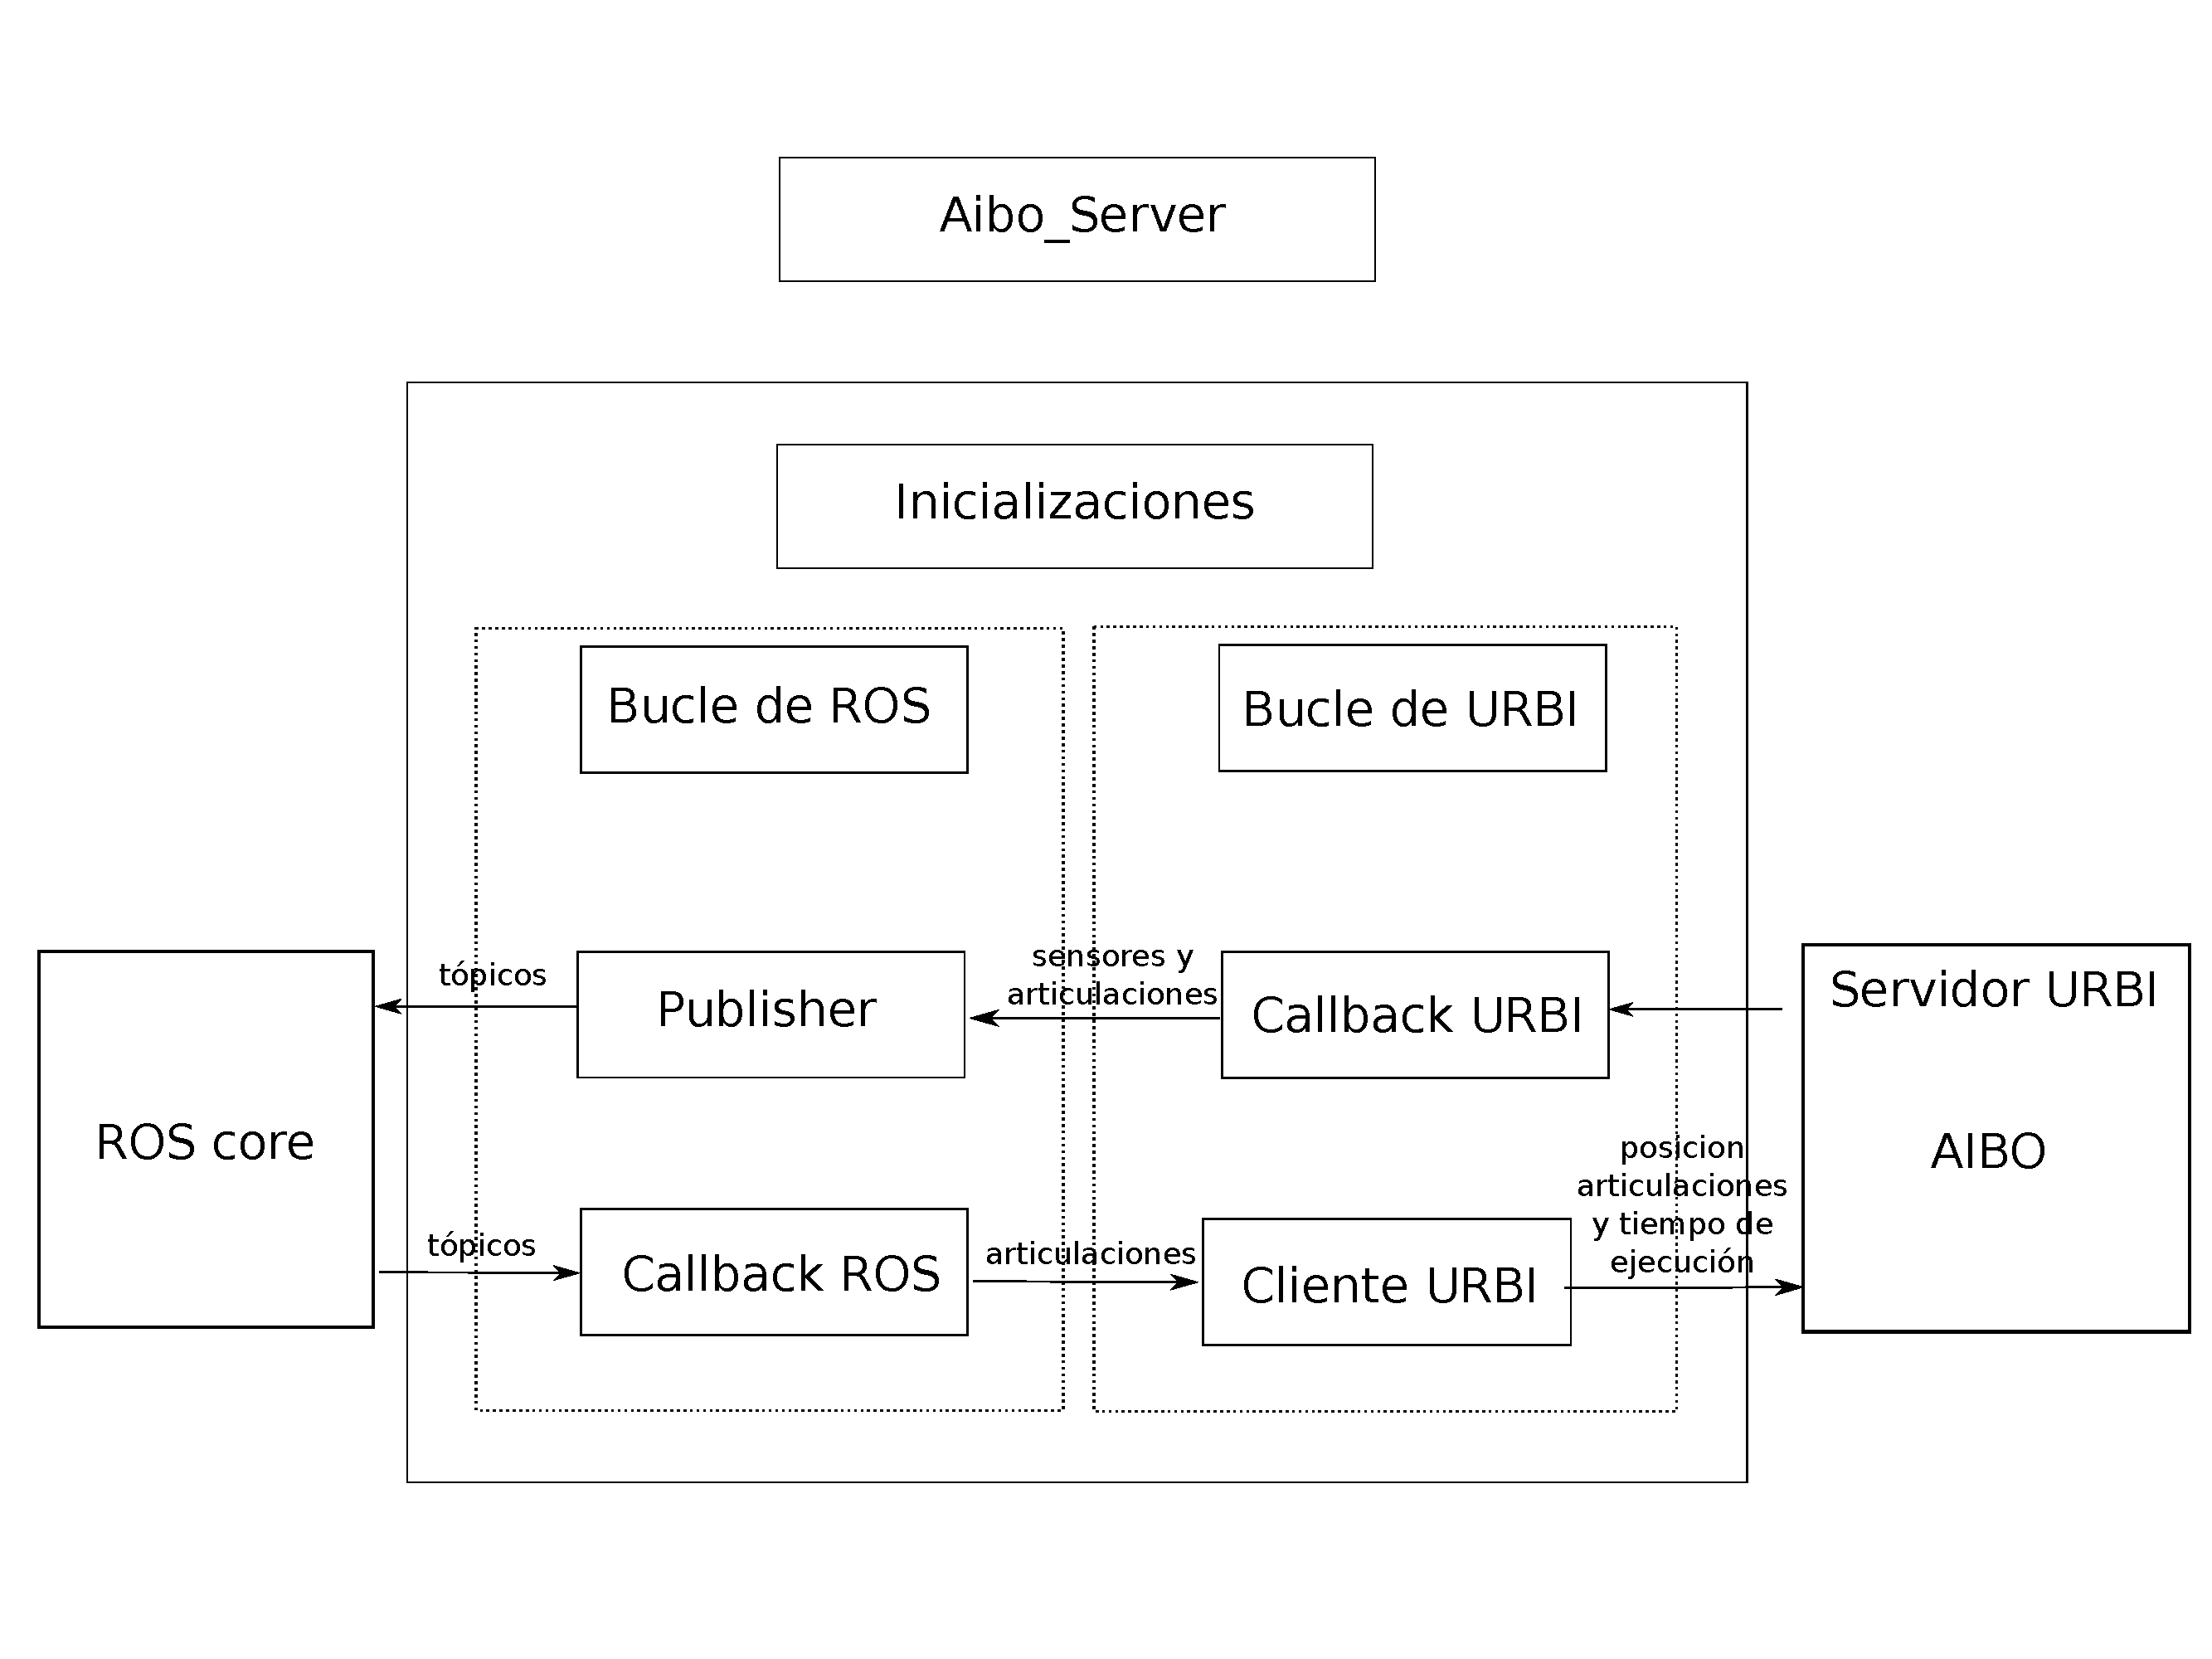
\includegraphics[scale=0.35]{images/Aibo_Server.pdf}
	 \caption{Estructura básica del ejecutable aibo{\_}server.}
  \label{fig:aiboserver}
\end{figure}

\begin{itemize}
\item Inicializaciones: 
\begin{itemize}
\item Inicialización del nodo de ROS:
\begin{itemize}
\item Creación del nodo: Se le otorga un identificador al nodo, en este caso aibo{\_}server.
\item Definición de la frecuencia de ejecución del bucle de ROS.
\item Se inicializa el \textit{Subscriber} que permitirá llamar llamara al Callback de ROS.   
\end{itemize}

\item Inicialización de la instancia de la clase \textbf{aibo}:
\begin{itemize}
\item Inicialización de los clientes URBI de lectura y escritura.
\item Creación de los tópicos e inicialización de los \textit{Publishers} que publicaran en ellos.
\item Definición del Callback de URBI para cada sensor y articulación.
\item Demanda del envio de datos desde URBI.
\item Definición del método de tratamiento de ordenes que usará el servidor URBI.
\end{itemize}
\end{itemize}
\item Bucle de URBI:
\begin{itemize}
\item Se crea un hilo de ejecución en paralelo donde se lleva acabo el bucle de URBI.
\item Llamada a los callbacks de URBI: En los callbacks se guardan los valores obtenidos en las variables de clase correspondientes.

\end{itemize}
\item Bucle de ROS:
\begin{itemize}
\item Publicación de las variables de los sensores y articulaciones en los tópicos correspondientes.
\item Llamada al callback de ROS: Éste envía la orden al servidor URBI mediante el cliente de envío.
\end{itemize}
\end{itemize}
\subsubsection{Resultados}

Por lo que respecta la adquisición de los valores de sensores y articulaciones se ha conseguido obtenerlos todos ellos trabajando a una frecuencia de 10Hz. Con tal de comprobar que el refresco de los tópicos es correcto se ha accedido a mostrar por el terminal todos los tópicos mostrando su frecuencia de refresco Figura \ref{fig:getT} y por otro lado, al mismo tiempo, se ha graficado el valor de un sensor en la Figura \ref{fig:addacc} El echo de que el gráfico muestre un cierto ruido indica que el valor se esta refrescando correctamente, por lo contrario si el valor de la gráfica es constante indica que no se está refrescando correctamente.

\begin{figure}[H]
	\centering
    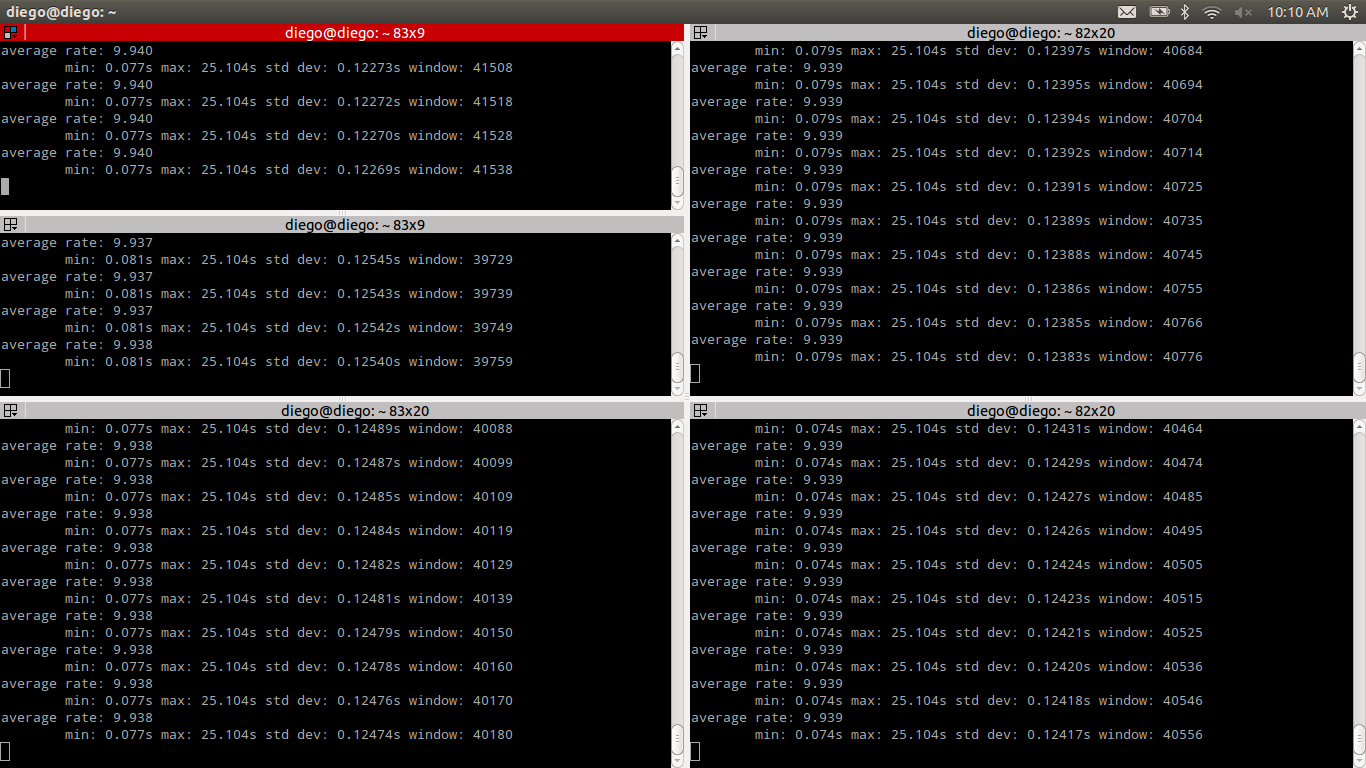
\includegraphics[scale=0.3]{images/getTopics.png}
	 \caption{Consulta de la frecuencia de publicación en los diferentes tópicos de aibo{\_}server.}
  \label{fig:getT}
\end{figure}

\begin{figure}[H]
	\centering
    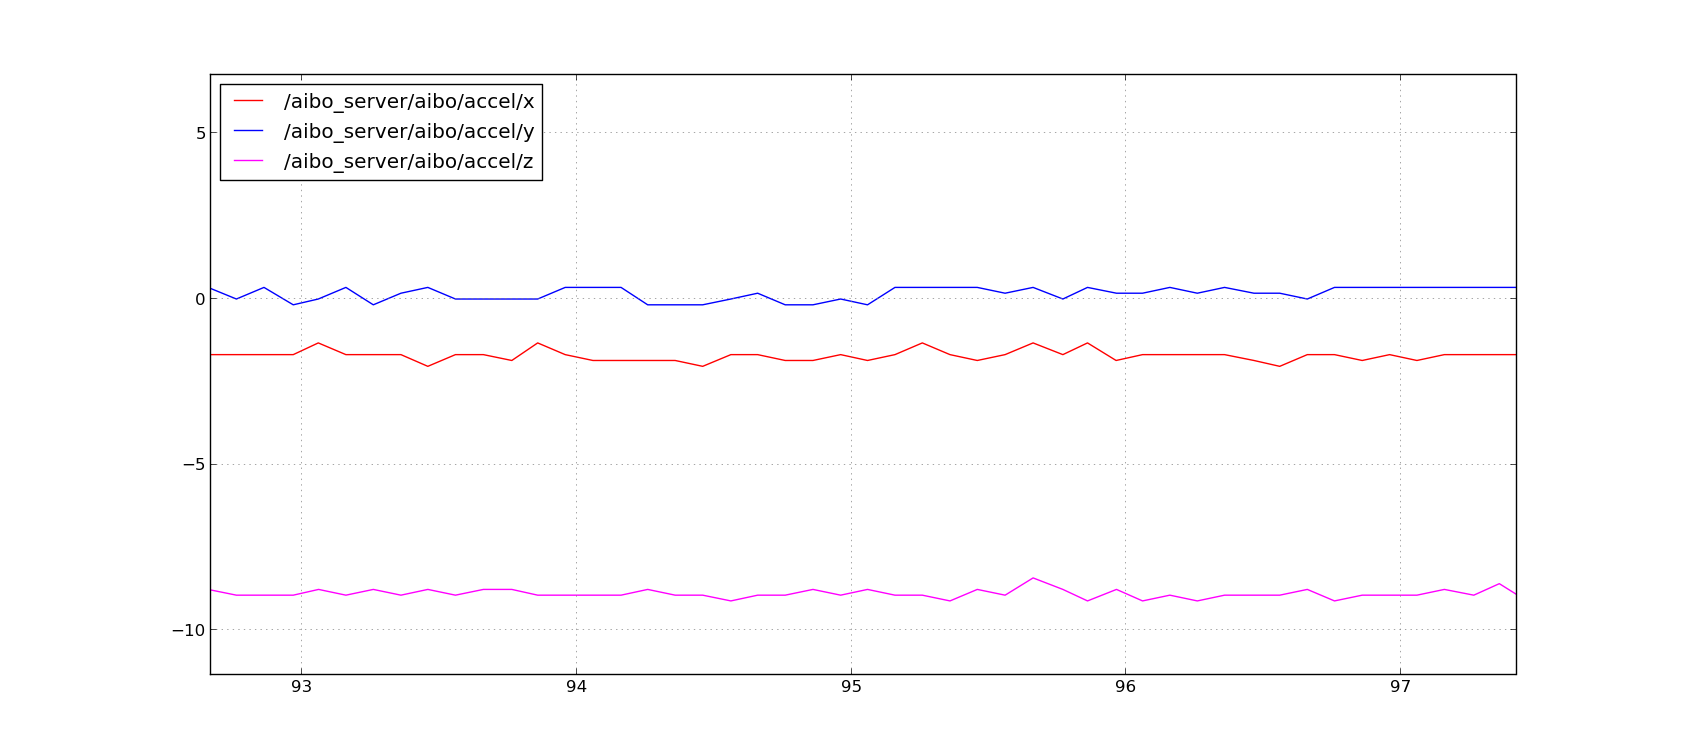
\includegraphics[scale=0.4]{images/addaccel.png}
	 \caption{Valores de los acelerometros graficados usando la herramienta rqt{\_}plot.}
  \label{fig:addacc}
\end{figure}

Con tal de valorar el envío de las posiciones se procede a realizar un paquete de ROS que permita cuantificar los resultados.

El primer test realizado es el mismo que con el que se ha valorado las experimentaciones de la sección \ref{seccomp}. Se trata de aplicar una sinusoide al movimiento de una articulación.

Para la realización del test se ha implementado un sencillo programa\footnote{El código se puede encontrar en el Anexo \ref{sinlegROS}} que crea un nodo que publica sobre el tópico \textit{/aibo{\_}server/aibo/subjoints/jointRF1} valores que varían de forma sinusoidal. 
La estructura entre los nodos se muestra en la figura \ref{fig:ASSL}.
\begin{figure}[H]
	\centering
    
\includegraphics[scale=0.35]{images/rosgraphASsin.pdf}
	 \caption{Estructura de ROS con los nodos aibo\_server y SinLeg.}
  \label{fig:ASSL}
\end{figure}

De lo extraído en varias replicas a diversas frecuencias se puede reportar que el seguimiento de de la trayectoria lleva un retraso mínimo entorno a los 0.5 segundos que era el retraso propio obtenido en las experimentaciones de la sección \ref{secenvdades} aunque por lo general como se puede observar en las Figuras \ref{fig:ASsin2Hz}, \ref{fig:ASsin7Hz} y \ref{fig:ASsin10Hz} 
dicho retraso no es la norma general estando el retraso medio muy por encima de éste.
\begin{figure}[H]
	\centering
    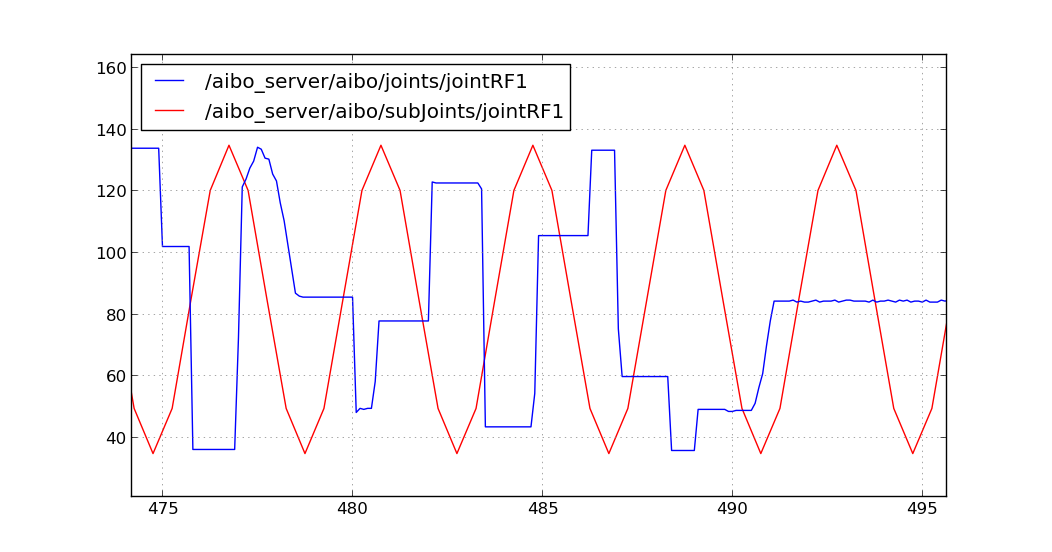
\includegraphics[scale=0.66]{images/sinlegWR/10Ry2S.png}
 	\caption{Entrada y respuesta del sistema ante una señal sinusoidal de enviando puntos a 2Hz.}
  \label{fig:ASsin2Hz}
\end{figure}
\begin{figure}[H]
	\centering
    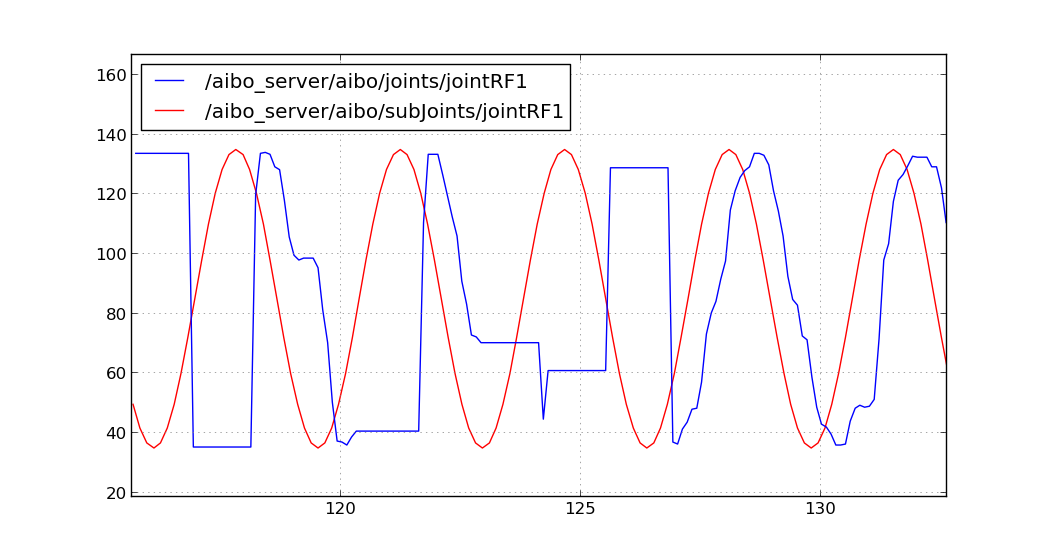
\includegraphics[scale=0.66]{images/sinlegWR/10Ry7S.png}
 	\caption{Entrada y respuesta del sistema ante una señal sinusoidal de enviando puntos a 7Hz.}
  \label{fig:ASsin7Hz}
\end{figure}
   \begin{figure}[H]
	\centering
    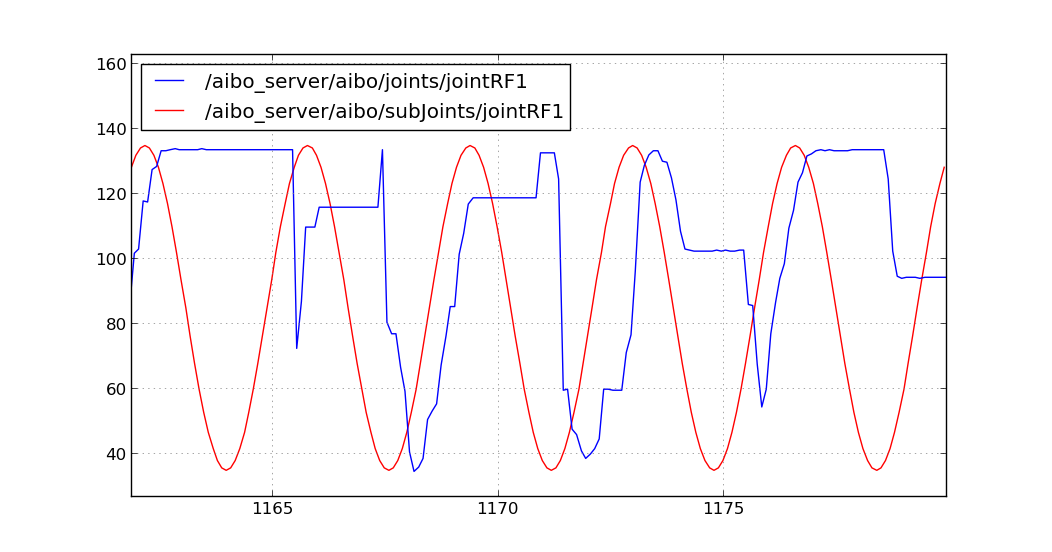
\includegraphics[scale=0.66]{images/sinlegWR/10Ry10SAll.png}
 	\caption{Entrada y respuesta del sistema ante una señal sinusoidal de enviando puntos a 10Hz.}
  \label{fig:ASsin10Hz}
\end{figure}

Además el modulo sufre bloqueos que pueden durar minutos, igual que en las secciones anteriores.
Valorando el modulo se puede concluir que no funciona de la forma deseada ni requerida para varias aplicaciones en las que se requiere una lectura y respuesta rápida del sistema. 

\subsubsection{Mejoras}
Los problemas encontrados, tras un proceso de depuración se pueden clasificar de la siguiente forma:
\begin{itemize}
\item Cortas congelaciones en la recepción de los valores de los sensores y articulaciones: respeto a ello ya se ha probado que en las experimentaciones anteriores que los resultados no podían mejorar usando liburbi.
\item Envío de la orden correctamente pero tarda en realizar el movimiento: Este es un problema interno del tratamiento de las ordenes del servidor URBI y que por lo tanto no se puede hacer nada al respeto des de el punto de vista del cliente.
\item Bloqueo en enviar la orden de movimiento: Como en las experimentaciones de la sección anterior se producen bloqueos debidos a que la función de liburbi que permite enviar ordenes se queda bloqueada. Estos bloqueos hacen que se bloquee todo el nodo durante segundos e incluso minutos.
\end{itemize}

A raíz del ultimo problema comentado se ha implementado una solución que evita dos de las consecuencias que conlleva.
En primer lugar en caso de que se produzca un bloqueo en el envío de una posición del cliente al servidor, éste no debe afectar a la recepción de las demás variables. Como solución se propone que el envió y la recepción se produzcan en dos threads distintos e independientes. 
En segundo lugar se desea evitar los bloqueos en el envío. Esto se pretende hacer inicializando un tercer cliente URBI de manera que cuando el cliente de envío se quede bloquee en alguna orden el nuevo cliente lo reemplazara en el envío mientras éste se reinicializa. i en caso de bloqueo del nuevo cliente se espera que el primero, ya reinicializado tome el relevo.
Bajo estas ideas se ha reescrito el callback de ROS como muestra el diagrama de la figura \ref{fig:Call}.

\begin{figure}[H]
	\centering
    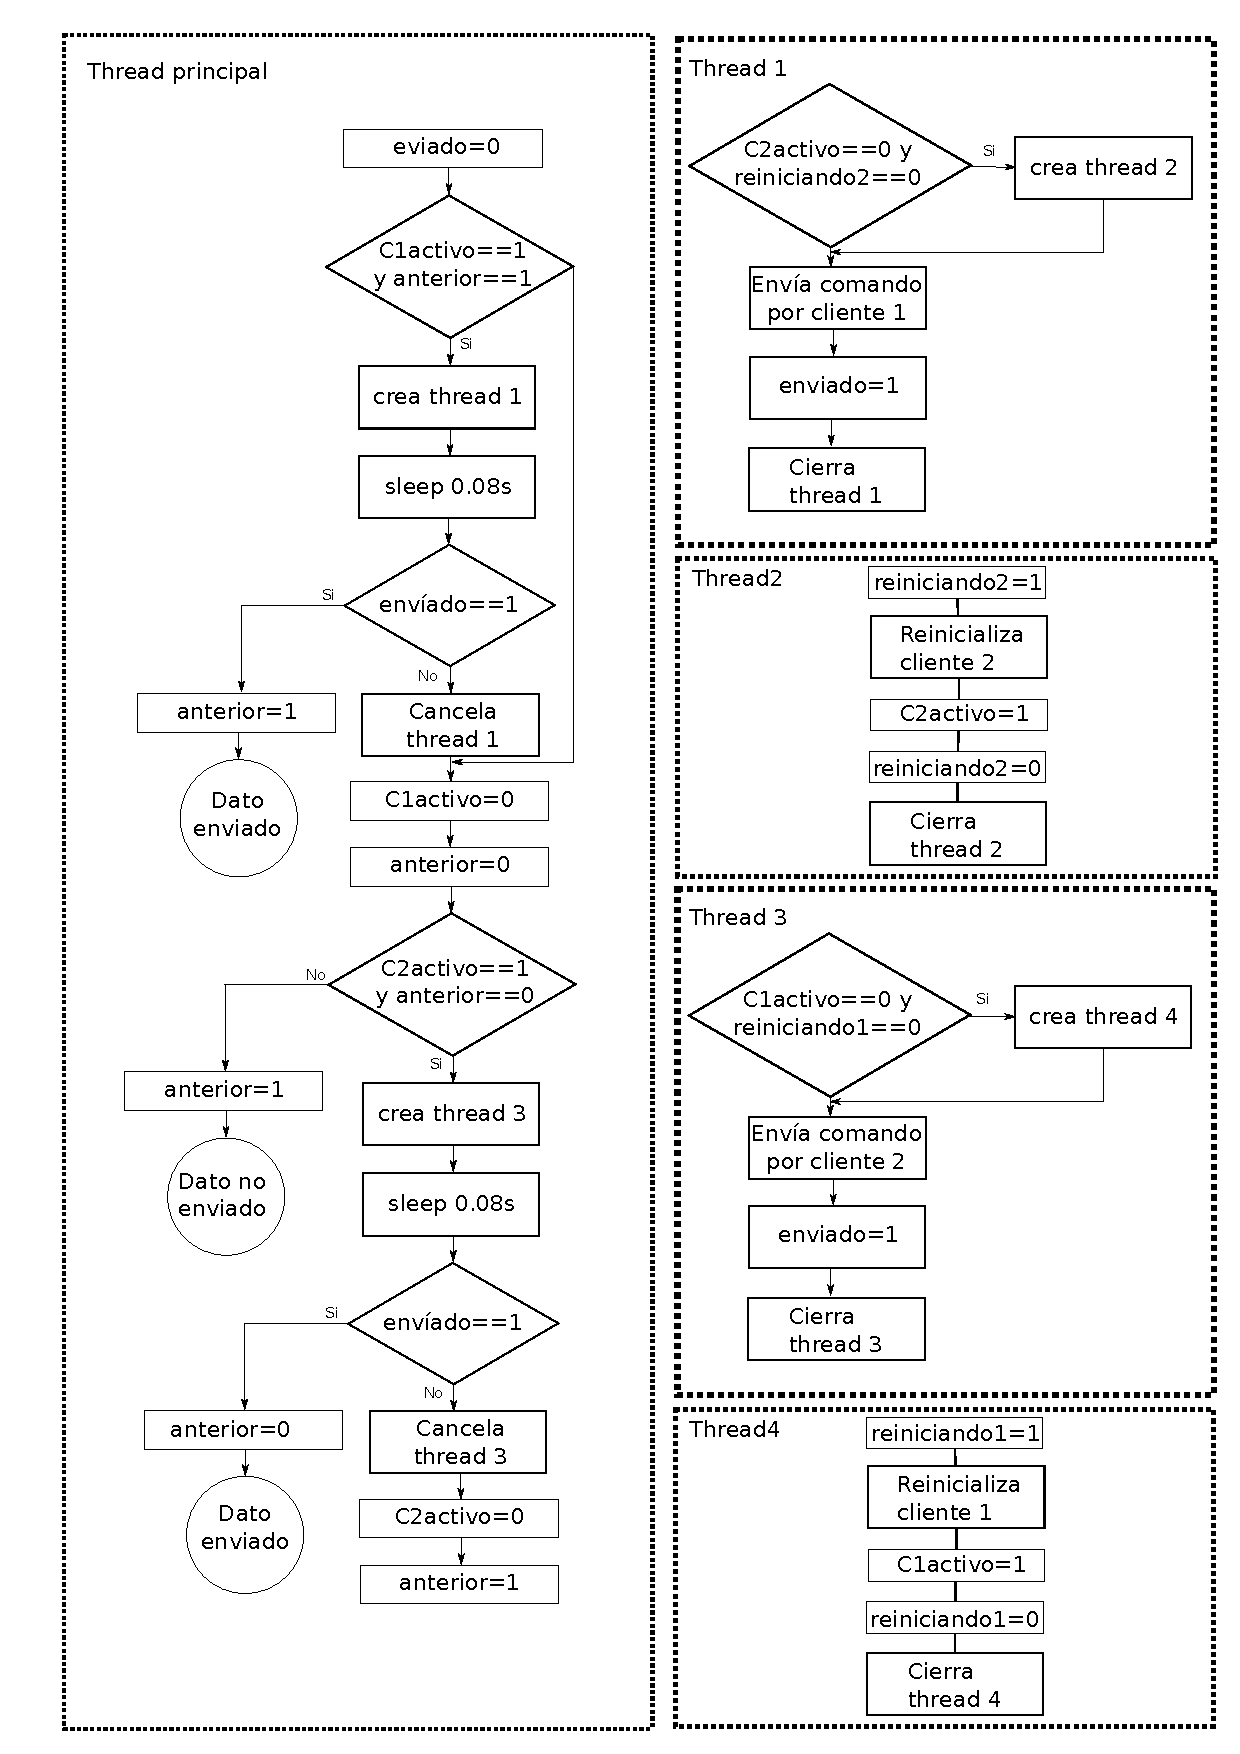
\includegraphics[scale=0.77]{images/esquemaCall.pdf}
	 \caption{Diagrama del callback de ROS. Los flags \textit{anterior}, \textit{C1activo} y \textit{C2activo}  se inicializan con valor 1 y los flags \textit{reiniciando1} y \textit{reiniciando2} se inicializan a 0.}
  \label{fig:Call}
\end{figure}

Con esta modificación se ha conseguido que el envío de datos, que de forma natural con liburbi es de forma síncrona, puesto que la función de envío espera una respuesta del servidor, se trate de forma asíncrona. Este modo no garantiza la llegada de todos los paquetes de datos pero gana en velocidad de transmisión y evita los bloqueos.

Volviendo de nuevo a comprobar los resultados tras la modificación se vuelve a aplicar un movimiento sinusoidal al movimiento de una articulación.

En la Figura \ref{fig:ASempiezamala} se ve como tras un primer seguimiento de la trayectoria aceptable empieza una zona donde el seguimiento es mucho peor. Esta zona que continua en la Figura \ref{fig:ASpeor} Es un periodo de tiempo en que la comunicación con el AIBO es realmente mala y donde surgían los bloqueos. Tras implementar el nuevo callback el callback la comunicación no se corta, dado que se turnan los dos clientes de envío, pero no sigue bien la trayectoria pues los bloqueos son sucesivos.

\begin{figure}[H]
	\centering
    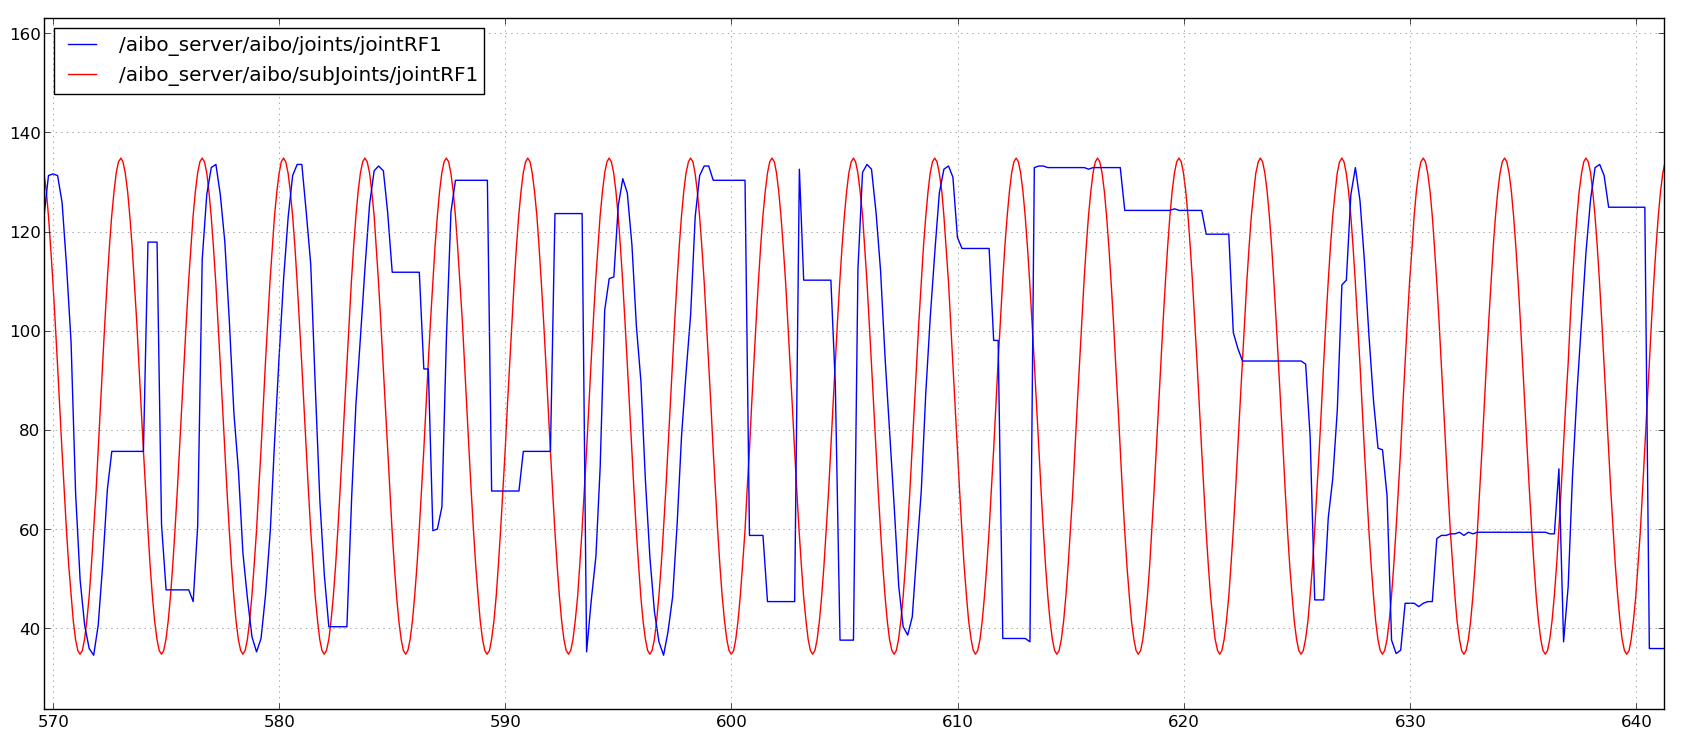
\includegraphics[scale=0.375]{images/sinlegWR/mejorado/empiezamala.png}
 	\caption{Entrada, en rojo, y respuesta, en azul, del sistema ante una señal sinusoidal de enviando puntos a 5Hz. Empiezan a producirse bloqueos.}
  \label{fig:ASempiezamala}
\end{figure}
\begin{figure}[H]
	\centering
    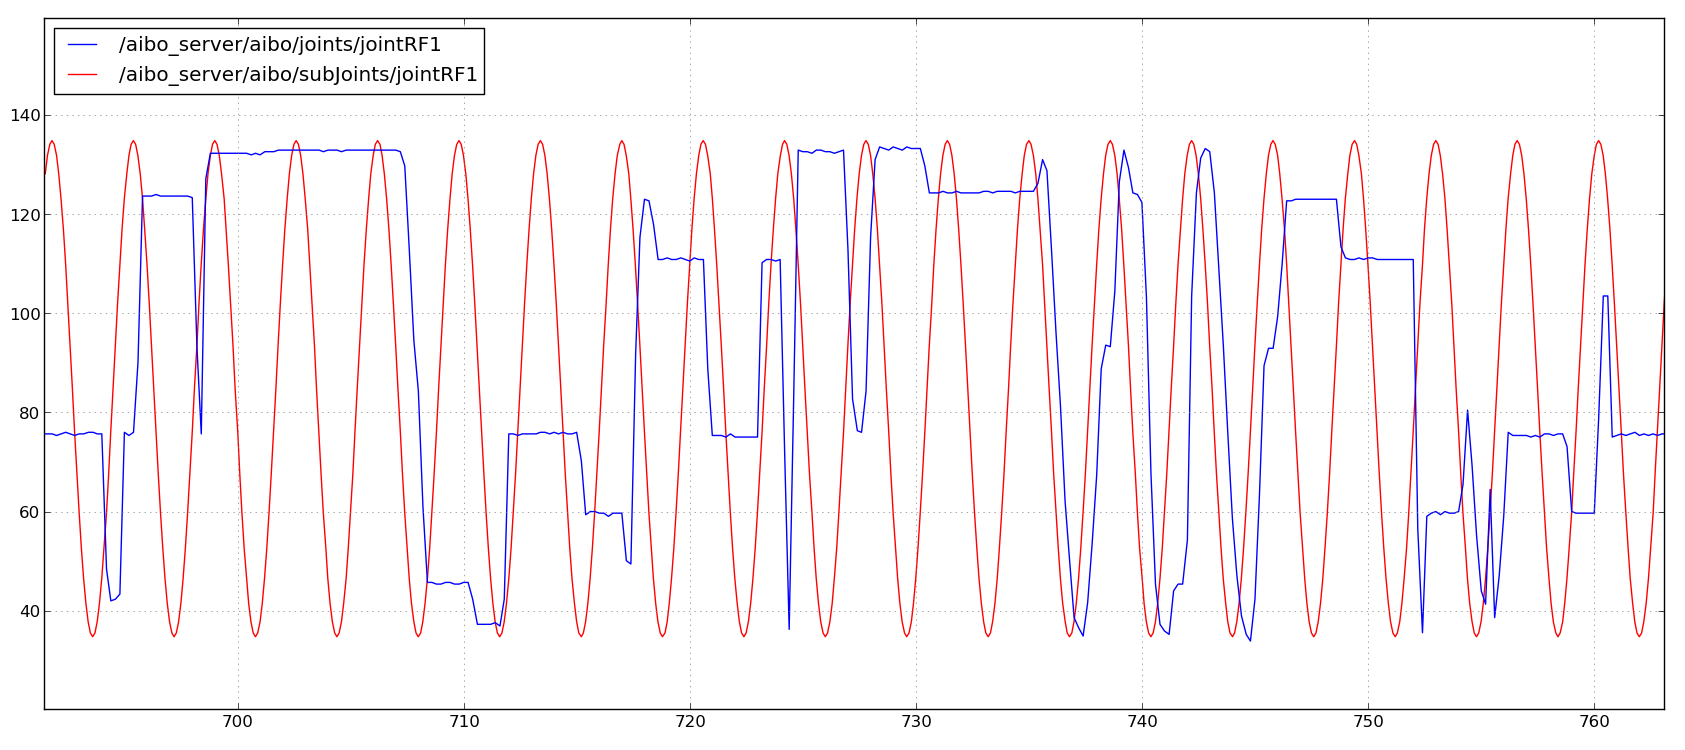
\includegraphics[scale=0.375]{images/sinlegWR/mejorado/peora5hz.png}
 	\caption{Entrada, en rojo, y respuesta, en azul del sistema ante una señal sinusoidal de enviando puntos a 5Hz. Se producen bloqueos que se intentan evitar.}
  \label{fig:ASpeor}
\end{figure}

En la Figura \ref{fig:ASrecupera} se ve como llega un punto, tras una serie de sucesivos bloqueos de ambos clientes, se vuelve a recuperar un buen seguimiento de la trayectoria.
 
\begin{figure}[H]
	\centering
    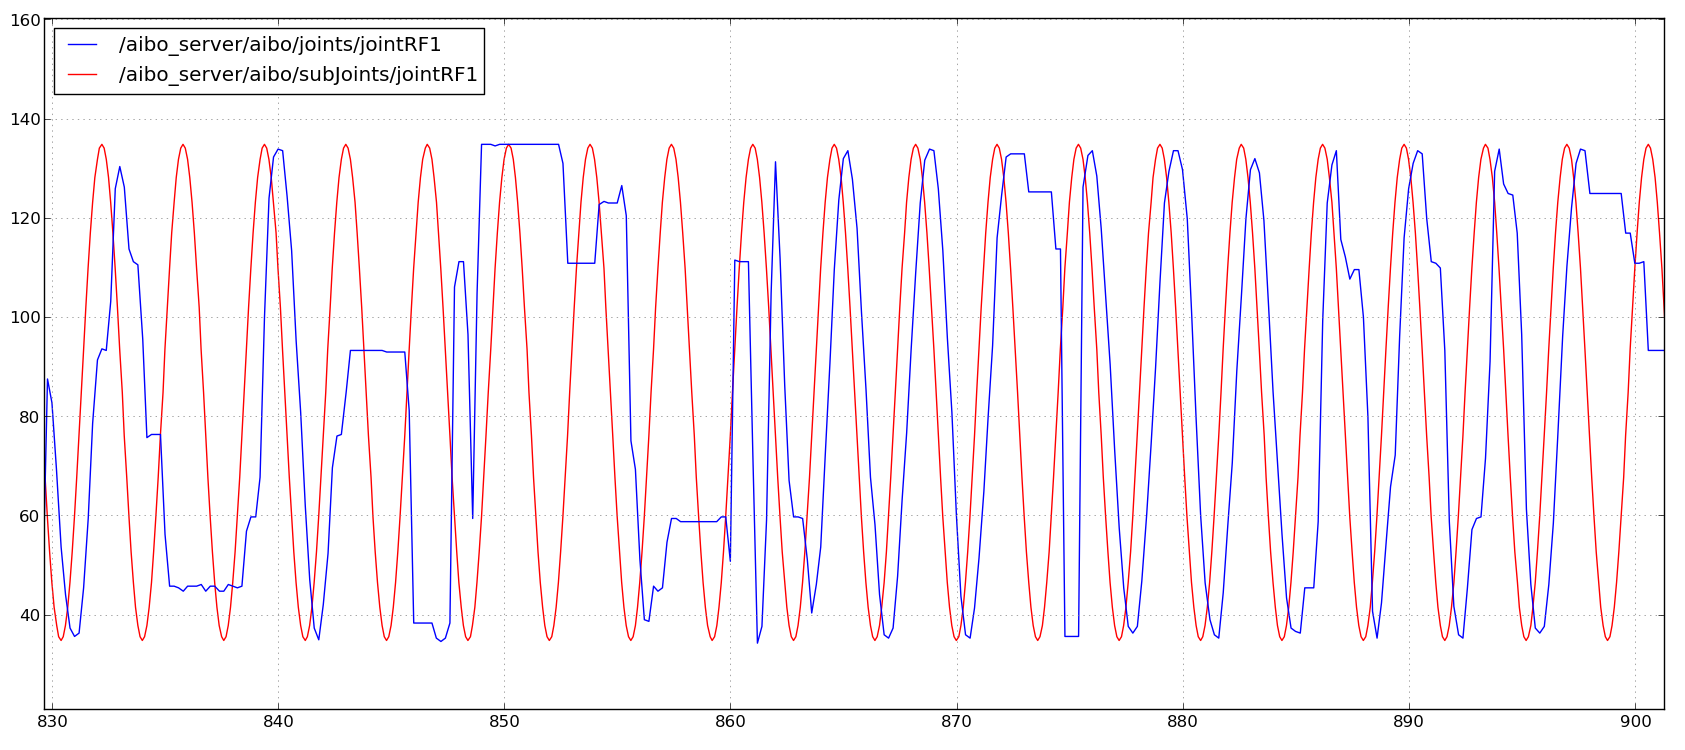
\includegraphics[scale=0.375]{images/sinlegWR/mejorado/recupera.png}
 	\caption{Entrada, en rojo, y respuesta, en azul, del sistema ante una señal sinusoidal de enviando puntos a 5Hz. Recuperación del seguimiento de la trayectoria.}
  \label{fig:ASrecupera}
\end{figure}

Finalmente en la Figura \ref{fig:ASbuena} se puede observar como en algunos momentos el seguimiento de la trayectoria es satisfactorio. Cabe recordar que en estos gráficos obtenidos mediante la herramienta de ROS rqt{\_}plot no se pueden diferenciar si el gráfico no muestra un buen seguimiento debido a la recepción de datos o a que realmente no se está siguiendo bien la trayectoria. Basándose en los resultados de la Sección \ref{compenvio} se puede decir que los bloqueos máximos debidos la recepción son excepcionalmente de más de 2 segundos y por lo tanto menospreciables frente los bloqueos que se muestran en los gráficos.
 \begin{figure}[H]
	\centering
    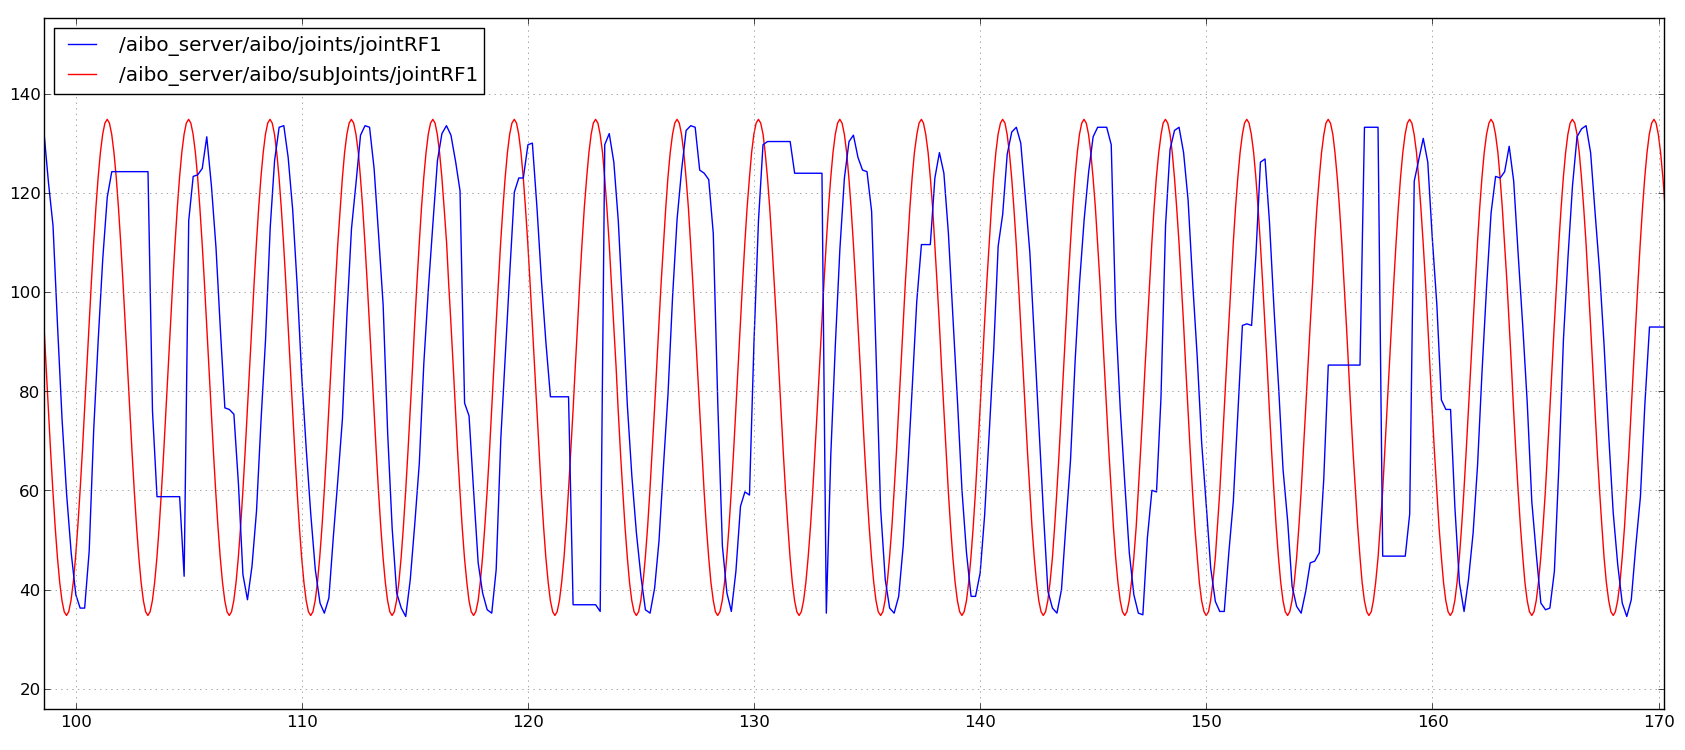
\includegraphics[scale=0.38]{images/sinlegWR/mejorado/mejor5Hz.png}
 	\caption{Entrada,en rojo, y respuesta, en azul, del sistema ante una señal sinusoidal de enviando puntos a 5Hz. Buen seguimiento de la trayectoria.}
  \label{fig:ASbuena}
\end{figure}


\subsubsection{Demostración}
Con tal de asegurar el funcionamiento del paquete aibo{\_}server se ha realizado un programa demuestra como se pueden sincronizar dos o varios AIBO compartiendo variables de estado los unos con los otros. 
En esta demostración en particular se pretende que un AIBO imite los movimientos que realice otro. Es uno de las aplicaciones en que el flujo de datos es realmente grande, dado que las posiciones se modificaran dato a dato, y pondrá realmente a prueba la capacidad del modulo implementado.
Se ha creado un paquete el que incluye un programa\footnote{El código se puede encontrar en el Anexo \ref{mimiccode}.} con un nodo que esta suscrito a el tópico de lectura de las articulaciones de un nodo aibo{\_}server y los publica sobre el tópico de escritura de otro nodo aibo{\_}server. Para crear estos tres nodos se ha hecho un archivo .launch que crea dos nodos del tipo aibo{\_}server con los nombres \texttt{/ai1} y \texttt{/ai2} y un tercer nodo como el descrito. La estructura resultante es la de la Figura \ref{fig:mimic}.


\begin{figure}[H]
	\centering
    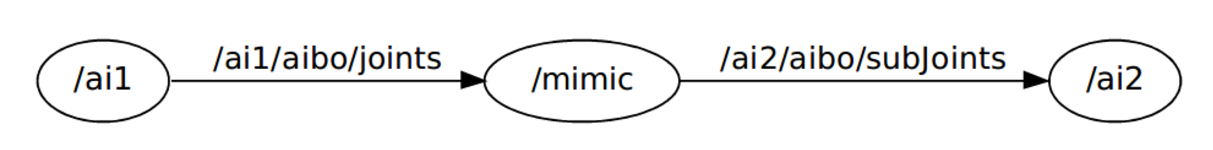
\includegraphics[scale=0.75]{images/mimic.pdf}
	 \caption{Estructura de los nodos de ROS en la demostración de sincronización.}
  \label{fig:mimic}
\end{figure}

En las Figuras \ref{fig:resumimic} y \ref{fig:resumimic2} se puede observar como reacciona las una articulación de ambos AIBOs al mover manualmente uno de ellos. 
%MASGRAFICOs
\begin{figure}[H]
	\centering
    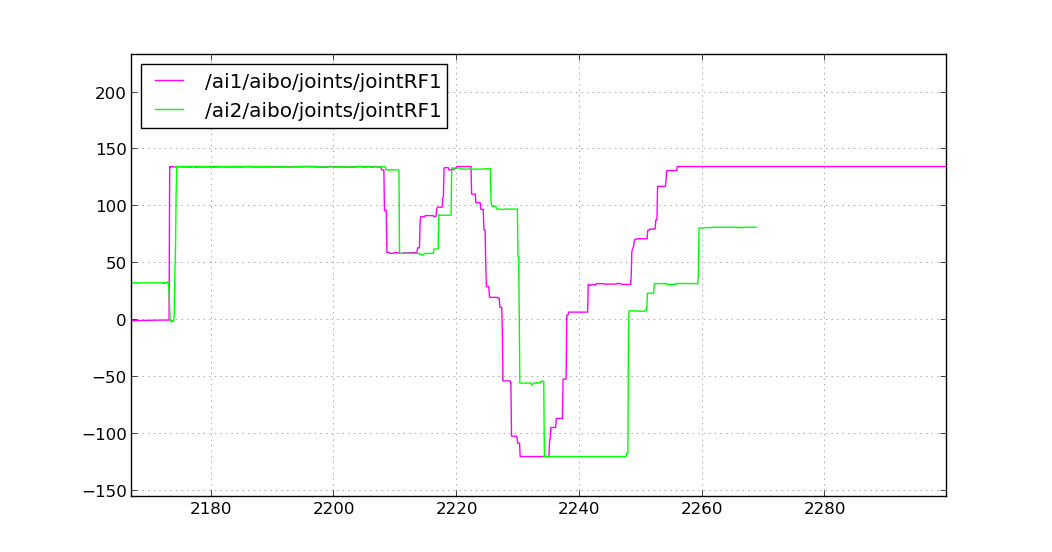
\includegraphics[scale=0.655]{images/mimic/retmin2.png}
	 \caption{Posición de la articulación del AIBO movido manualmente, en fucsia, y del AIBO que hace la imitación, en verde.}
  \label{fig:resumimic}
\end{figure}
\begin{figure}[H]
	\centering
    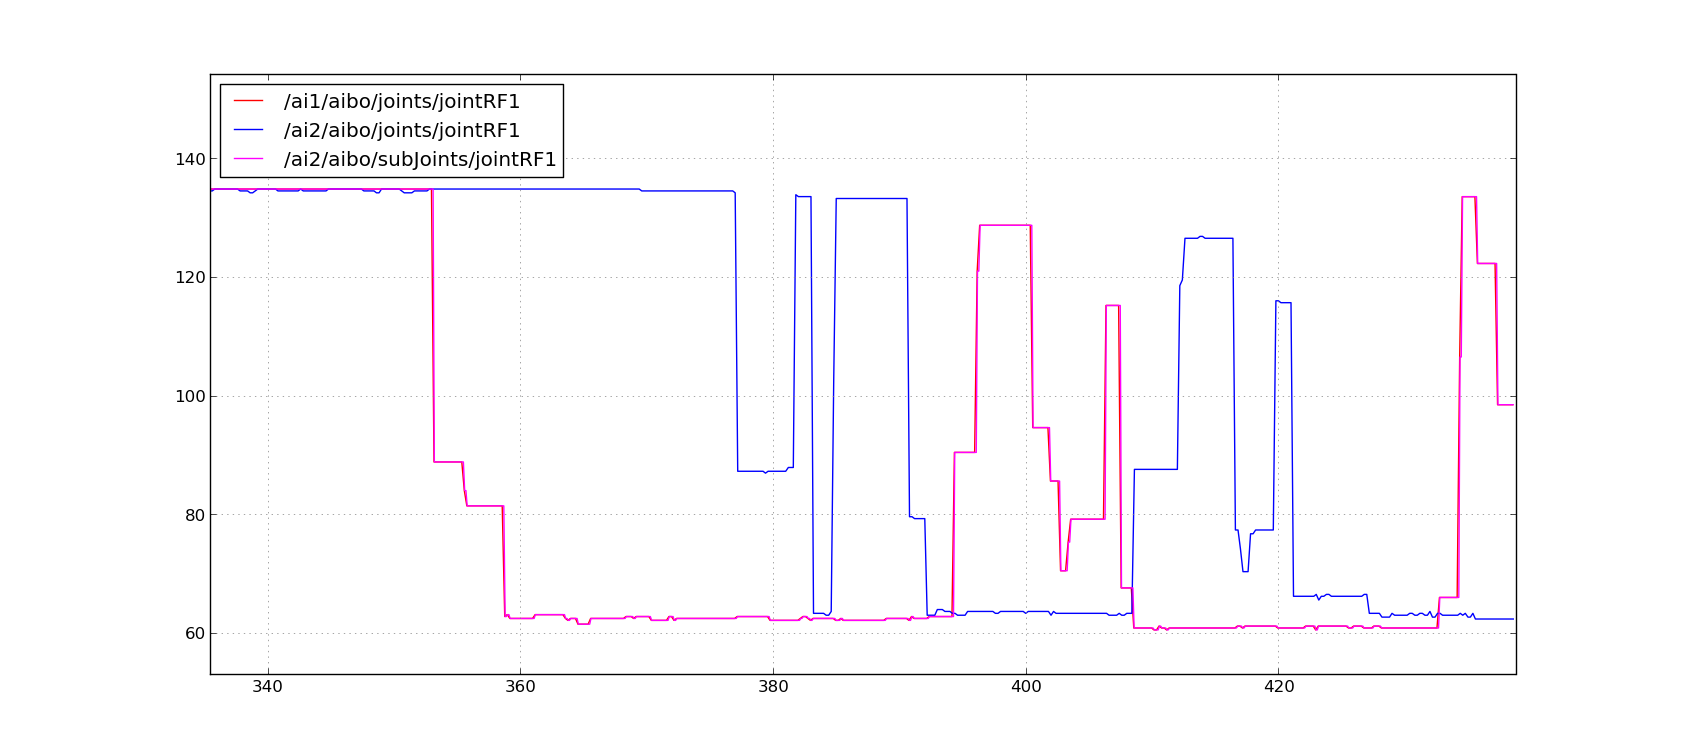
\includegraphics[scale=0.41]{images/mimic/malo5hz.png}
	 \caption{Posición de la articulación del AIBO movido manualmente, en rojo, la enviada al segundo AIBO, en fucsia y la del AIBO que hace la imitación, en azul.}
  \label{fig:resumimic2}
\end{figure}


Tras aplicar el cambio sobre el callback de ROS se ha evitado el problema del bloqueo pero como se ve en la Figura \ref{fig:resumimic2} los resultados dejan mucho que desear y están lejos de permitir aplicaciones de control remoto o sincronización. 

\subsection{Paquete Aibo{\_}description }
Este paquete pretende ser el vinculo entre el AIBO y una de las herramientas más usadas de ROS para robots móviles, rviz\footnote{http://wiki.ros.org/rviz}. Rviz es un visualizador 3D para aplicaciones de robótica que permite visualizar un modelo, el entorno sensado o un mapa virtual. 

El paquete consta de dos partes diferenciadas, la creación de el modelo de AIBO para que pueda ser representada la imagen 3D y la implementación de un nodo que haga responder el modelo en tiempo real a lo que sucede en el robot real.

\subsubsection{El modelo}
Para generar un modelo, se debe editar un xml con formato URDF\footnote{http://wiki.ros.org/urdf}(Unified Robots Description Format) donde se especifican las dimensiones del robot, las articulaciones y sus movimientos, la geometría de las extremidades y parámetros físicos como la masa o la inercia.
Para el modelo del AIBO se han creado 22 partes y 21 articulaciones se han descartado para el modelo la boca y las orejas. En la Figura \ref{fig:aibourdf} Se puede ver un esquema de las articulaciones, las partes y la disposición de los ejes que conforman el modelo implementado en el archivo URDF.

\newpage
\begin{figure}[H]
	\centering
    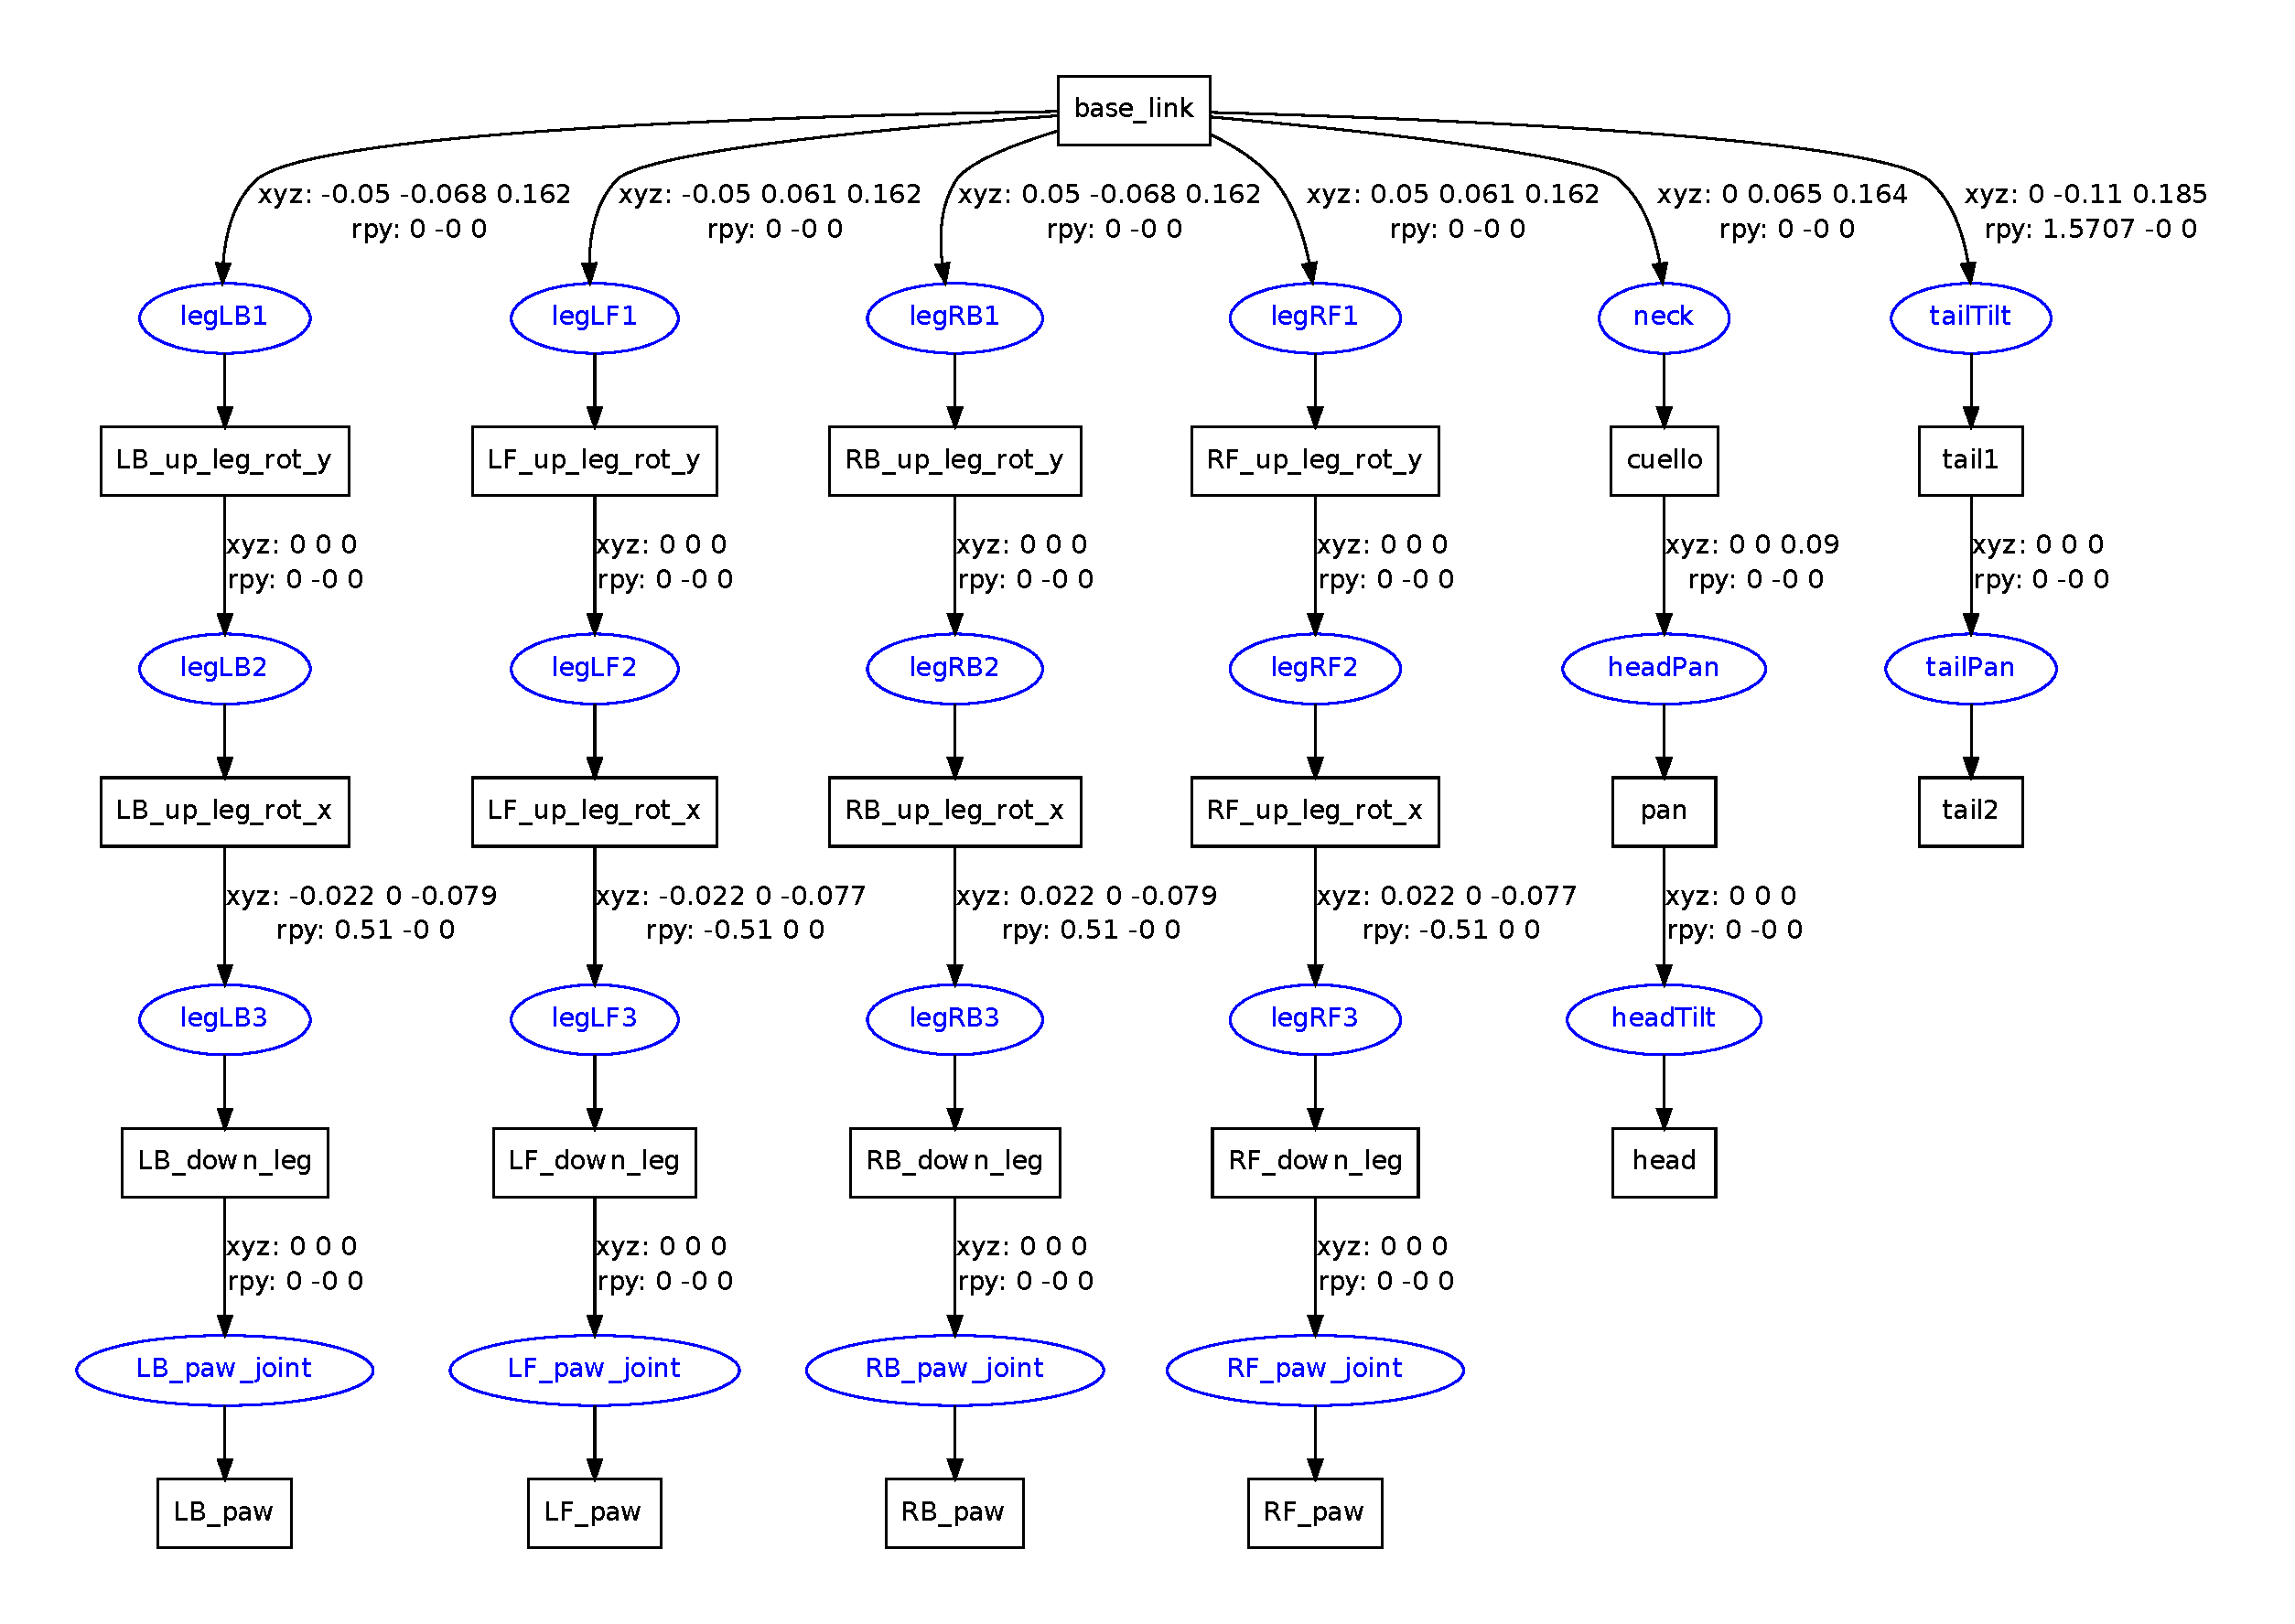
\includegraphics[scale=0.39]{images/Aibo.pdf}
	 \caption{Estructura del modelo URDF.}
  \label{fig:aibourdf}
\end{figure}

En  cada una de las partes se debe definir la geometría y sus dimensiones. Con el fin de darle un aspecto visual atractivo y mas semejante a al AIBO real la geometría ha sido  definida mediante archivos .stl que contienen las figuras de cada una de las partes. Los archivos stl se han obtenido de modificar un archivo stl que incluía un modelo solido de todo el AIBO. Se ha dividido, modificado las piezas usando las softwares de apoyo FreeCAD\footnote{http://freecadweb.org/} y Netfabb\footnote{http://www.netfabb.com/}. Finalmente el resultado es el mostrado en la Figura \ref{fig:aiborviz} donde se ve el modelo desde la ventana de rviz.
 
\begin{figure}[H]
	\centering
    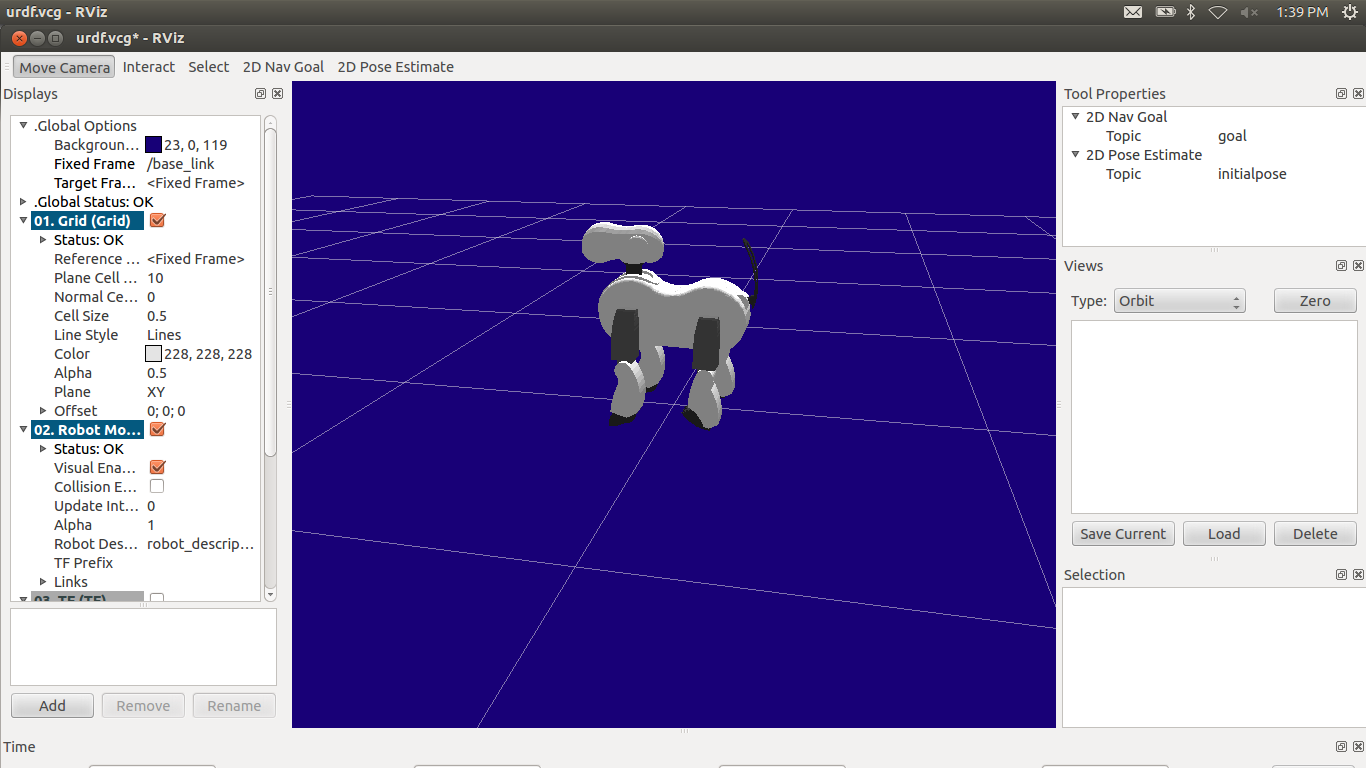
\includegraphics[scale=0.32]{images/aiborviz.png}
	 \caption{Modelo visto des de el framework de rviz.}
  \label{fig:aiborviz}
\end{figure}
\subsubsection{El nodo state{\_}publisher}\label{nodoSP}
El nodo state{\_}publisher esta creado por un programa escrito en C++ (state{\_}publisher.cpp) y su principal función es estar suscrito al tópico \texttt{/aibo{\_}server/ aibo/joints}, donde se están publicando las posiciones las articulaciones del robot real, y las publica en un tópico llamado \texttt{joint{\_}states} al que ya se podrá comunicar rviz. Además envía la transformada del modelo cinemático.
La estructura del programa es la siguiente:
\begin{itemize}
\item Inicialización:
\begin{itemize}
\item Inicialización del nodo state{\_}publisher.
\item Inicialización del \textit{publisher}.
\item Inicialización del \textit{subscriber}.
\item Inicialización del \textit{broadcaster}: Canal de envió de la transformada. 
\end{itemize}
\item Declaración de mensajes:
\begin{itemize}
\item joint{\_}state: a trabes del que se publica el estado de las articulaciones.
\item odom{\_}trans: a través del que se enviará la transformada.
\end{itemize}
\item Bucle de ROS:
\begin{itemize}
\item Actualización del estado de las articulaciones.
\item Actualización de la transformada.
\item Envío de las articulaciones.
\item Envío de la transformada.
\item Revisión del callback. 
\end{itemize}
\item Callback del \textit{subscriber}:
\begin{itemize}
\item Adquisición de los valores de las articulaciones.
\end{itemize}
\end{itemize}
\subsubsection{Estructura}
Para la realización del paquete se han implementado o modificado los siguientes archivos:
\begin{itemize}
\item Incluir en el manifest.xml los paquetes de ROS necesarios:
\begin{itemize}
\item roscpp: Permite usar el API de ROS para C++.
\item urdf: Permite leer y parsear archivos urdf.
\item std{\_}msg: Permite importar mensajes estándar.
\item tf: Permite la crear el modelo cinemático inverso.
\item aibo{\_}server: Permite importar los mensajes propios.  
\end{itemize}
\item Implementación del archivo state{\_}publisher.cpp, Sección \ref{nodoSP}.
\item Carpeta urdf: se incluye el archivo Aibo.urdf donde está descrito el modelo.
\item Carpeta meshes: se incluyen los archivo stl con los modelos 3D de las partes del modelo.
\item Carpeta launch: incluye el archivo aibomod.launch. En el se definen los nodos y los parámetros a partir de los que será posible la visualización del modelo con rviz.
\begin{itemize}
\item Se asigna al parametro robot{\_}description el archivo Aibo.urdf.
\item Se lanza un nodo del tipo robot{\_}state{\_}publisher del paquete con el mismo nombre. Dicho nodo esta suscrito al tópico joint{\_}states sobre el que publica el nodo implementado, state{\_}publisher, y se encarga de parsear el modelo que haya bajo el parámetro robot{\_}state{\_}publisher y publica sobre el tópico /tf el cual usa rviz para generar el movimiento del modelo.
\item Se lanza un nodo del tipo state{\_}publisher.
\item Se lanza un nodo del tipo rviz con la configuración deseada.
\end{itemize}
\end{itemize}

En la Figura \ref{fig:aibostack} se puede observar como queda la estructura de los nodos con el visualizador rviz y el nodo aibo{\_}server en funcionamiento.

\begin{figure}[H]
	\centering
    
\includegraphics[scale=0.26]{images/graphModel.pdf}
	 \caption{Estructuras de los nodos de ROS con aibo{\_}server y el modelo visualizado con rviz.}
  \label{fig:aibostack}
\end{figure}
\newpage

\section{Presupuesto}
El coste total del proyecto asciende a 18.200{\euro} de los cuales el 82,42{\%} es en concepto de personal. En ser un proyecto fundamentalmente de software y todo el software usado es con licencia libre, des de el sistema operativo hasta el procesador de textos, los costes asociados al material solo vienen dados por el coste de la plataforma de estudio.

\subsection{Coste material}
\begin{table}[H]
\begin{center}
\begin{tabulary}{\textwidth}{|C|C|C|C|}
\hline
\textbf{Concepto}&\textbf{Coste unitario [{\euro}/unid.]} & \textbf{Cantidad} & \textbf{Coste total [\euro]} \\ \hline
AIBO ERS-7 & 1600& 2& 3200 \\ \hline

\end{tabulary}
\end{center}
\caption{Coste material detallado.\label{costmat}}
\end{table}
\subsection{Coste personal}
\begin{table}[H]
\begin{center}
\begin{tabulary}{\textwidth}{|C|C|C|C|}
\hline
\textbf{Concepto}&\textbf{Coste horario [{\euro}/hora]} & \textbf{Horas} & \textbf{Coste total [\euro]} \\ \hline
Estudio preliminar & 30& 300& 9000 \\ \hline
Diseño y depuración & 30& 150& 4500 \\ \hline
Programación& 15& 100& 15000 \\ \hline
\textbf{Total}& & 550& 15000 \\ \hline
\end{tabulary}
\end{center}
\caption{Coste personal detallado.\label{costper}}
\end{table}

\newpage

\section{Impacto ambiental}
El objetivo de este proyecto conlleva como causa inmediata el incremento de la vida útil de una plataforma ya en desuso. Por tanto no se está perjudicando el medio ambiente en absoluto, sino que por lo contrario se está reciclando un objeto que en otro caso acabaría por desecharse en poco tiempo.

En cuanto al impacto ambiental asociado al uso de la plataforma que en cierta manera se ahorra se puede dividir en chasis, electrónica y batería.

El chasis esta hecho de ABS (Acrilonitrilo Butadieno Estireno, en inglés). Se trata de un termoplástico amorfo difícil de reciclar y en su proceso de fabricación usa acrilonitrilo, que es altamente tóxico.

Tanto la electrónica como las baterías contienen metales pesados altamente contaminantes si no son tratados correctamente.

Las baterías son de iones de litio y aunque su impacto ambiental de las cuales no esta muy claro, tienen potencial de contaminar el subministro de agua subterránea debido a que contiene metales como cobalto.


\newpage
\section*{Conclusiones}
\addcontentsline{toc}{section}{Conclusiones}


Cuando se trabaja con sistemas reales uno se da cuenta que no todo funciona de forma ideal y que un algoritmo que debería funcionar conlleva a múltiples errores o respuestas no esperadas. En éste caso concreto se ha visto como las comunicaciones que establecía el lenguaje base elegido no eran tan buenas como se esperaba. Los resultados dejan mucho que desear y no permiten ni aseguran el buen funcionamiento de posteriores aplicaciones basadas en el módulo implementado. De todas formas se ha alcanzado el objetivo siguiendo la metodología establecida en primer momento, se a implementado un modulo de ROS que permite integrar la plataforma AIBO, formado por los paquetes \textbf{aibo{\_}server} y \textbf{aibo{\_}description}. Estos paquetes se pueden encontrar en el repositorio (url del github) y están disponibles para su uso o modificación con tal de complementarlos o mejorar los resultados. Además se pretende colgar, fuera del alcance del proyecto, los paquetes y la documentación necesaria para su uso en la pagina de ROS con tal de contribuir y aportar un grano de arena al desarrollo de software libre.

Este proyecto deja un camino abierto a las posibles mejoras y complementos. Entre otros la integración del modulo de visión y audio usando URBI como se ha echo. Por otra parte dado que los resultados han demostrado no ser un modulo demasiado robusto cabria la posibilidad de implementar el mismo modulo partiendo OPEN-R, eliminando de esta manera una capa de programación intermedia, URBI, que posiblemente ralentice y empeore la comunicación entre cliente y servidor. En cuanto al modelo y el nodo que permite su integración con rviz podría completarse añadiendo los sensores del AIBO como los acelerómetros, los infrarrojos, los sensores de presión y contacto y la camera, permitiendo proyectos de odometría.

A nivel personal y educativo este proyecto ha servido para poner a prueba la capacidad de análisis y de resolución de problemas. Ha ayudado a tener un amplio conocimiento de de uno de los frameworks relacionados con la robótica mas usados del momento. Además a ayudado a mejorar las habilidades de desarrollo de software con los lenguajes C++ y python. 

\newpage
\section*{Agradecimientos}
\addcontentsline{toc}{section}{Agradecimientos}
Este proyecto no podría haber sido posible sin el apoyo de la familia y amigos que han sido fuente de motivación y ánimo.

Un especial agradecimiento a los tutores de éste proyecto, Manel Velasco y Cecilio Angulo tanto por su implicación y atención como por facilitar el material y el espacio de trabajo.

Por último agradecer al doctor Ricardo Tellez de quien salió la idea de este proyecto y quien le dio su primer impulso, además de su apoyo y consejo durante su realización.
\newpage
\clearpage
\addcontentsline{toc}{section}{Referencias}
\begin{thebibliography}{99}
\bibitem{aibo}
	Arevalillo-Herráez, Miguel and Moreno-Picot, Salvador and Millán, Vicente Cavero,
	\emph{Arquitectura para Utilizar Robots AIBO en la Enseñanza de la Inteligencia Artificial.}
	2012.
	\url{http://dblp.uni-trier.de/db/journals/ieee-rita/ieee-rita6.html#Arevalillo-HerraezMM11},
	
\bibitem{ros}
	Quigley, Morgan and Conley, Ken and Gerkey, Brian P. and Faust, Josh and Foote, Tully and Leibs, Jeremy and Wheeler, Rob and Ng, Andrew Y.,
	\emph{ROS: an open-source Robot Operating System}.
	2009.
\bibitem{libroblanco}
	CEA, Comité Español de Automàtica,
	\emph{El libro blanco de la robótica en España}.
	2011.
	
\bibitem{OPEN-R PG}
  Sony Corporation,
  \emph{OPEN-R Programmer's Guide}.
  2004.

\bibitem{urbiref}
	Baillie,
	\emph{URBI: Towards a Universal Robotic Low-Level Programming Language}.
	2005.
	
\bibitem{xavi}
	Xavier Perez,
	\emph{Vision-based Navigation and Reinforcement Learning Path Finding for Social Robots}.
	2010.
\bibitem{metod}
	Ángel Montero Mora, Gustavo Méndez Muñoz, José Ramon Dominguez Rodriguez,
	\emph{Metodologías de diseño de comportamientos para AIBO ERS7}.
	2009.
\bibitem{robocup}
	RoboCup, \url{http://www.robocup2014.org/}
\bibitem{morales}
	Jesus Morales,
	\emph{Localización de objetos y posicionamiento en el escenario de RoboCup Four-Legged con un robot AIBO}.
	2007.  
\bibitem{jesus}
	Jesús Martinez Gómez, 
	\emph{Diseño de un teleoperador con detección de colisiones para robots AIBO}. 			2006.
\bibitem{riki}
	Ricardo A. Tellez,
	\emph{Aibo Programming}.
	\url{http://www.ouroboros.org/aibo.html}
\bibitem{TekkQuickRef}
	Ethan Tira-Thompson,
	\emph{Tekkotsu Quick Reference}, ERS-7, Tekkotsu 3.0.
\bibitem{tekkTut}
	David S. Touretzky and Ethan J. Tira-Thompson, 
	\emph{Exploring Tekkotsu Programming on Mobile Robots}.
	Carnegie Mellon University,
	2010.
	\url{http://www.cs.cmu.edu/~dst/Tekkotsu/Tutorial/contents.shtml}
\bibitem{urbi}
	\emph{URBI},
	\url{http://www.urbiforge.org/index.php/Main/Robots}
	
\bibitem{urbicmd}
	Jean-Christophe Baillie,
	\emph{URBI Doc for Aibo ERS2xx ERS7 Devices documentation}.
	2005.

\bibitem{euslisp}
	ROS new by kwc,
	\emph{EusLisp now open source}.
	2010.
	\url{http://www.ros.org/news/2010/07/euslisp-now-open-source.html}
\bibitem{kecsap}
	Kecsap,
	\emph{Porting URBI 2.x for AIBO}.
	2010.
	\url{http://kecsapblog.blogspot.com.es/2010/12/porting-urbi-2x-for-aibo.html}
	
	
\end{thebibliography}

\label{Referencies}
%\addcontentsline{toc}{section}{Referències}
%\bibliography{Aibobib.bib}

\appendix
\clearpage % o \cleardoublepage
\addappheadtotoc
\appendixpage

\section{Manual de usuario}
\subsection{Requisitos previos}
Es necesario antes de instalar los paquetes seguir los siguientes pasos.
\begin{itemize}
\item Instalar Ubuntu 12.04 (Precise) de 32 bits.

\item Descargar librería liburbi 1.5 para C++:

\url{http://www.gostai.com/downloads/urbi/1.5/}
\begin{itemize}
\item Descomprimir la librería, que ya está compilada, en el directorio \texttt{/usr} del sistema.
\end{itemize}
\item Instalar de ROS. 

\begin{itemize}
\item Preparar el ordenador apara aceptar el software de ROS:


\begin{lstlisting}[language=bash]
  sudo sh -c 'echo "deb http://packages.ros.org/ros/ubuntu precise main" > /etc/apt/sources.list.d/ros-latest.list'
\end{lstlisting}

\item Preparación las claves:
\begin{lstlisting}[language=bash]
	wget http://packages.ros.org/ros.key -O - | sudo apt-key add -
\end{lstlisting}

\item Instalación:
\begin{lstlisting}[language=bash]
	sudo apt-get install ros-fuerte-desktop-full
\end{lstlisting}

\item Preparación del entorno:
\begin{lstlisting}[language=bash]
	echo "source /opt/ros/fuerte/setup.bash" >> ~/.bashrc
. ~/.bashrc
\end{lstlisting}

\item Crear un workspace:
\begin{lstlisting}[language=bash]
	rosws init ~/fuerte_workspace /opt/ros/fuerte
\end{lstlisting}
\begin{lstlisting}[language=bash]
	sudo apt-get install python-rosinstall
\end{lstlisting}
\item Crear un sandbox donde irán los nuevos paquetes y añadir al ROS{\_}PACKAGE{\_}PATH:
\begin{lstlisting}[language=bash]
	mkdir ~/fuerte_workspace/sandbox
	rosws set ~/fuerte_workspace/sandbox
	echo "source ~/fuerte_workspace/setup.bash" >> ~/.bashrc
. ~/.bashrc
	
\end{lstlisting}
\item Confirmación de la correcta instalación del entorno:

Al ejecutar:
\begin{lstlisting}[language=bash]
	echo $ROS_PACKAGE_PATH
\end{lstlisting}
Se debe obtener algo similar a:
\begin{lstlisting}[language=bash]
	/home/your_user_name/fuerte_workspace/sandbox:/opt/ros/fuerte/share:/opt/ros/fuerte/stacks
\end{lstlisting}
\end{itemize}

\item Asegurarse que los siguientes paquetes de ROS han sido instalados:
\begin{itemize}
\item rviz:
\begin{lstlisting}[language=bash]
	rospack find rviz
\end{lstlisting}
\item urdf
\begin{lstlisting}[language=bash]
	rospack find urdf
\end{lstlisting}
\item robot{\_}state{\_}publisher
\begin{lstlisting}[language=bash]
	rospack find robot_state_publisher
\end{lstlisting}
\item tf
\begin{lstlisting}[language=bash]
	rospack find tf
\end{lstlisting}


Deben devolver la ubicación del paquete.
\end{itemize}

\item Descargar los paquetes:
\begin{itemize}
\item aibo{\_}server:

\url{https://github.com/Diamg/AiboRosPackages/tree/master/aibo_server}
\item aibo{\_}description

\url{https://github.com/Diamg/AiboRosPackages/tree/master/aibo_description}
\end{itemize}
\item Copiar la tarjeta de memoria, Figura \ref{fig:aiboMS} para el AIBO con URBI:

\url{https://github.com/Diamg/AiboRosPackages/tree/master/MS_URBI}
\begin{figure}[H]
	\centering
    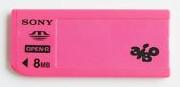
\includegraphics[scale=0.5]{images/MS.jpg}
	 \caption{Tarjeta de memoria para AIBO.}
  \label{fig:aiboMS}
\end{figure}

\item Configuración de la conexión wireless con el AIBO.

Editar el archivo WLANDFLT.txt que se encuentra en el directorio /OPEN-R/SYSTEM/CONF de la tarjeta de memoria del AIBO.

El archivo contiene los siguientes variables:
\begin{itemize}
\item HOSTNAME: Especifica el nombre de AIBO que se está usando.
\item ETHER{\_}IP: La IP que usará el AIBO.
\item ETHER{\_}NETMASK: La mascara de subred.
\item IP{\_}GATEWAY: La IP a traves de la que el AIBO accederá a la red.
\item ESSID: Nombre de la red inalámbrica.
\item WEPENABLE: con valor 1 si existe contraseña en la red o 0 en caso contrario.
\item WEPKEY: contraseña de la red.
\item APMODE: Método de conexión del AIBO.
\begin{itemize}
\item 0 para conexión punto a punto.
\item 1 para conexión con ruter.
\item 2 para conexión automática en el método que primero se lo permita.
\end{itemize}
\item CHANEL: especificar el canal para el modo punto a punto.
\end{itemize}
La configuración por defecto es:

HOSTNAME = AIBO

ETHER{\_}IP = 10.0.1.100

ETHER{\_}NETMASK = 255.255.255.0

IP{\_}GATEWAY = 10.0.1.1

ESSID = AIBONET

WEPENABLE = 1

WEPKEY = AIBO2

APMODE = 2

CHANNEL = 3 
\end{itemize}

\subsection{Instalación}
\begin{itemize}
\item Guardar los paquetes en el workspace de ROS.
\item Ejecutar en un terminal:
\begin{lstlisting}[language=bash]
	rosmake --pre-clean aibo_server
	rosmake --pre-clean aibo_description
\end{lstlisting}


\end{itemize}
\subsection{aibo{\_}server}
Ejecutar en terminal:
\begin{lstlisting}[language=bash]
	rosrun aibo_server aibo_server arg[1] arg[2]
\end{lstlisting}



Donde:
\begin{itemize}
\item arg[1] es la IP del AIBO.
\item arg[2] es la frecuencia en numero entero a la que se desea que vaya el bucle de ROS (La frecuencia por defecto y recomendada son 5 Hz).
\end{itemize}


\subsubsection{Tópicos}

El nodo aibo{\_}server permite subscribirse a los siguientes tópicos:
\begin{itemize}
\item \texttt{/aibo{\_}server/aibo/infrared}:
 
Da la información de los tres infrarojos del AIBO guardada en forma de mensaje de tipo aibo{\_}server/IRArrays.  

\item \texttt{/aibo{\_}server/aibo/touch}:

D la información de los sensores de presión de la barbilla, la cabeza y los tres de la espalda en un mensaje de tipo aibo{\_}server/TouchArray.

\item \texttt{/aibo{\_}server/aibo/accel}:

Da la información de los acelerometros en un mensaje de tipo aibo{\_}server/Accel.

\item \texttt{/aibo{\_}server/aibo/joints}:

Da la información de las posiciones de las articulaciones en un mensaje de tipo aibo{\_}server/Joints.

\item \texttt{/aibo{\_}server/aibo/paws}:

Da la información de los sensores de contacto de las tres patas en forma de mensaje del tipo aibo{\_}server/BumperArray.


\end{itemize}
Y publicar sobre el tópico:
\begin{itemize}
\item \texttt{/aibo{\_}server/aibo/subJoints}:

Permite controlar la posición de las articulaciones en un mensaje de tipo aibo{\_}server/Joints.

\end{itemize}

\subsubsection{Mensajes}
\begin{itemize}
\item aibo{\_}server/IRArrays

\begin{lstlisting}[language=bash]
	Header header
	sensor_msgs/Range[] IRs
\end{lstlisting}

El array de mensajes de tipo std{\_}msgs/Range esta ordenado:
\begin{itemize}
\item sensor del pecho.
\item sensor del distancias cortas.
\item sensor de distancias largas.
\end{itemize}

\item sensor{\_}msgs/Range

\item aibo{\_}server/TouchArray

\begin{lstlisting}[language=bash]
	Header header
	float64[] touch
\end{lstlisting}


Los sensores están ordenados en la array de la siguiente forma:

\begin{itemize}
\item sensor de la barbilla
\item sensor de la espalda delantero
\item sensor de la espalda del medio.
\item sensor de la espalda trasero.
\item sensor de la cabeza.
\end{itemize} 

\item aibo{\_}server/Accel:

\begin{lstlisting}[language=bash]
	Header header
	float64 x
	float64 y
	float64 z
\end{lstlisting}
\begin{itemize}
\item x: Valor del acelerometro en el eje x.
\item y: Valor del acelerometro en el eje y.
\item z: Valor del acelerometro en el eje z.
\end{itemize}

\item aibo{\_}server/Joints
\begin{lstlisting}[language=bash]
	Header header
	float64 jointLF1
	float64 jointLF2     
	float64 jointLF3     
	float64 jointLH1     
	float64 jointLH2 
	float64 jointLH3 
	float64 jointRF1
	float64 jointRF2
	float64 jointRF3
	float64 jointRH1
	float64 jointRH2
	float64 jointRH3
	float64 tailPan
	float64 tailTilt
	float64 headTilt
	float64 headPan
	float64 headNeck
	float64 mouth

\end{lstlisting}

Donde:
\begin{itemize}
\item jointLF1: Articulación de rotación del hombro del de la pata izquierda delantera.
\item jointLF2: Articulación de apertura del hombro de la pata izquierda delantera.
\item jointLF3: Articulación del codo de la pata izquierda delantera.  
\item jointLH1: Articulación de rotación del hombro del de la pata izquierda trasera.     
\item jointLH2: Articulación de apertura del hombro de la pata izquierda trasera.
\item jointLH3: Articulación del codo de la pata izquierda delantera.
\item jointRF1: Articulación de rotación del hombro del de la pata derecha delantera.
\item jointRF2: Articulación de apertura del hombro de la pata derecha delantera.
\item jointRF3: Articulación del codo de la pata derecha delantera.
\item jointRH1: Articulación de rotación del hombro del de la pata derecha trasera.
\item jointRH2: Articulación de apertura del hombro de la pata derecha trasera.
\item jointRH3: Articulación del codo de la pata derecha trasera.
\item tailPan: Articulación de la cola para el movimiento lateral.
\item tailTilt: Articulación de la cola para el movimiento vertical.
\item headTilt: Articulación de la cabeza para el movimiento vertical.
\item headPan: Articulación de la cabeza para el movimiento lateral.
\item headNeck: Articulación del cuello.
\item mouth: articulación de la boca.

\end{itemize}
\item aibo{\_}server/BumperArray
\begin{lstlisting}[language=bash]
	Header header
	float64[] paws
\end{lstlisting}

La array de paws esta ordenada con el siguiente orden:
\begin{itemize}
\item Delantero izquierdo.
\item Trasero izquierdo.
\item Delantero derecho.
\item Trasero derecho.
\end{itemize}
\end{itemize}

\subsection{aibo{\_}description}
Ejecutar en la terminal:
\begin{lstlisting}[language=bash]
	roslaunch aibo_description aibomod.launch
\end{lstlisting}


Con tal de vincular el modelo con un AIBO se debe lanzar también un nodo aibo{\_}server.

\newpage

\section{Scripts y programas}
\subsection{Adquisición del valor de una articulación con liburbi.}
\label{getDataOneLegC++}
\lstinputlisting[language=c++]{src/getDataOneLeg/getDataC++/getData.cpp}

\subsection{Adquisición del valor de una articulación con Python.}
\label{getDataOneLegPy}
\lstinputlisting[language=Python]{src/getDataOneLeg/getDataPython/getData.py}

\subsection{Envió de trayectoria punto a punto con liburbi.}\label{sinC}
\lstinputlisting[language=c++]{src/sinLegRead/sinLegC++/2Client/sinLeg.cpp}

\subsection{Envió de trayectoria punto a punto con Python.}\label{sinP}
\lstinputlisting[language=Python]{src//sinLegRead/sinLegPython/sinlegLF1.py}

\subsection{Envió de trayectoria punto a punto con ROS.}\label{sinlegROS}
\lstinputlisting[language=c++]{src/ROStests/sinlegROS.cpp}

\subsection{Modulo de imitación entre AIBOs.}\label{mimiccode}
\lstinputlisting[language=c++]{src/ROStests/mimic.cpp}

\end{document}
